%%%%%%%%%%%%%%%%%%%%%%%%%%%%%%%%%%%%%%%%%%%%%%%%%%%%%%%%%%%%%%%%%%%%%%%%
%                                                                      %
%     File: Thesis_Conclusions.tex                                     %
%     Tex Master: Thesis.tex                                           %
%                                                                      %
%     Author: Andre C. Marta                                           %
%     Last modified :  2 Jul 2015                                      %
%                                                                      %
%%%%%%%%%%%%%%%%%%%%%%%%%%%%%%%%%%%%%%%%%%%%%%%%%%%%%%%%%%%%%%%%%%%%%%%%

\chapter{Analysis}
\label{chapter:analysis}

\section{Overview of the $hh\rightarrow b\overline{b}b\overline{b}$ channel}
%- Signal cross section and final state signature \\
%- Pros and challenges of using the 4b final state \\
%- Main backgrounds (the ones we consider) and respective cross sections (leave for appendix discussion on other backgrounds, namely Higgs processes)\\

\begin{figure}
	\centering
	\begin{minipage}{.45\textwidth}
		\centering
		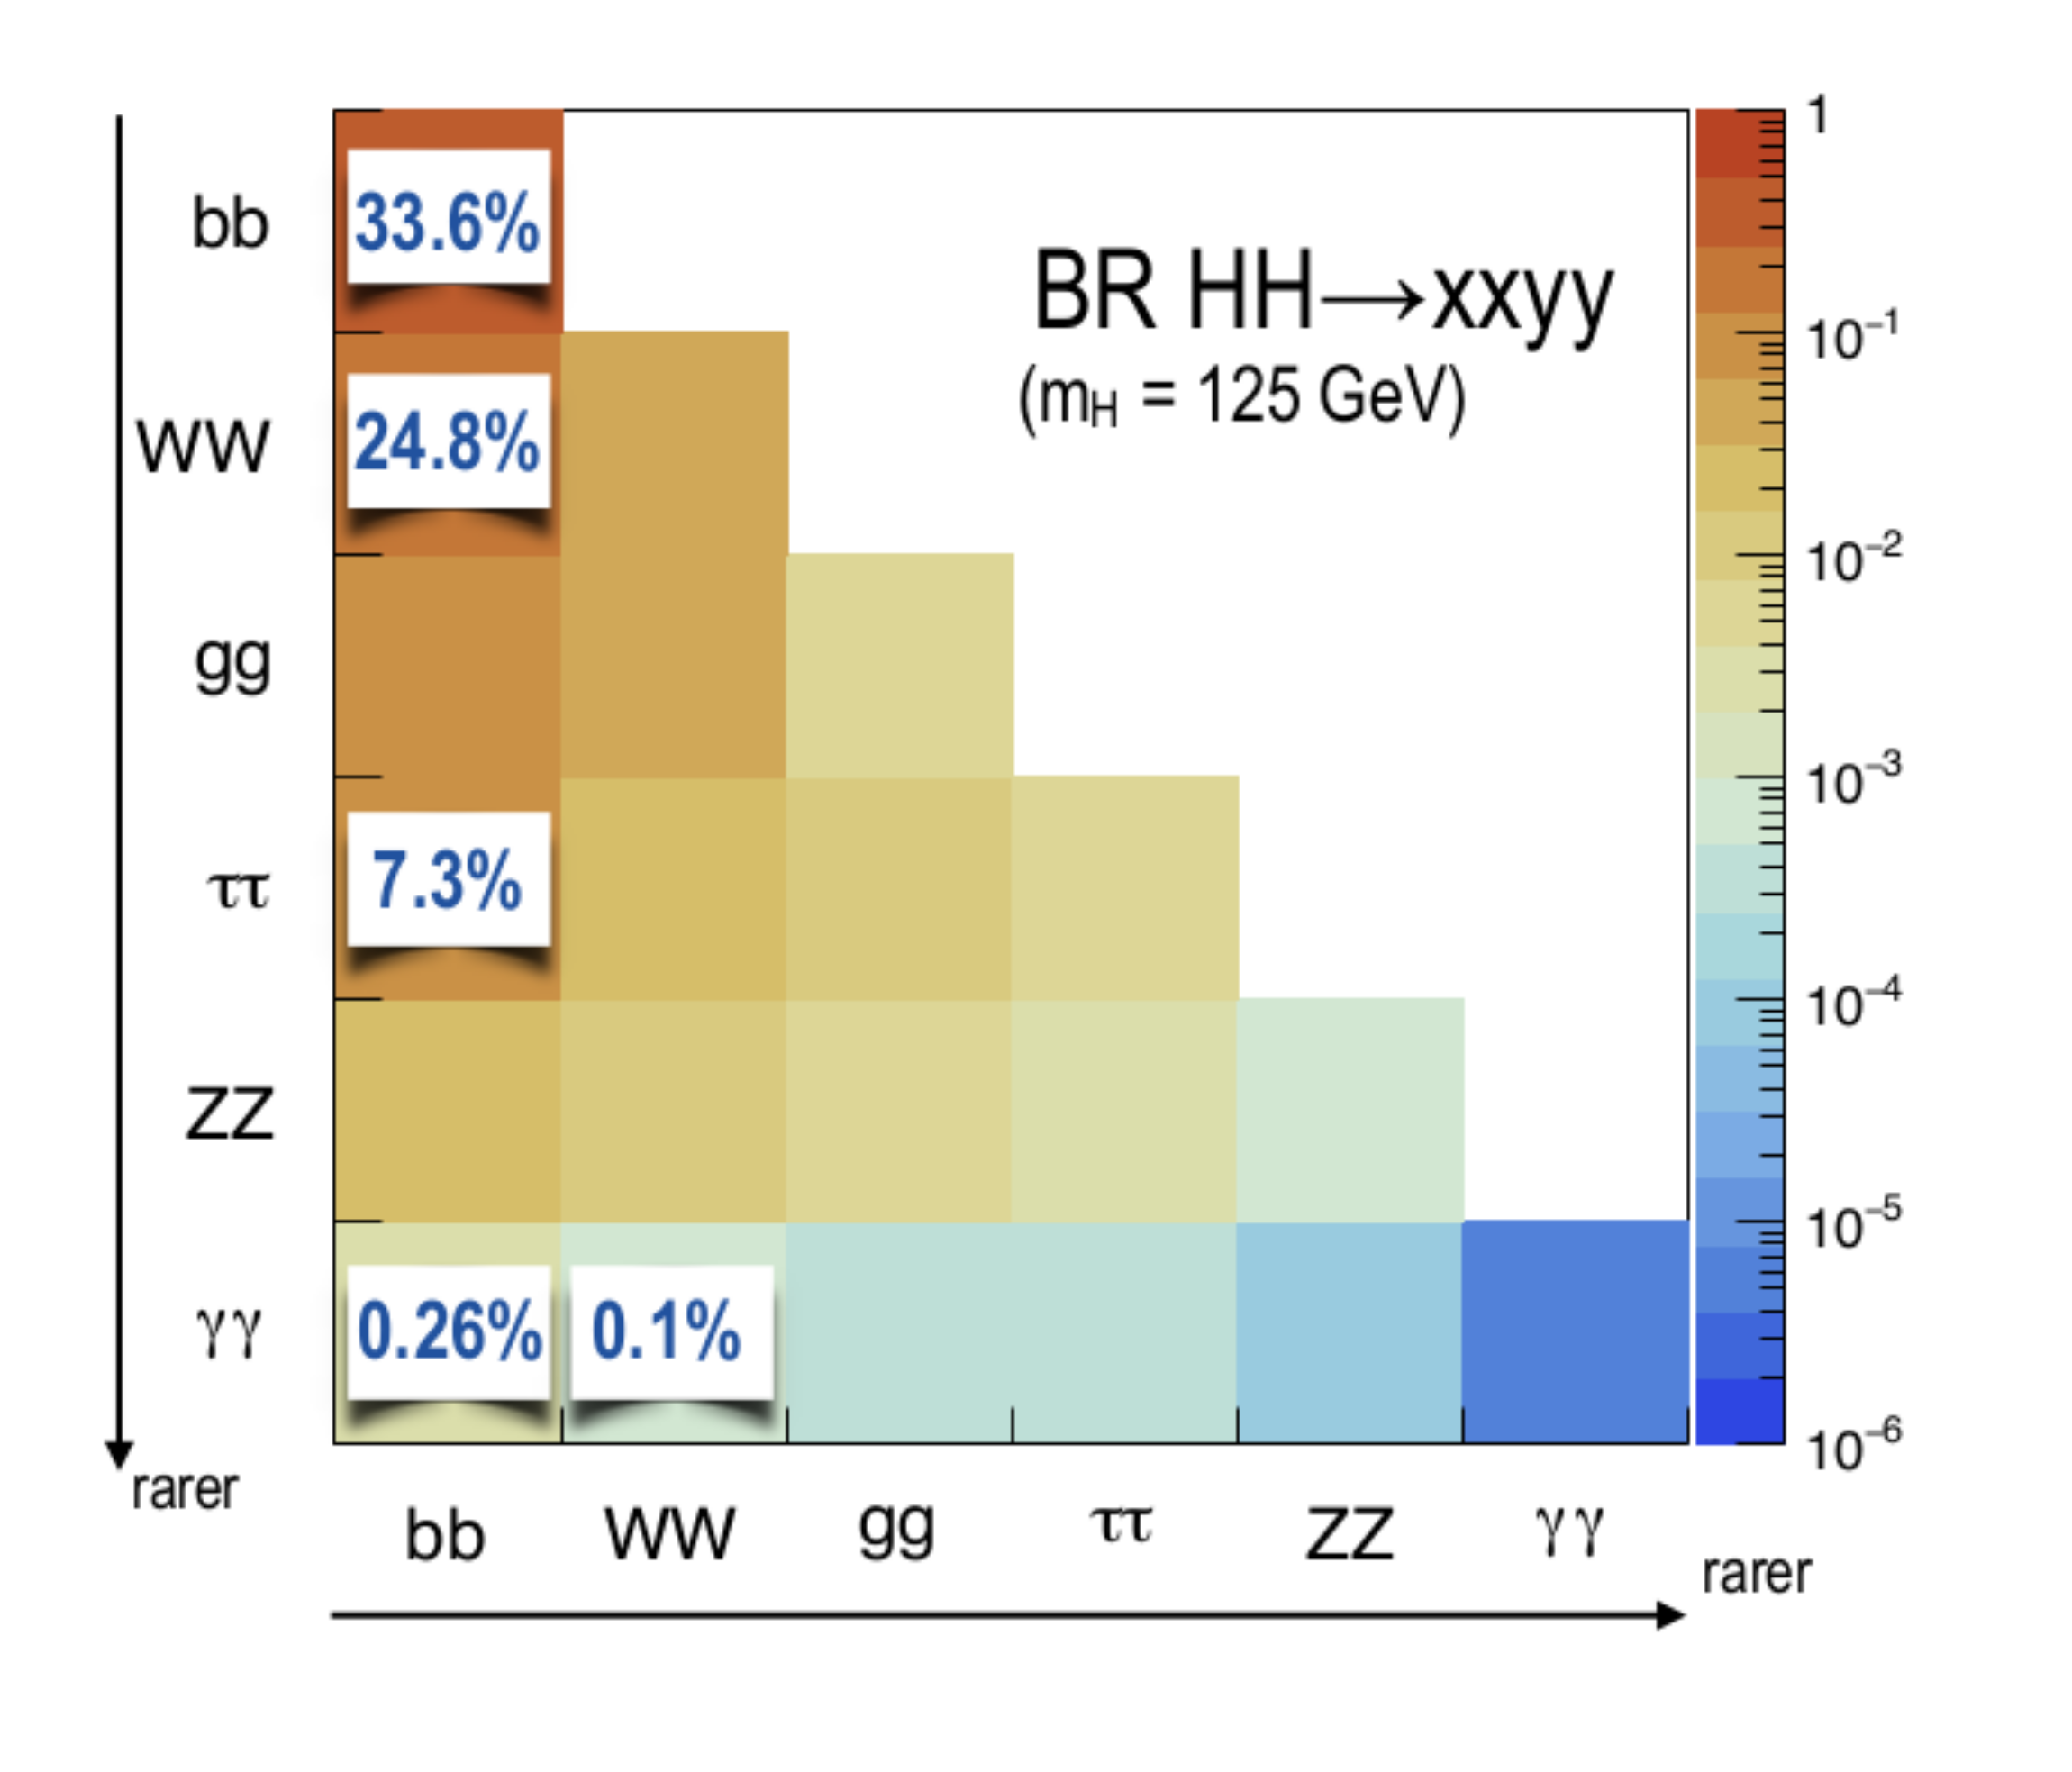
\includegraphics[width=\linewidth]{./Figures/hhBR.png}
	\end{minipage}%
	\begin{minipage}{.55\textwidth}
		\centering
		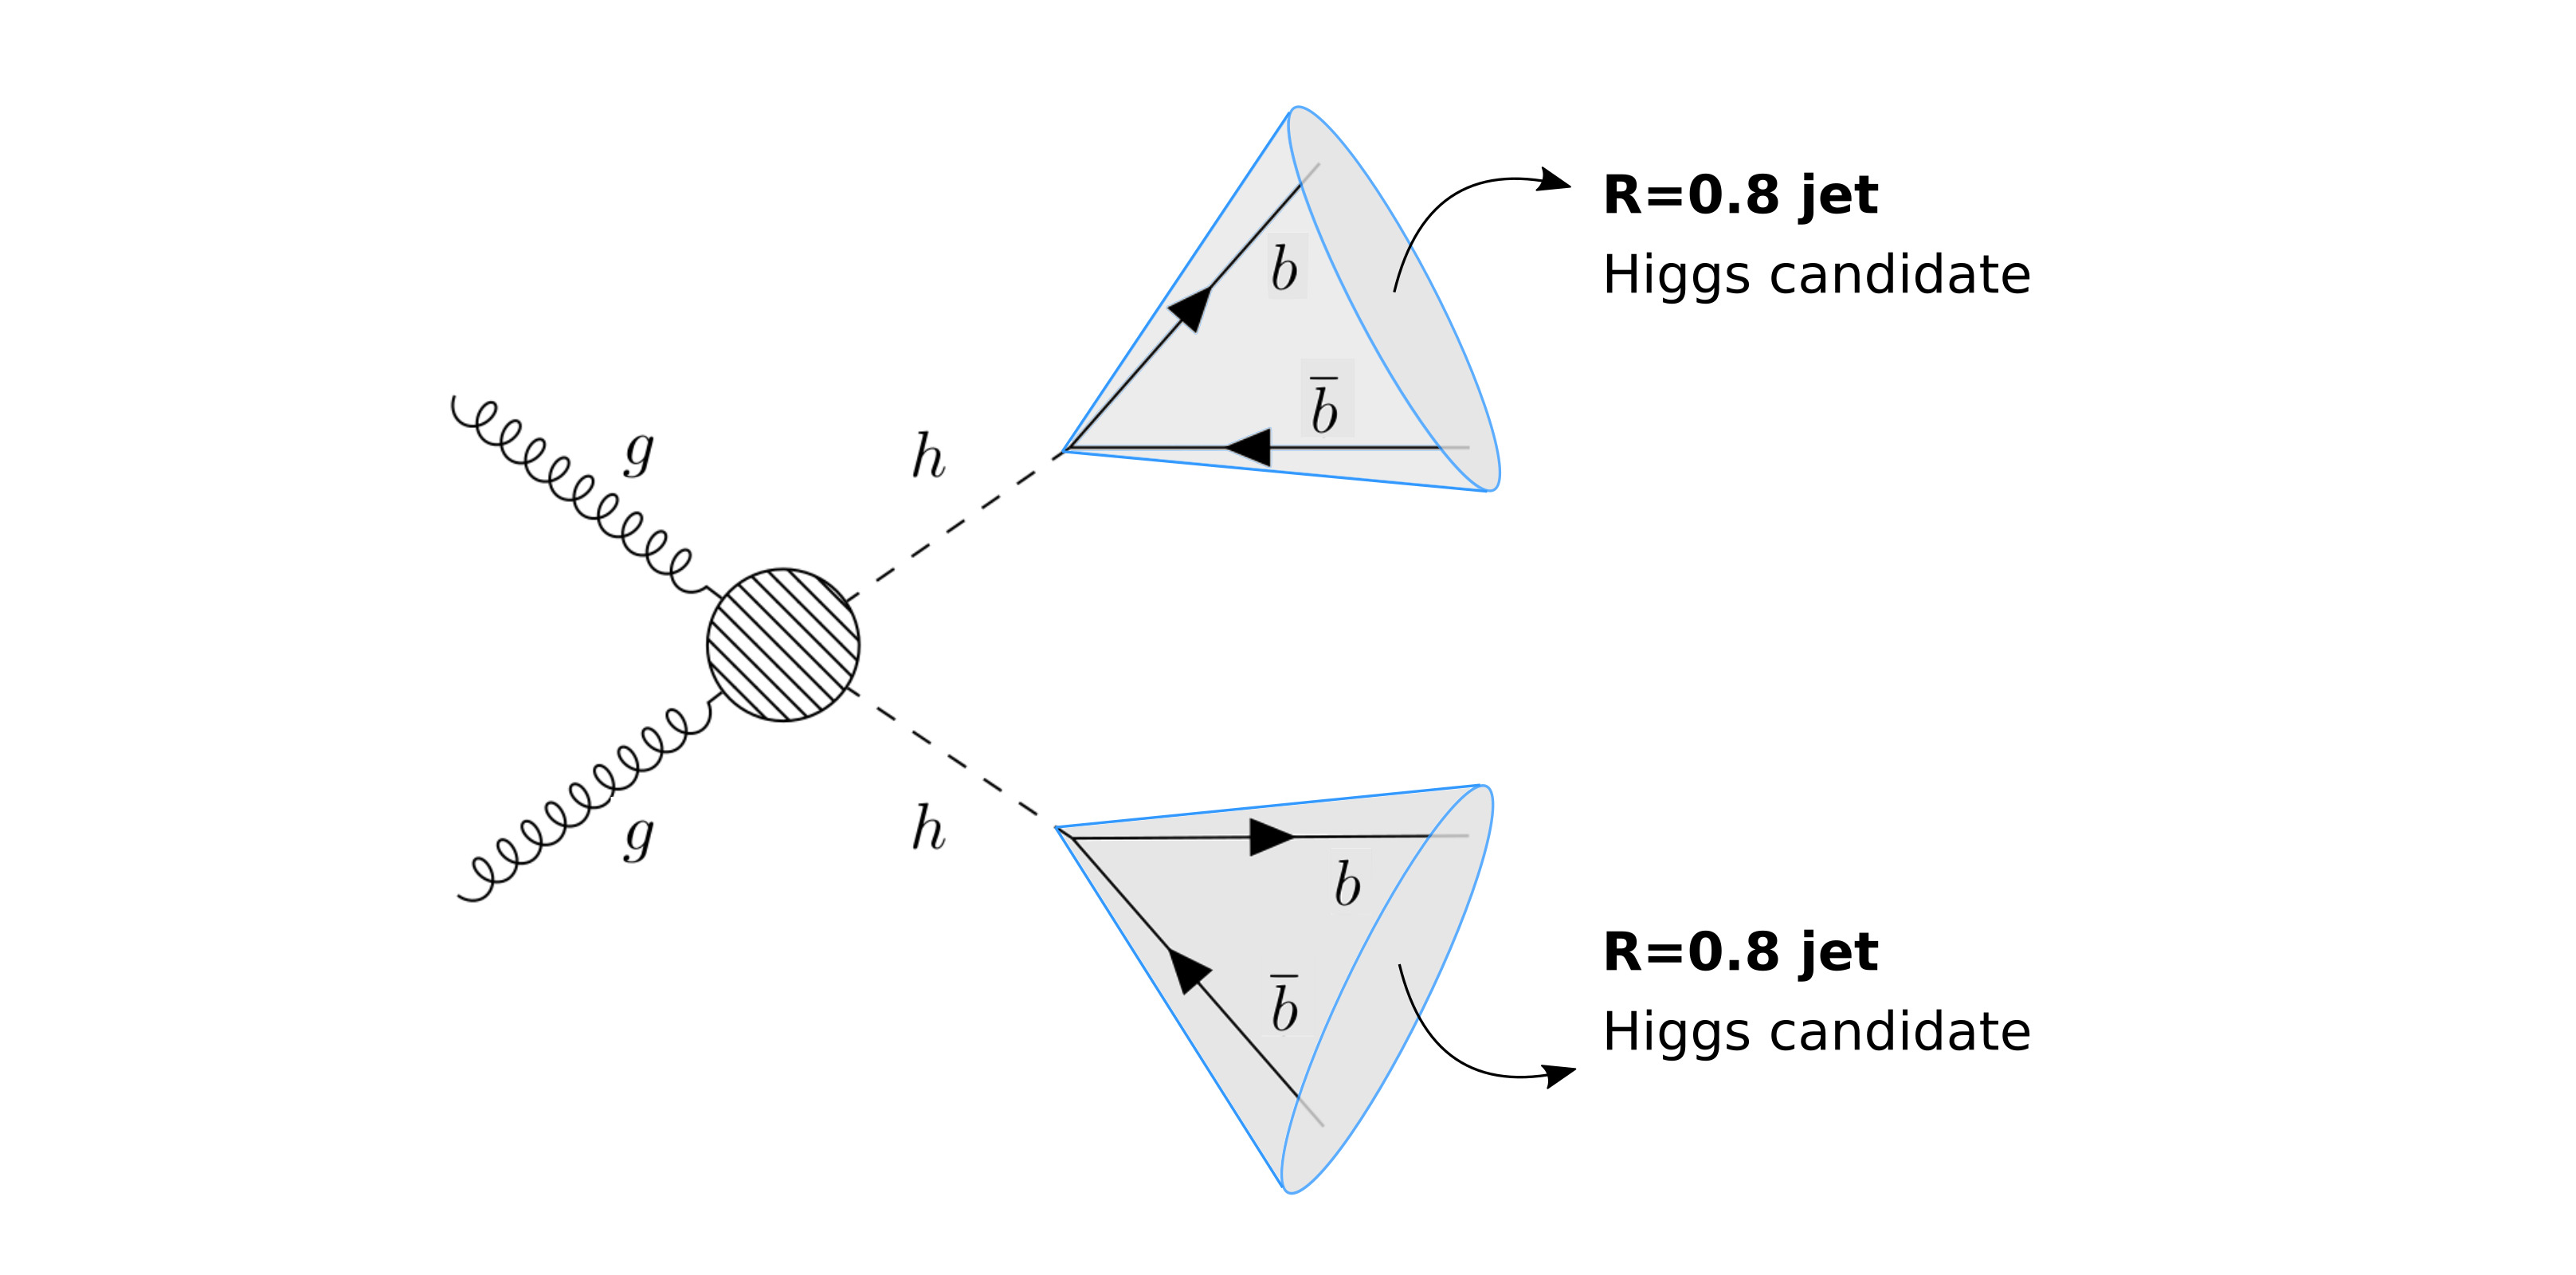
\includegraphics[trim={4cm 0 5cm 0},clip,width=\linewidth]{./Figures/boosted1.png}
	\end{minipage}
	\begin{minipage}[t]{0.45\textwidth}
		\caption*{(a)}
		%\label{fig1}
	\end{minipage}%%%
	\hfill
	\begin{minipage}[t]{0.55\textwidth}
		\caption*{(b)}
		%\label{fig2}
	\end{minipage}
	\caption{(a) Higgs pairs branching ratios, (b) event topology targeted by a boosted analysis.}
	\label{fig:boosted}
\end{figure}

%\begin{figure}
%	\centering
%	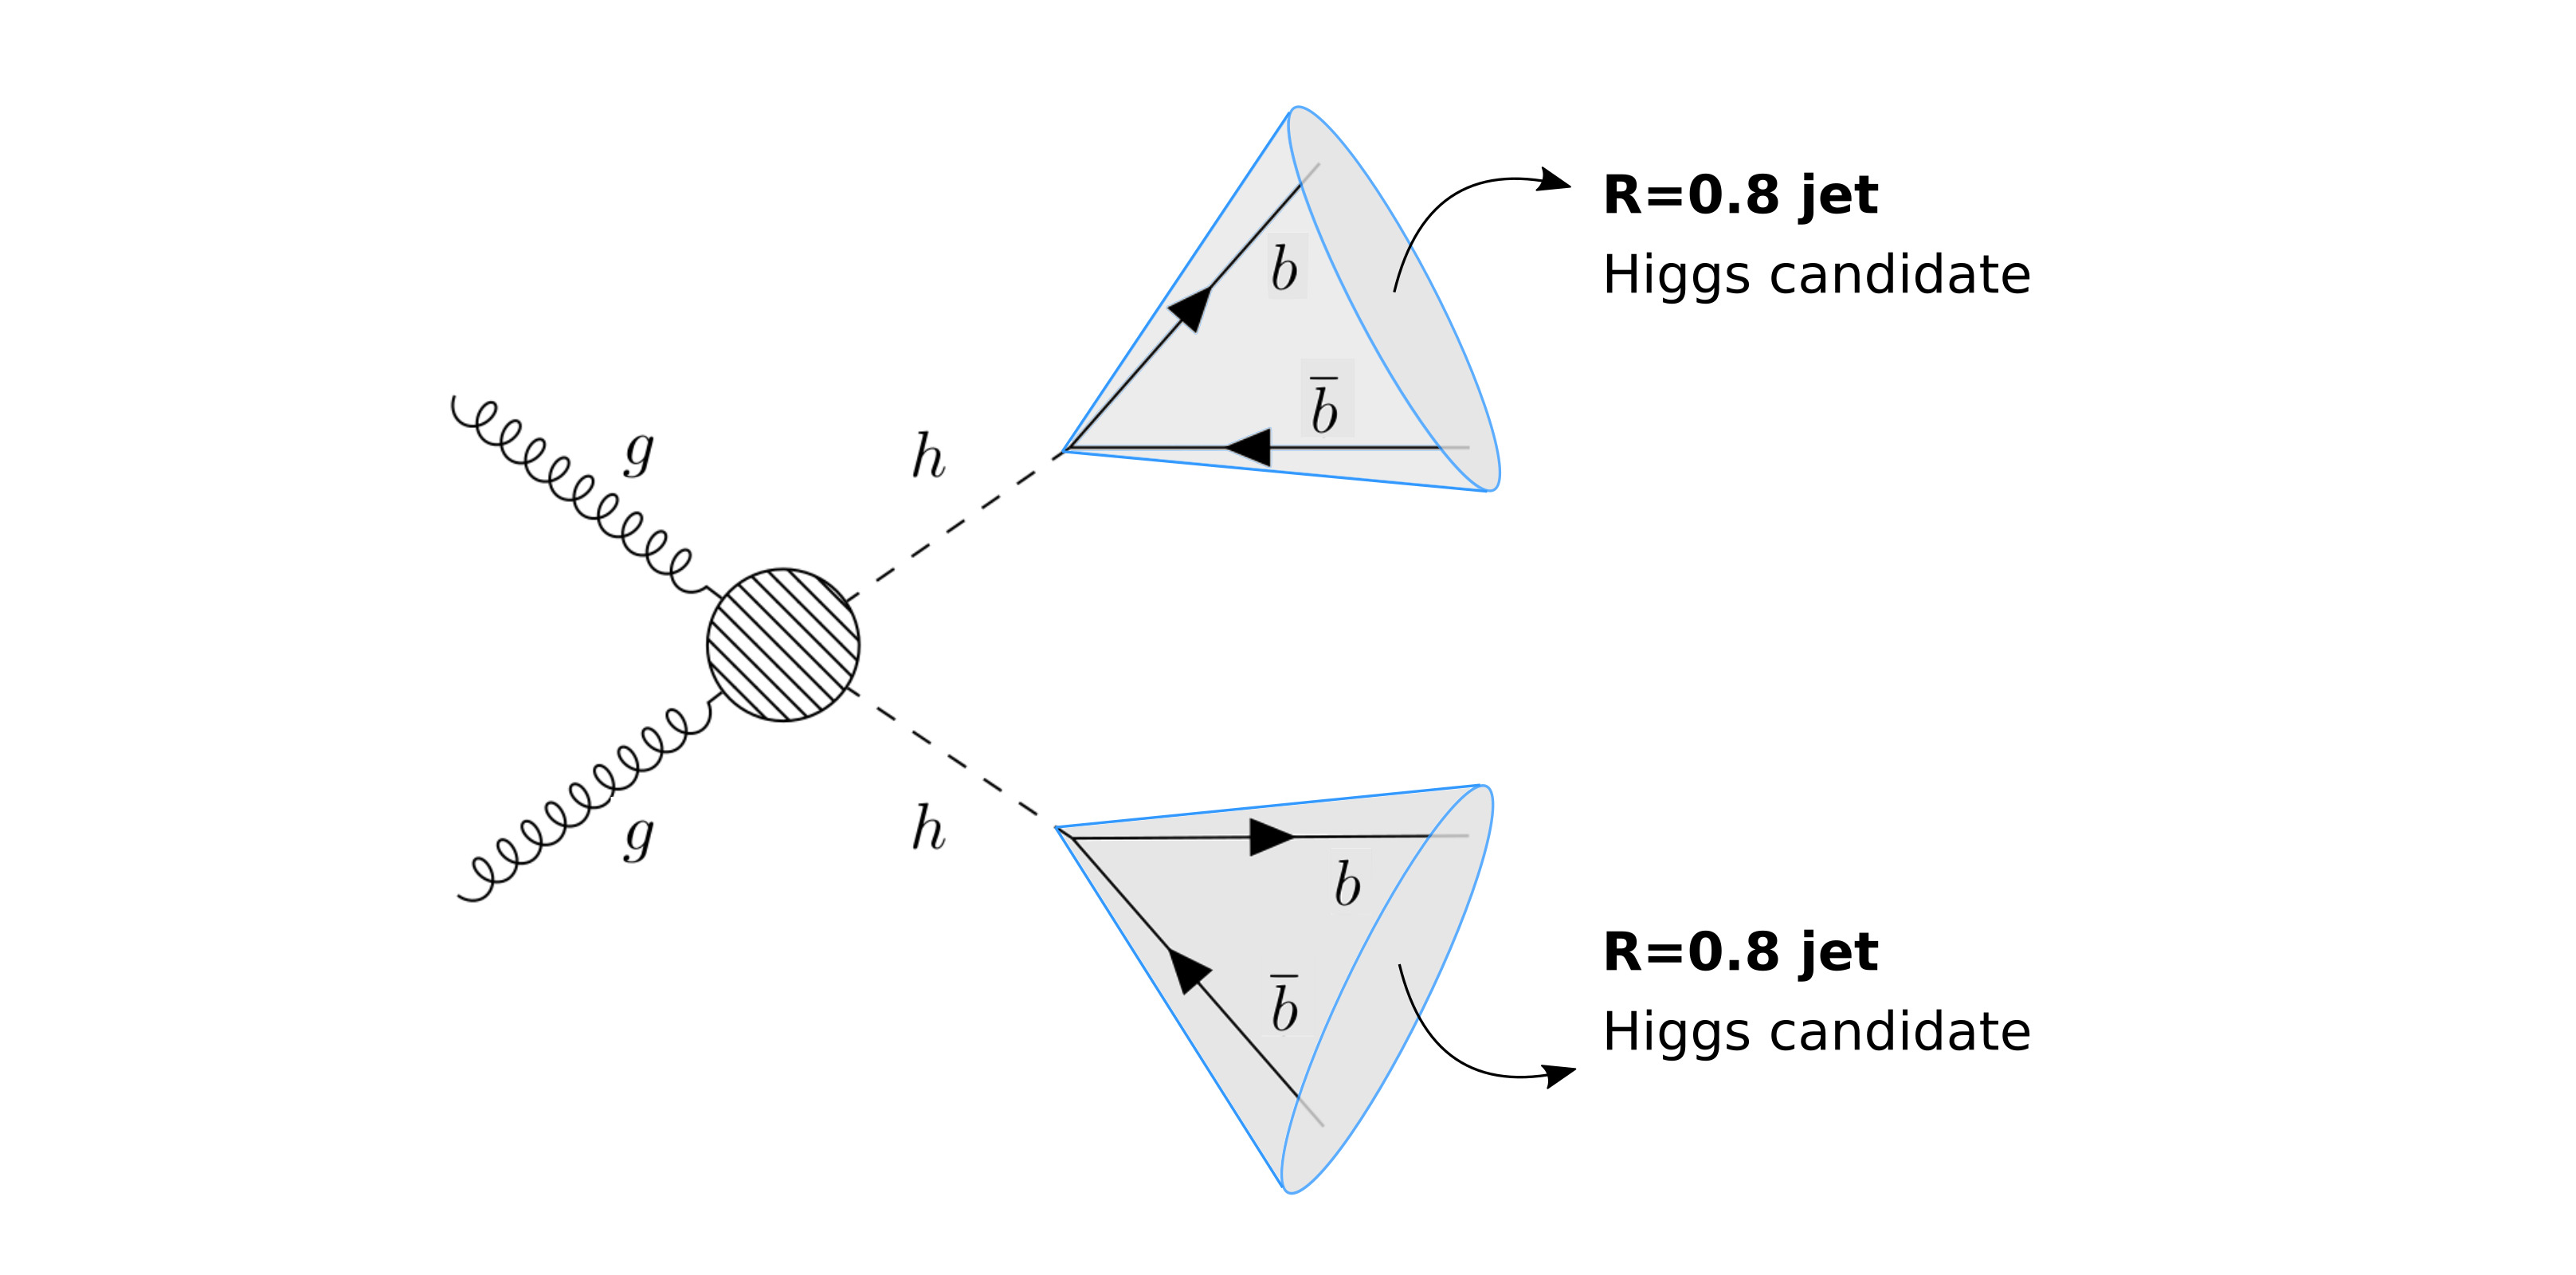
\includegraphics[width=\textwidth]{./Figures/boosted1.png}
%	%\hfill
%	%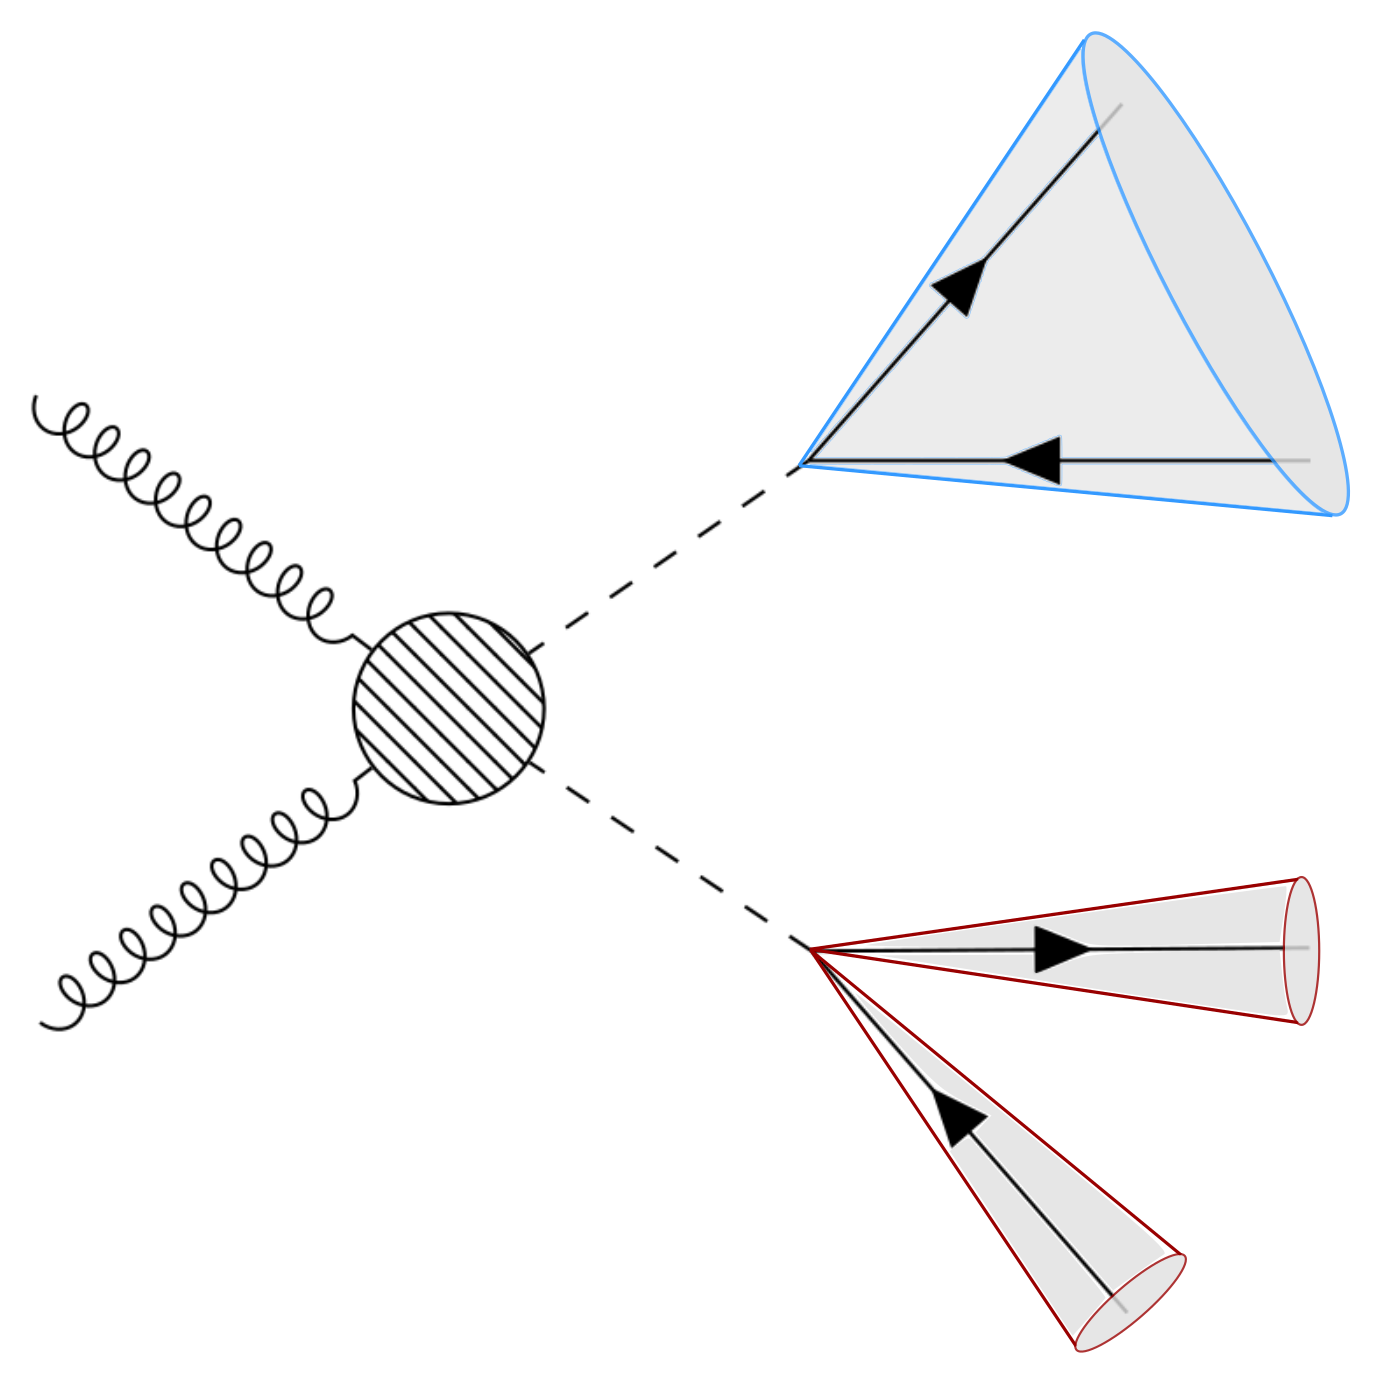
\includegraphics[width=.45\textwidth]{./Figures/inter.png}
%	\caption{Event topology targeted by the boosted analysis region. The blob represents the interaction between the gluons and the Higg bosons that is represented by the Feynman diagrams shown in figure \ref{fig:higgs_pair}.}
%	\label{fig:final_state}
%\end{figure}
%
%\begin{figure}
%	\centering
%	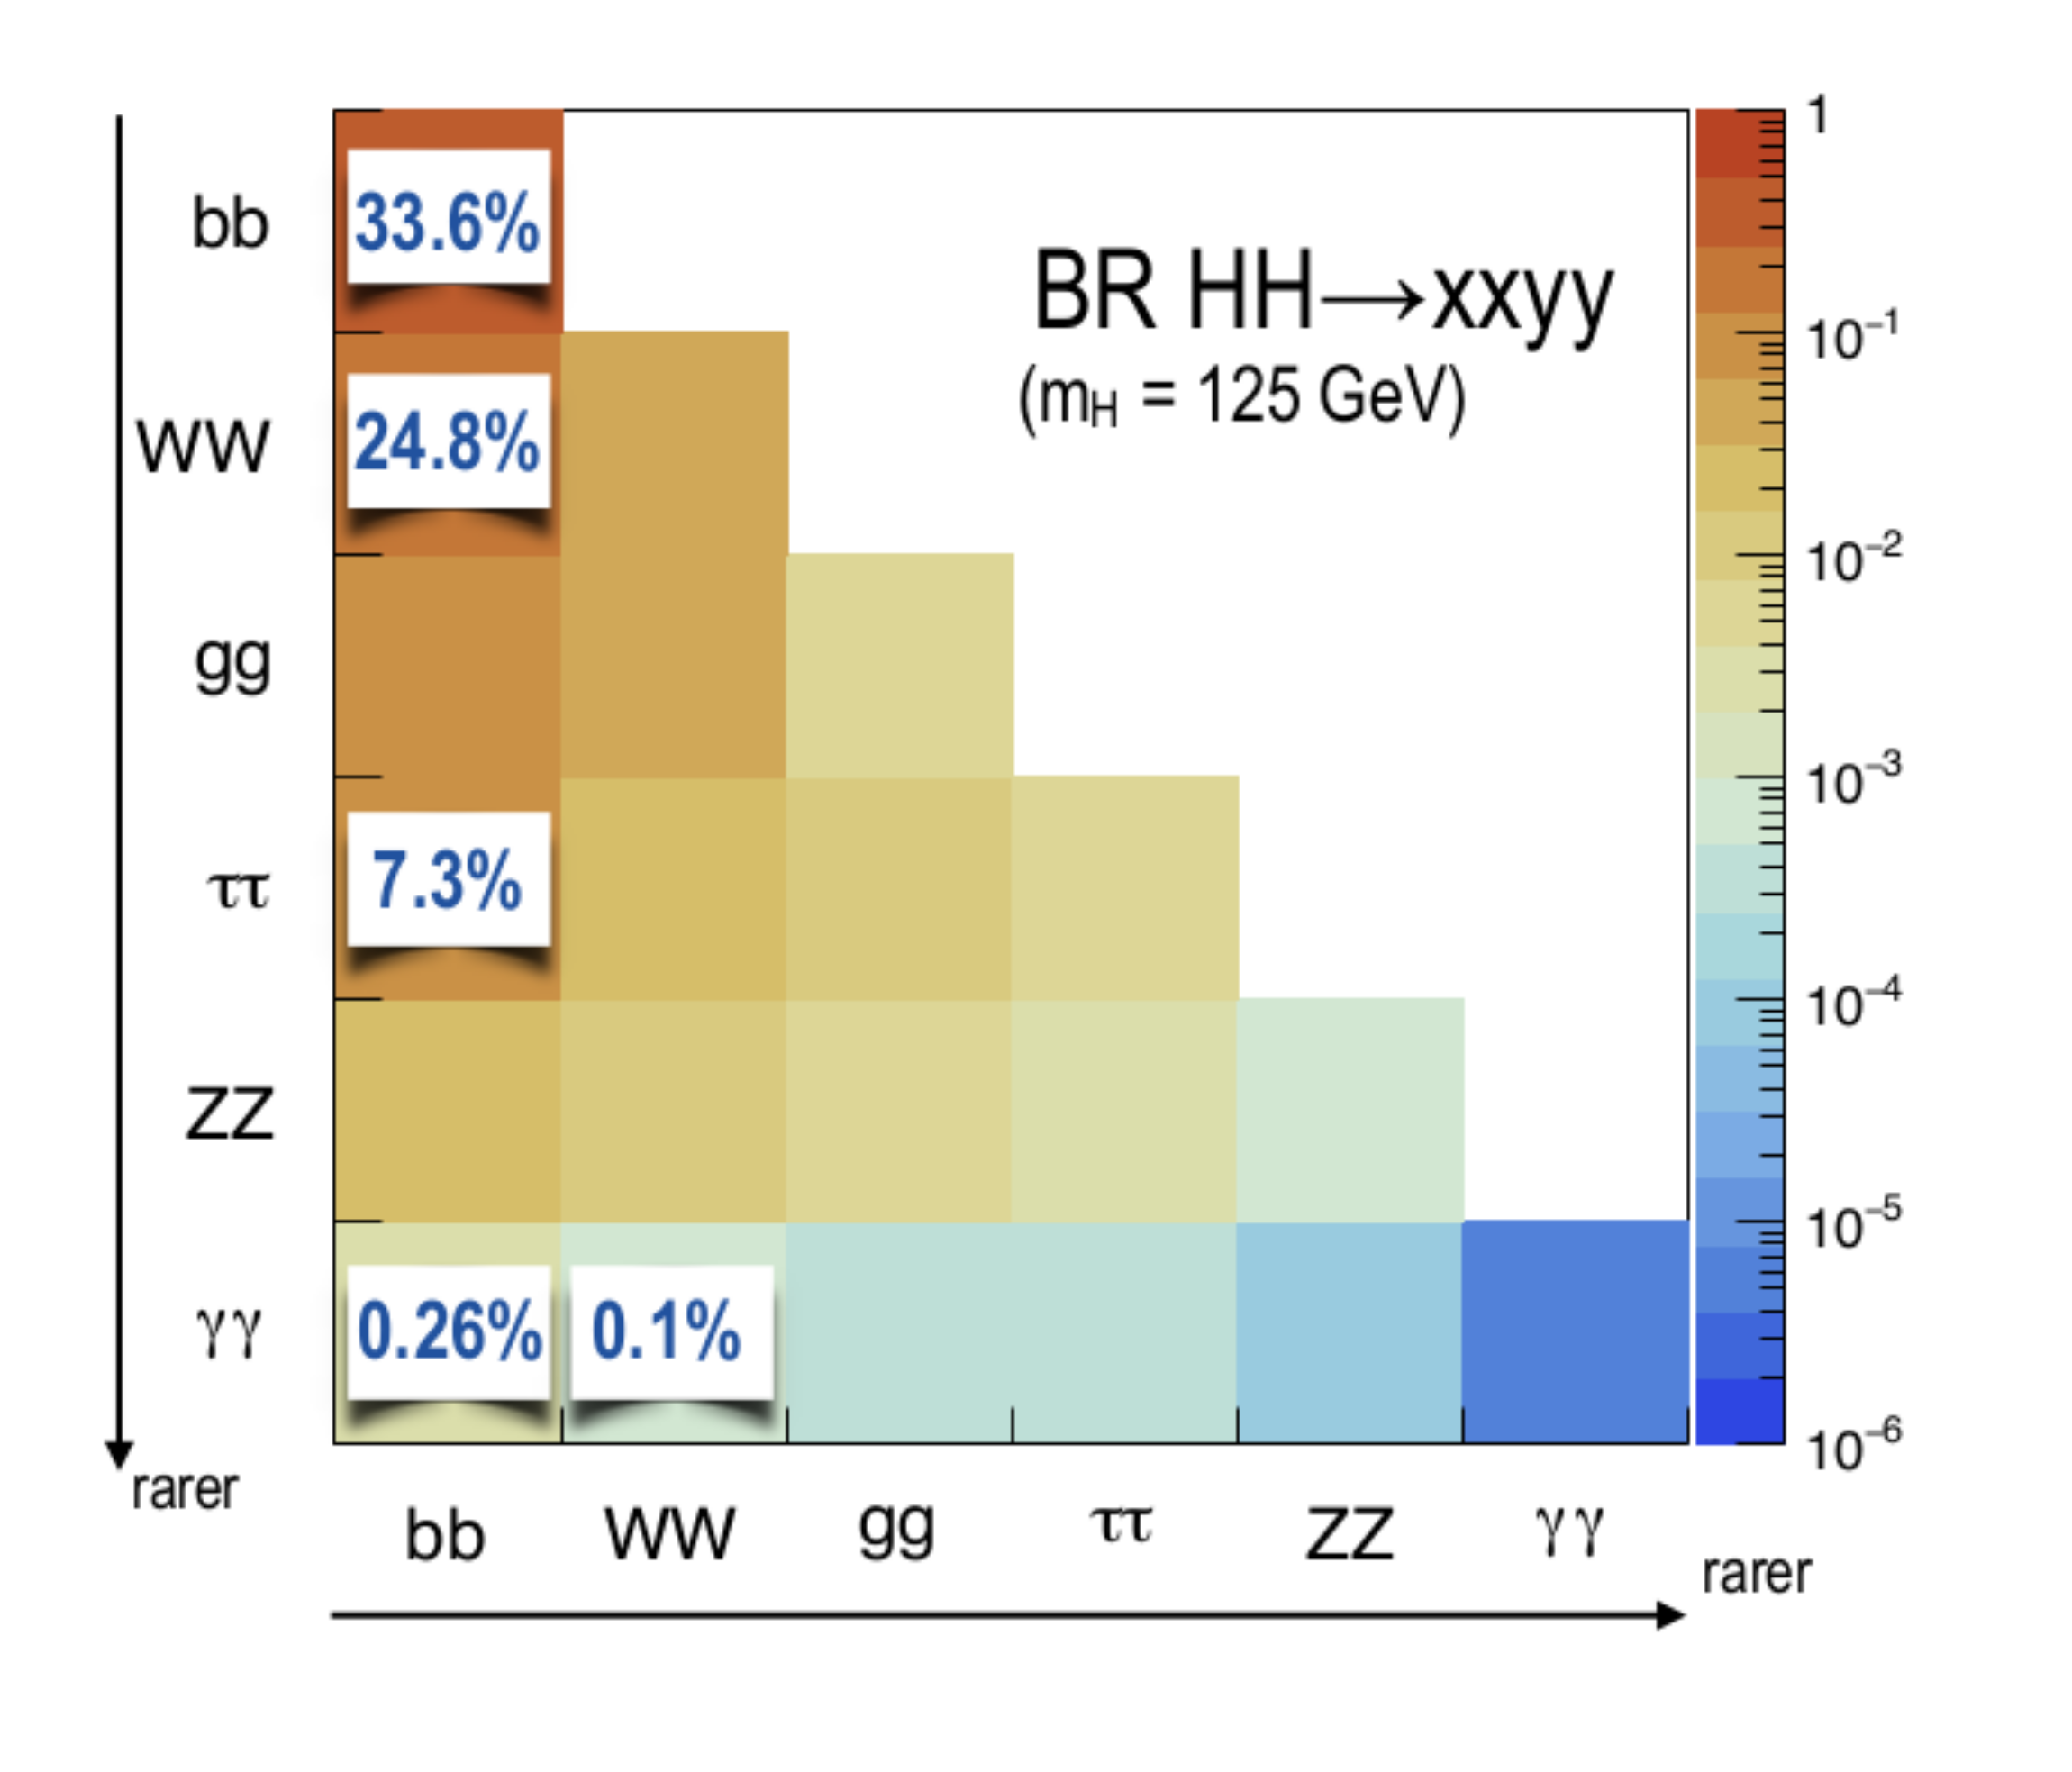
\includegraphics[width=0.6\textwidth]{./Figures/hhBR.png}
%	\label{fig:hhBR}
%	\caption{Higgs pair branching ratios.}
%\end{figure}

%The searches for Higgs pair production in the four b quarks final state benefit from the large BR of $h\rightarrow b\overline{b}$. 

For the SM Higgs, with a mass around $125$ GeV, the branching ratio of the $hh\rightarrow b\overline{b}b\overline{b}$ decay is approximately $33.6\%$, making it the most probable decay for Higgs pairs, as is illustrated in figure \ref{fig:boosted}(a).
%This leads to a cross section times BR of $\sim 0.7$ pb. 
However, in this channel, the main background is QCD multijet production that has a cross section several orders of magnitude larger than di-Higgs production in the SM, as table \ref{table:samples_summary} shows. Nonetheless, the jet $p_T$ distributions in this background have a very large yield close to zero and then fall very steeply while the signal has a much larger tail to high values of $p_T$ (see figure \ref{fig:h1h2_pt}(a)). This indicates that searches targeting the boosted kinematic regime may be the key to measure $hh\rightarrow b\overline{b}b\overline{b}$ using inclusive production.

In this work we target the boosted regime. In this kinematic region, the final state of the signal is characterized by two jets with a large radius parameter, each containing the two b quarks originated from the decay of one of the Higgs bosons, as figure \ref{fig:boosted}(b) illustrates. Extra jets are also expected to be reconstructed as a consequence of QCD radiation. 

The analysis presented here is performed using the Monte-Carlo samples described in chapter \ref{chapter:tools}. All samples including Higgs bosons assume $m_h=125$ GeV. The event selection criteria are designed to optimize the significance, given by $S/\sqrt{B}$, where $S$ and $B$ represent the number of signal and background events, respectively. 

%In addition, the jets produced by QCD interaction are more likely to be initiated by a gluon or a light quark. Therefore, tight b-tagging criteria and algorithms based on substructure variables can also help reject this background. 

\subsection{Event pre-selection}

%TO INCLUDE: \\
%- discussion on trigger requirements: important in real analysis\\
%- show and discuss some distributions: invariant mass (h, hh), momentum, tau21, delta eta (hh), more substructure variables (may be all that we considered relevant)\\
%- compare with other articles/analysis ? \\

We start by applying very simple and loose cuts that target events consistent with the boosted topology. Jets are reconstructed with the anti-$k_T$ algorithm with a radius parameter $R=0.8$. They are reconstructed from particle flow objects or calorimeter towers only. Both approaches were explored in this analysis.

We require at least two b-tagged $R=0.8$ jets. A $R=0.8$ jet is considered b-tagged if it has at least two b-tagged subjets. The subjets are found through the soft drop mass technique that was described in section \ref{section:jet_groom}. The leading and sub leading jets must have $p_T\geq200$ GeV in order for the event to be accepted. From Eq. \ref{eq:deltaR}, a Higgs boson with, e.g., $p_T=200$ GeV leads to a pair of b quarks with $\Delta R\sim \frac{2m}{p_T}=1.25$. Therefore, considering jets with $R=0.8$ and $p_T\geq 200$ GeV is a reasonable choice. For a more complete description about the jet radius see appendix \ref{chapter:jetrad}. Due to the b-tagging parameterization (described in detail in section \ref{sec:btagging}), there is a natural cutoff at $|\eta|=4$ so we do not place any additional cut in $\eta$. From now on, these cuts are referred to as pre-selection cuts.

After the pre-selection cuts we can plot all the relevant distributions that allow us to characterize the signal and background events. These are shown in the next two sections. In addition, these distributions provide a first insight into the discriminating power of the kinematic and substructure variables that are explored.  

\subsection{Signal characterization}

The cross section for di-Higgs inclusive production from $pp$ collisions at $\sqrt{s}=100$ TeV is $1.22$ pb \cite{HxsNNLO}. This value is computed at NNLO accuracy. The dominant production process is gluon-gluon fusion that has been extensively discussed in section \ref{section:Higgs_pair}. The signal process comprehends the di-Higgs inclusive production and the $hh\rightarrow b\overline{b}b\overline{b}$ subsequent decays. The total process cross section times branching ratio amounts to approximately $0.9$ pb. This number includes the branching ratio and a k-factor to account for known NNLL resuls. This is described in detail in section \ref{sec:Pythia_samples}. For an integrated luminosity of $30~\text{ab}^{-1}$ of proton-proton collisions at $\sqrt{s}=100$ TeV we expect $2.7\times 10^{7}$ events.

The Higgs candidates are reconstructed using large $R$ jets that can be directly measured using information from the calorimeters and tracking system. Figure \ref{fig:deltaPhi_deltaR}(a) shows the $\Delta\phi$ between the two leading jets (Higgs candidates), $\Delta\phi(hh)$. For a large fraction of the signal events (red curve) $\Delta\phi(hh)\sim \pi$ which indicates that the jets are produced back-to-back in the transverse plane. There is also a small fraction of events for which the jets have $\Delta\phi(hh)\sim 1$. For these events there must be at least a third jet that balances the momentum of the jet pair. 

Each wide jet is expected to be consistent with having two subjets associated with the two b quarks from the $h\rightarrow b\overline{b}$ decay. In the Higgs rest frame, the two subjets are produced back-to-back, conserving momentum. In the laboratory frame, the $\Delta R$ between the subjets depends on the momentum of the Higgs boson, with larger $\Delta R$ corresponding to Higgs bosons with a lower momentum. This correlation between the $\Delta R$ between the subjets of the leading Higgs candidate ($\Delta R(b\overline{b})$) and its momentum ($p_T(h_1)$) is shown in figure \ref{fig:deltaPhi_deltaR}(b), for the signal sample, after the pre-selection cuts and after an additional mass cut of $|M-125|<40$ GeV on both Higgs candidates.

The $p_T$ distributions of the leading and sub leading jets (Higgs candidates) are shown in figures \ref{fig:h1h2_pt}(a) and \ref{fig:h1h2_pt}(b), respectively. The histograms are normalized to unit area in order to allow for shape comparisons between them. For the leading jet, the signal $p_T$ spectrum peaks at approximately $350$ GeV and has a long tail for large values of $p_T$, in particular, longer than any of the backgrounds. For the sub-leading jet the spectrum is softer, as expected, but the tail of the distribution is still longer that for any of the backgrounds. These distributions show that the signal process produces jets with larger transverse momenta than the jets produced by the background processes, which indicates that a boosted analysis might perform well.

The $\eta$ distribution of the leading jet is shown in figure \ref{fig:h1_eta_M}(a). This distribution is limited to $|\eta|<4$ because the b-tagging efficiency goes to zero for $|\eta|>4$ (see section \ref{sec:btagging} for more details). The number of events decreases as we go to larger values of $\eta$ which is due to the detector's acceptance. The $\eta$ distribution of the sub leading jet is very similar to this one so we abstain from showing it here.

The softdrop mass distribution of the leading jet is shown in figure \ref{fig:h1_eta_M}(b). For the signal (red curve) there is a clear peak at approximately $120$ GeV which corresponds to the SM Higgs boson mass peak. The peak is quite broad which means the mass resolution is not very good. On the one hand, this is because we are using large-$R$ jets to reconstruct the Higgs candidates. These objects have a worse mass resolution than other cleaner objects such as photons or muons.  On the other hand, the cuts applied before plotting these distributions are very loose. As we place additional cuts the mass peak can be made slightly narrower. Another interesting feature of the signal mass spectrum is the existence of a peak close to zero. The explanation is the following: some jets do not contain both b quarks from the Higgs decay, such that when applying the mass drop procedure only one b quark with a mass of approximately $5$ GeV remains inside the jet, creating the peak at lower masses. A more detailed discussion, as well as a plot that supports this interpretation, can be found in appendix \ref{chapter:SDmass}.

In addition to the basic kinematic distributions that we have just described, there are a multitude of other variables one can look at. Here we show the $\Delta\eta$ between the Higgs pairs, figure \ref{fig:hh_deltaEta_h1_tau21}(a), and the $\tau_{21}$ variable for the leading Higgs candidate, figure \ref{fig:hh_deltaEta_h1_tau21}(b). The first distribution shows that the Higgs pair tends to have a $\Delta\eta$ close to zero. The $\tau_{21}$ distribution shows that for the signal this variable takes values close to zero which means that the jet is consistent with having two subjets.

\begin{figure}
	\centering
	\begin{minipage}{.5\textwidth}
		\centering
		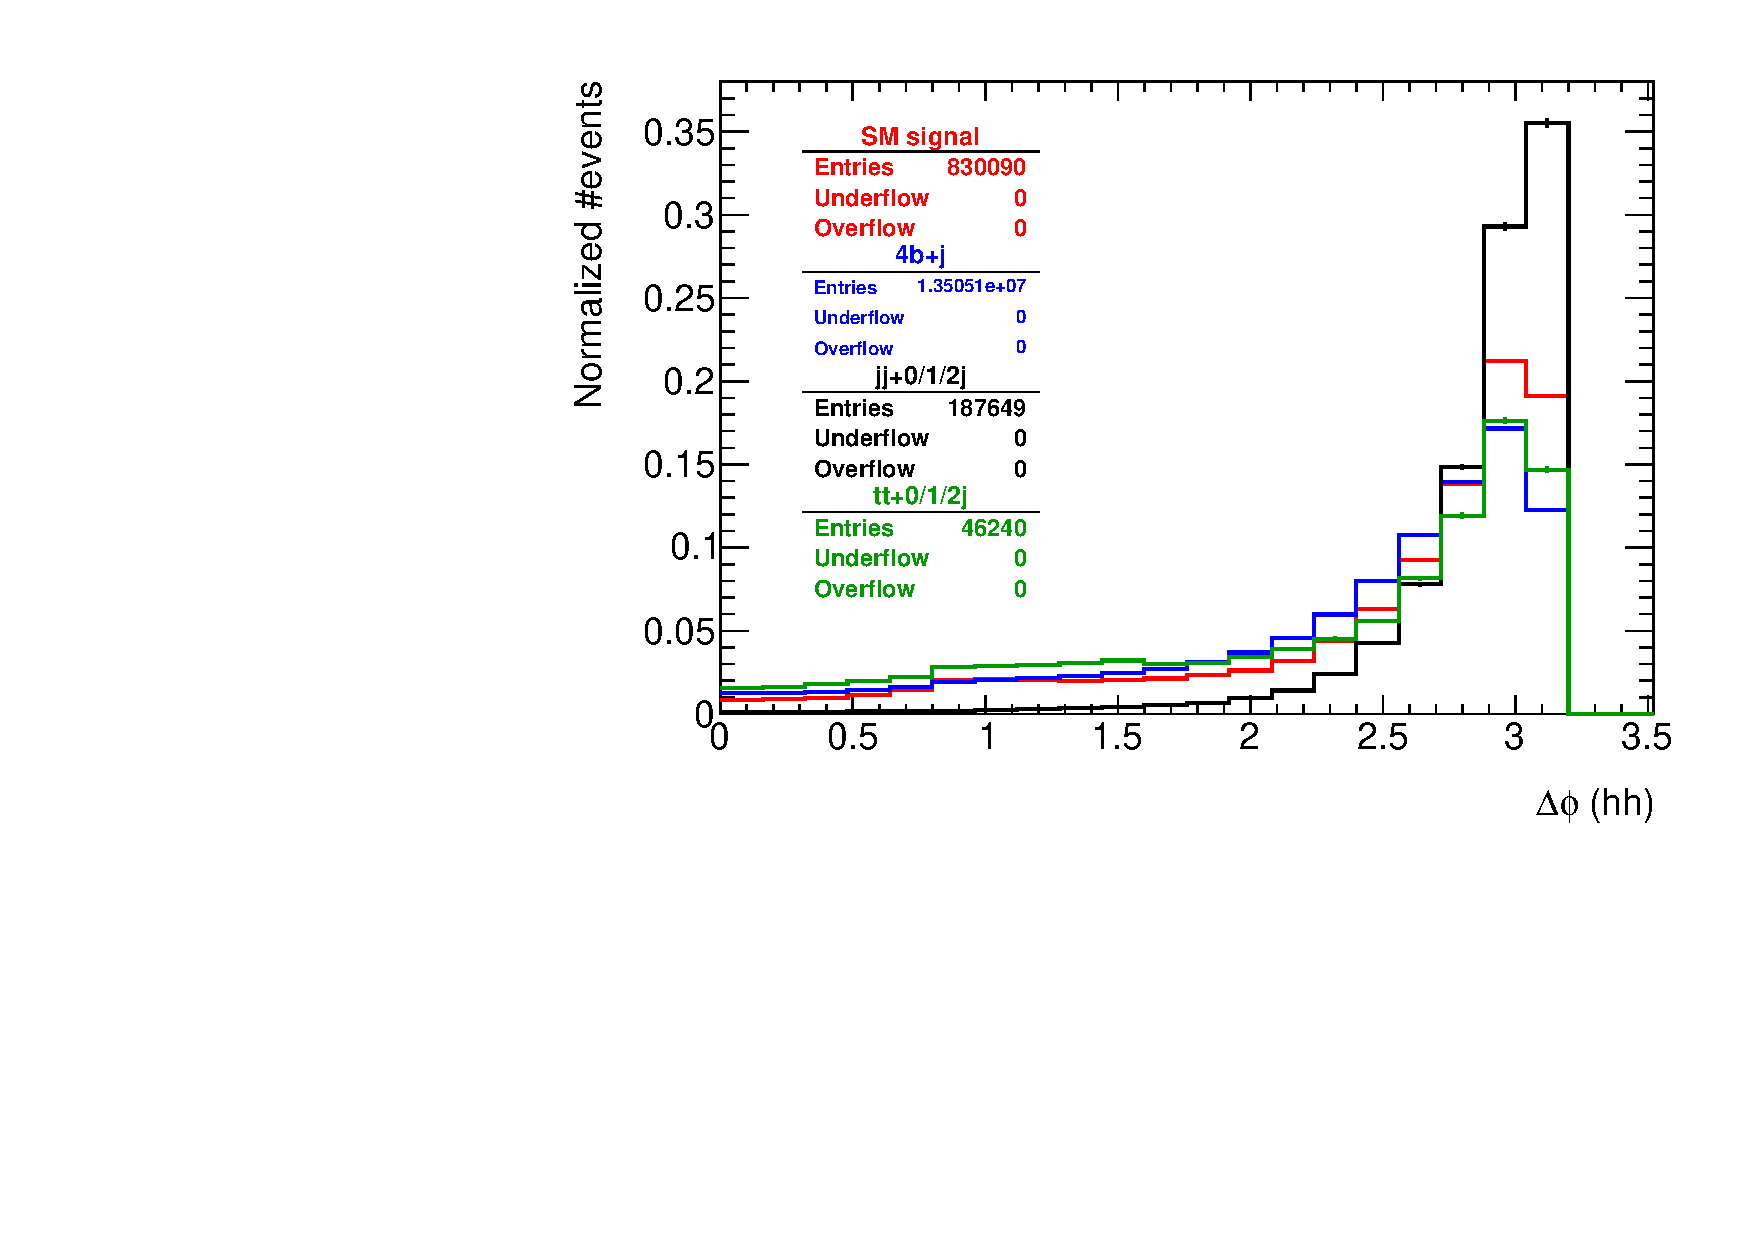
\includegraphics[width=\linewidth]{./Figures/hist_hh_deltaPhi.pdf}
		%\caption{$\Delta\phi$ between the Higgs candidates.}
		%\label{fig:deltaR_bb_pt}
	\end{minipage}%
	\begin{minipage}{.5\textwidth}
		\centering
		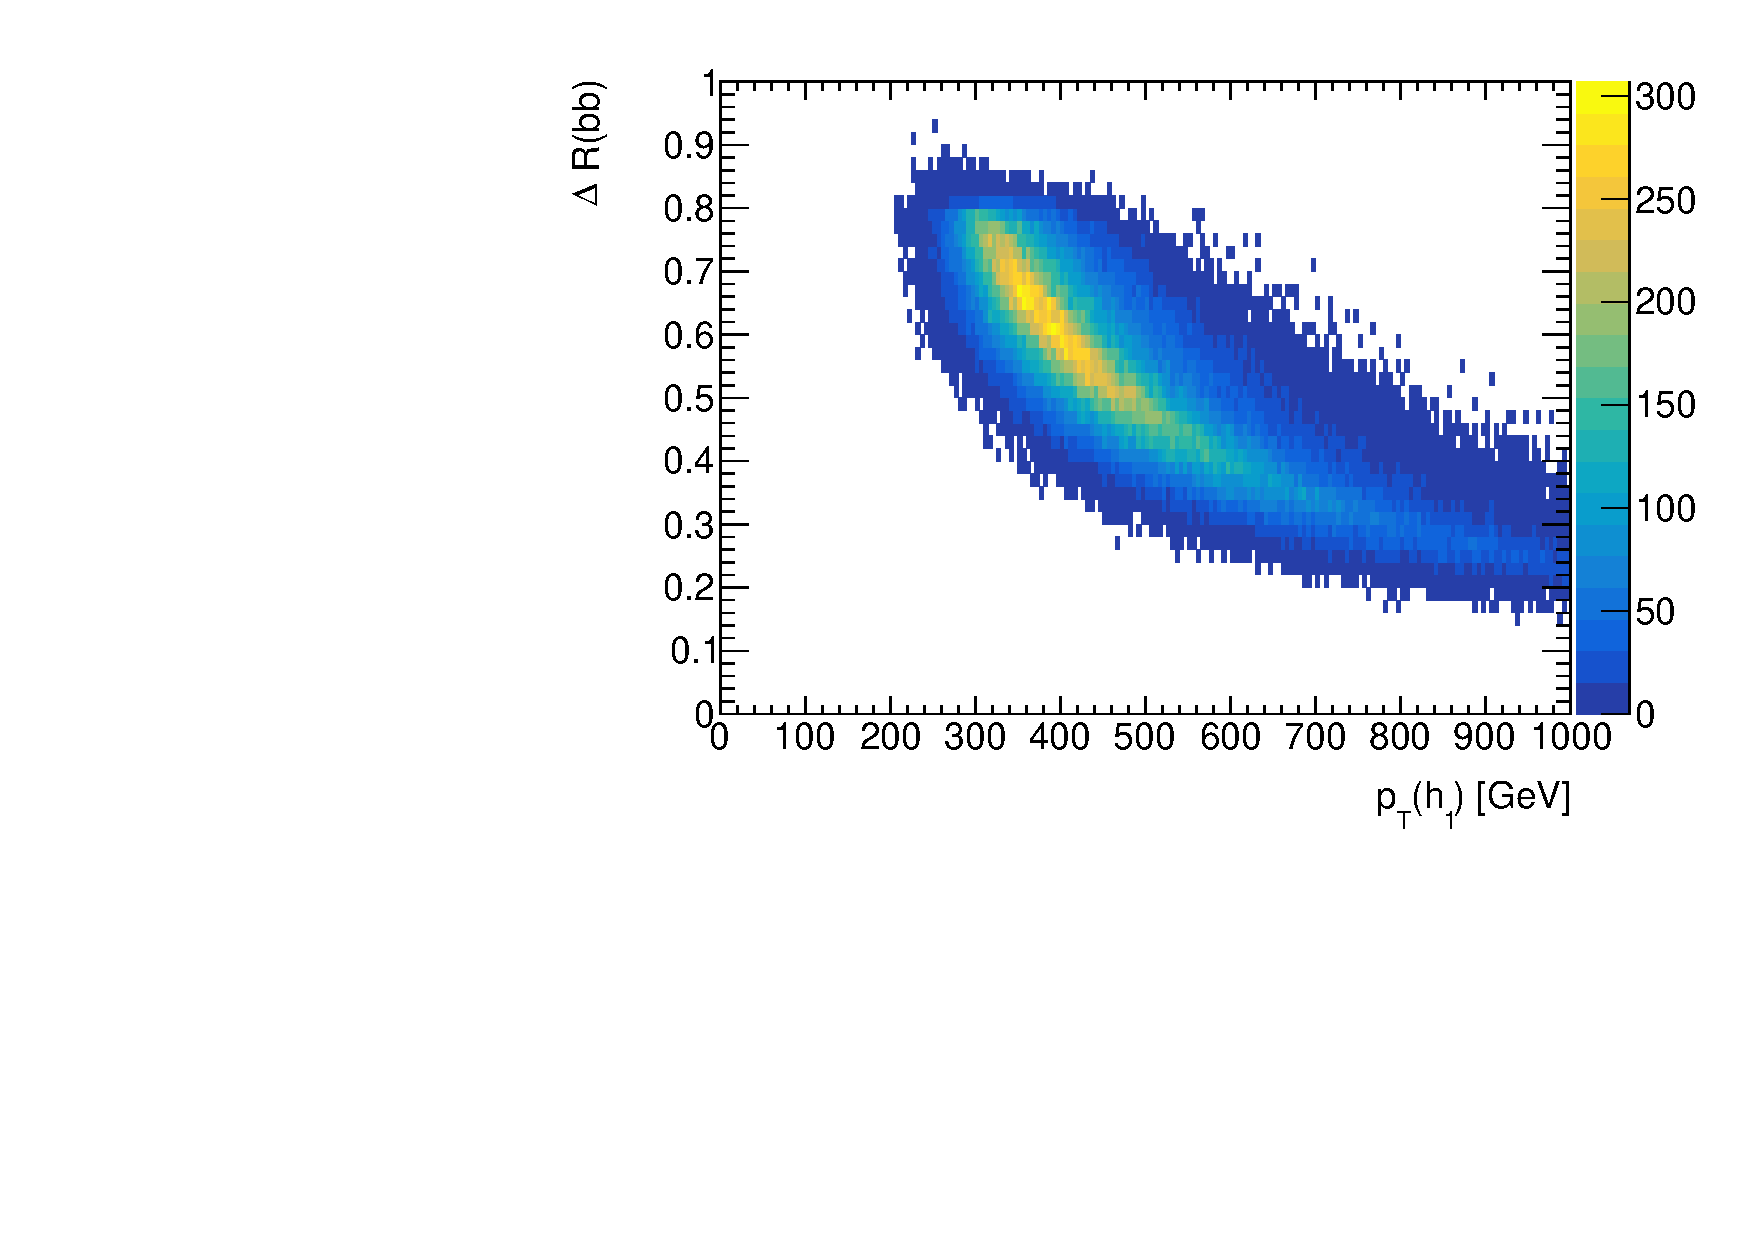
\includegraphics[width=\linewidth]{./Figures/hist_deltaR_bb_pt.pdf}
		%\label{fig:hh_deltaPhi}
		%\caption{$\Delta R$ between the b quarks coming from the decay of the leading Higgs candidate, $h_1$. To obtain this plot the cut $|M-125|<40$ GeV was applied in addition to the pre-selection cuts.}
	\end{minipage}
	\begin{minipage}[t]{0.5\textwidth}
		\caption*{(a)}
		%\label{fig1}
	\end{minipage}%%%
	\hfill
	\begin{minipage}[t]{0.5\textwidth}
		\caption*{(b)}
		%\label{fig2}
	\end{minipage}
	\caption{(a) $\Delta\phi$ between the Higgs candidates, $\Delta\phi(hh)$, (b) $\Delta R$ between the b quarks coming from the decay of the leading Higgs candidate, $h_1$, versus $p_T(h_1)$. To obtain this plot the cut $|M(h_1,h_2)-125|<40$ GeV was applied in addition to the pre-selection cuts.}
	\label{fig:deltaPhi_deltaR}
\end{figure}

%\begin{figure}
%	\centering
%	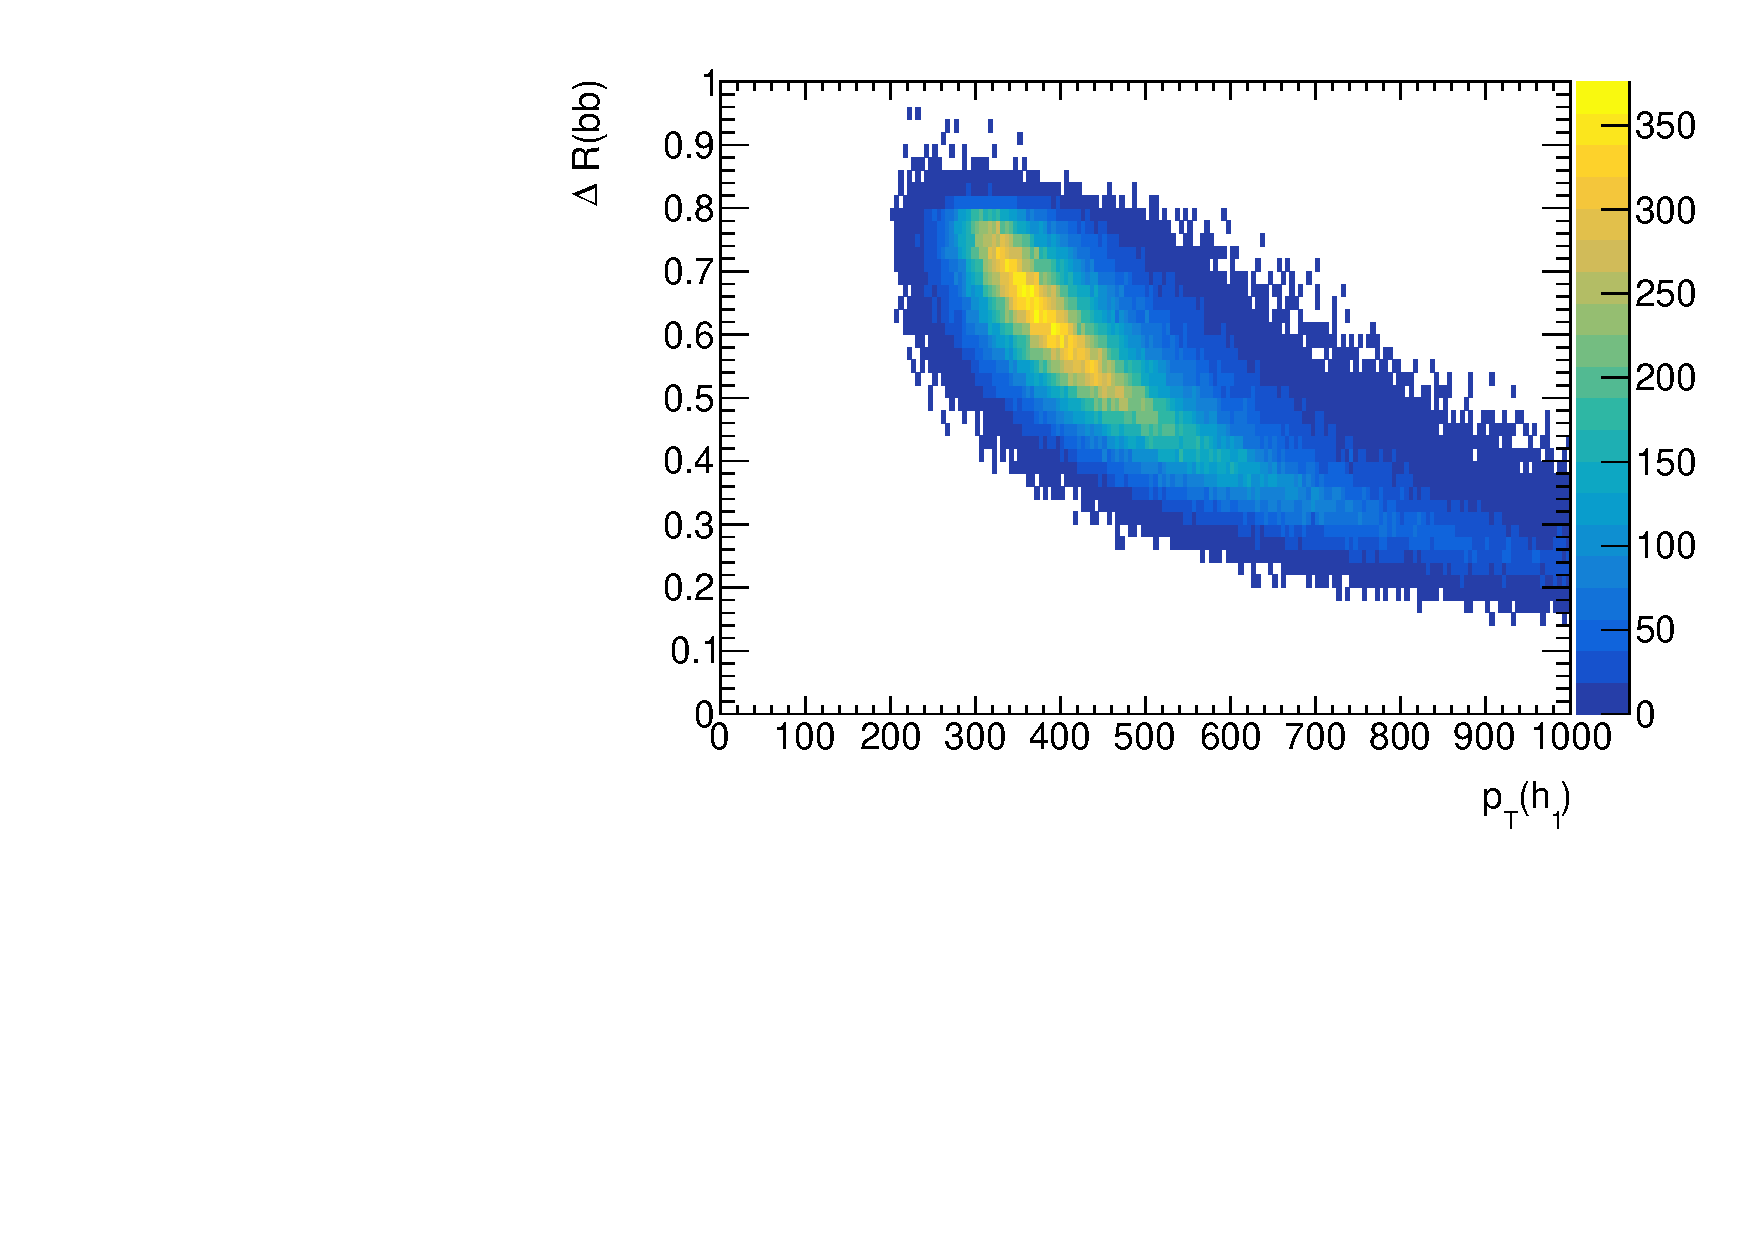
\includegraphics[width=0.7\linewidth]{./Figures/deltaR_bb_pt.pdf}
%	\label{fig:deltaR_bb_pt}
%	\caption{$\Delta R$ between the b quarks coming from the decay of the leading Higgs candidate, $h_1$. Plot obtained after the pre-selection cuts.}
%\end{figure}

%In the boosted regime, we expect at least two jets that are reconstructed using a large R parameter and that contain, each, the two b quarks that come from the decay of a Higgs boson. In the fully resolved regime, we expect at least four jets reconstructed with the standard R parameter of $0.4$, each corresponding to a b quark. Furthermore, an intermediate (or semi-resolved) category, in which one of the Higgs can be fully reconstructed using two small R jets and the other is reconstructed using a single large-R jet can also be explored. In all categories, we expect the presence of extra jets due to QCD activity. 

\subsection{Backgrounds}

The relevant backgrounds for this analysis are QCD multijet production, $t\overline{t}$ and $b\overline{b}b\overline{b}$. Although the $b\overline{b}b\overline{b}$ background is a particular case of a QCD multijet production process we consider it separately because it constitutes the irreducible background and therefore will have a higher efficiency in the analysis. The cross sections for these processes are several orders of magnitude larger than the cross section for the signal, as shown in table \ref{table:samples_summary}. In addition, in the case of the $t\overline{t}$ background, the event topology is expected to be similar to the signal because it also consists in the production of a pair of particles with the same mass.

The assumption that QCD multijet production and $t\overline{t}$ are the two main backgrounds is corroborated by the ATLAS di-Higgs search performed in the same channel \cite{hh2bbbbATLAS}, where these backgrounds were found to be the dominant ones. All other sources of backgrounds, including processes involving Higgs bosons, are found to be negligible. In appendix \ref{chapter:bkgHiggs} we discuss and evaluate the importance of some backgrounds that include Higgs bosons in our analysis.

Figure \ref{fig:QCD} shows examples of LO Feynman diagrams that contribute to $4b+~j$ (left), three- (middle) and four-light (right) jets production. The $b\overline{b}b\overline{b}$ background is generated with an extra light jet at generator level, as discussed in chapter \ref{chapter:tools}. This jet has a minimum $p_T$ of $200$ GeV, which means the the vector sum of the $p_T$ of the four b quarks must also be above $200$ GeV in order to conserve momentum. This increases the probability of two b quarks being reconstructed as single large-$R$ jet therefore emulating the signal's final state signature, i.e, high $p_T$ jets compatible with a two-prong substructure. The QCD $4b+j$ sample with $(200<p_T<500)$ GeV has a cross section of approximately $756$ pb. In addition, as explained in section \ref{sec:Pythia_samples}, we multiply this cross section by a k-factor of $2$, which yields a total cross section of approximately $1.5\times 10^{3}$ pb. The cross section is a lot smaller for the other $4b+j$ QCD sample as well as for the samples that include both QCD and eletroweak contributions, as expected.

The QCD multijet background consists of two, three and four jet events (represented as $jj+0/1/2 ~j$), at generator level. The jets can originate from light and b quarks and from gluons. A jet matching procedure is implemented in Pythia in order to avoid double counting. Due to non-zero mistagging probabilities, light and c jets can be identified as b jets. Although these probabilities are relatively small when compared to the b-tagging efficiency (see section \ref{sec:btagging}) the cross section of multijet processes is very large, such that this background becomes dominant. The $jj+0/1/2 ~j$ sample with $(500<H_T<1000)$ GeV has a cross section of the order of $10^7$ pb. As anticipated, the $p_T$ spectrum of the multijet background is a lot softer than that of the signal and remaining backgrounds, as is shown in figures \ref{fig:h1h2_pt}(a) and \ref{fig:h1h2_pt}(b). In addition, for this background the $\tau_{21}$ variable takes values close to one, as it is shown in figure \ref{fig:hh_deltaEta_h1_tau21}(b). This indicates that the jets are not consistent with containing two subjets. 

Figure \ref{fig:tt} shows examples of LO Feynman diagrams that contribute to $t\overline{t}$ production through $q\overline{q}$ (left) and $gg$ (middle and right) fusion. The $t\overline{t}$ background is simulated with additional zero, one or two jets (represented as $t\overline{t}+0/1/2 ~j$), at generator level. The extra jets can originate from light, c or b quarks or from gluons. A jet matching procedure is implemented in Pythia in order to avoid double counting. The top quark has a very short lifetime, predicted to be $5\times 10^{-25}$ s, such that it decays before it can hadronize. This sample is inclusive in the top quark decay modes. However, the most favoured decay of the top quark is $t\rightarrow Wb$ with a branching ratio close to $96\%$ \cite{PDG2016}. Therefore, $t\overline{t}$ events will, most of the time, result in the $W^+W^-b\overline{b}$ final state. We do not specify any decay mode for the $W$ such that the sample is also inclusive in the $W$ decay modes. The $W$ decays to hadrons $(W^+\rightarrow q\overline{q})$ and leptons $(W^+\rightarrow l^+\nu)$ with BR$(W^+\rightarrow q\overline{q})\sim 68\%$ and BR$(W^+\rightarrow l^+\nu)\sim 10\%$. If one (or both) $W$ bosons decays to hadrons then there will be additional jets in the final state. These can be b initiated jets (although the probability is very small) or can be light jets misidentified as b jets. If both $W$ bosons decay to leptons there will still be at least two b jets in the final state, coming from the $t\overline{t}$ decay. The cross section of the $t\overline{t}+0/1/2 ~j$ is approximately $4.3\times 10^4$ pb. As explained in \ref{sec:Pythia_samples}, a k-factor of $1.74$ is applied which yields a total cross section of approximately $7.5\times 10^{4}$ pb.

It is interesting to note that in the softdrop mass distribution for the leading Higgs candidate (figure \ref{fig:h1_eta_M}(b)) the $t\overline{t}$ background (green line) shows a small peak at around $170$ GeV. In this region, all the decay products of the top quark are contained inside the $R=0.8$ jet such that the jet mass corresponds to the mass of the original top quark.

%In addition, we also take into account the irreducible background, $b\overline{b}b\overline{b}$ because it is expected to be the background with the highest efficiency.

%	\feynmandiagram[small,layered layout,horizontal=a to b] {
%		%{[edges=fermion] a -- b -- c,}
%		{ [same layer, edges=anti fermion] a -- a1 -- c},
%		i1 [particle=\(\overline{q}\)]-- [anti fermion] a-- [boson]  b,
%		a1-- [gluon] d [particle=\(g\)] ,
%		i3 [particle=\(q\)]-- [fermion] c -- [boson] e ,
%		% Draw the two internal fermion lines		
%		%{ [  same layer] c -- [anti fermion] e},
%		%f1  -- [fermion] b -- [fermion] f2 ,
%		%f3  -- [fermion] f2 -- [gluon] g1 ,
%		%f4  -- [fermion] g1 -- [fermion] f5 ,
%		%	a -- [opacity=0.2] c,
%		%g1 -- [anti fermion] b,
%		e -- [anti fermion] f2 [particle=\(\overline{b}\)],
%		e -- [fermion] f3 [particle=\(b\)],
%		b -- [fermion] k [particle=\(\overline{b}\)],
%		b -- [anti fermion] j [particle=\(b\)],
%	};

\begin{figure}
	\centering
%	\feynmandiagram[small,layered layout,horizontal=i1 to a] {% Draw the top and bottom lines
%		i1 [particle=\(\overline{q}\)]-- [anti fermion] a-- [boson, edge label'=\(g/h/Z/\gamma\)]  b,
%		i2 [particle=\(q\)]-- [fermion] c-- [gluon, edge label=\(g\)] d,
%		% Draw the two internal fermion lines
%		{ [  same layer] a -- [anti fermion] c},
%		%f1  -- [fermion] b -- [fermion] f2 ,
%		%f3  -- [fermion] f2 -- [gluon] g1 ,
%		%f4  -- [fermion] g1 -- [fermion] f5 ,
%		%	a -- [opacity=0.2] c,
%		%g1 -- [anti fermion] b,
%		b -- [anti fermion] f2 [particle=\(\overline{b}\)],
%		b -- [fermion] f3 ,
%		f3 -- [fermion] f4 [particle=\(b\)],
%		f3 -- [boson, edge label'=\(g/h/Z/\gamma\)] g1,
%		g1 -- [anti fermion] f5 [particle=\(\overline{b}\)],
%		g1 -- [fermion] f6 [particle=\(b\)],
%	};\qquad
%	\feynmandiagram[small,layered layout,horizontal=a to b] {
%		%{[edges=fermion] a -- b -- c,}
%		{ [same layer, edges=anti fermion] a -- a1 -- c},
%		i1 [particle=\(\overline{q}\)]-- [anti fermion] a-- [boson]  b,
%		a1-- [gluon] d [particle=\(g\)] ,
%		i3 [particle=\(q\)]-- [fermion] c -- [boson] e ,
%		% Draw the two internal fermion lines		
%		%{ [  same layer] c -- [anti fermion] e},
%		%f1  -- [fermion] b -- [fermion] f2 ,
%		%f3  -- [fermion] f2 -- [gluon] g1 ,
%		%f4  -- [fermion] g1 -- [fermion] f5 ,
%		%	a -- [opacity=0.2] c,
%		%g1 -- [anti fermion] b,
%		e -- [anti fermion] f2 [particle=\(\overline{b}\)],
%		e -- [fermion] f3 [particle=\(b\)],
%		b -- [fermion] k [particle=\(\overline{b}\)],
%		b -- [anti fermion] j [particle=\(b\)],
%	};\quad
	\begin{tikzpicture}
	\begin{feynman}
	\vertex (b);
	\vertex [below=of b] (c);
	\vertex [above=of b] (a);
	\vertex [left=of a] (i1) {\(q\)};
	\vertex [left=of c] (i2) {\(\overline{q}\)};
	\vertex [right=of a] (f1);
	\vertex [right=of b] (f2) {\(g\)};
	\vertex [right=of c] (f3);
	\vertex [above right=1cm and 1.4cm of f1] (i3) {\(b\)};
	\vertex [below right=1cm and 1.4cm of f1] (i4) {\(\overline{b}\)};
	\vertex [above right=1cm and 1.4cm of f3] (i5) {\(b\)};
	\vertex [below right=1cm and 1.4cm of f3] (i6) {\(\overline{b}\)};
	
	\diagram* {
		(a) -- [fermion] (b) -- [fermion] (c),
		(i1) -- [fermion] (a),
		(i2) -- [anti fermion] (c),
		(a) -- [boson, edge label'=\(g/h/Z/\gamma\)] (f1),
		(b) -- [boson, edge label'=\(g/h/Z/\gamma\)] (f2),
		(c) -- [boson, edge label'=\(g/h/Z/\gamma\)] (f3),
		(f1) -- [fermion] (i3)
		(f1) -- [anti fermion] (i4),
		(f3) -- [fermion] (i5),
		(f3) -- [anti fermion] (i6),
	};
	
	\end{feynman}
	\end{tikzpicture}\qquad
	\feynmandiagram[small,layered layout,horizontal=a to b] {% Draw the top and bottom lines
		i1 [particle=\(\overline{q}\)]-- [anti fermion] a-- [anti fermion]  b,
		i2 [particle=\(q\)]-- [fermion] c-- [fermion] d [particle=\(q\)],
		% Draw the two internal fermion lines
		{ [  same layer] a -- [gluon] c},
		%f1  -- [fermion] b -- [fermion] f2 ,
		%f3  -- [fermion] f2 -- [gluon] g1 ,
		%f4  -- [fermion] g1 -- [fermion] f5 ,
		%	a -- [opacity=0.2] c,
		%g1 -- [anti fermion] b,
		b -- [anti fermion] f2 [particle=\(\overline{q}\)],
		b -- [gluon] f3 [particle=\(g\)],
	};\qquad
	\feynmandiagram
	[horizontal=a to b] {i1 [particle=\(q\)] -- [fermion] a -- [fermion] i2 [particle=\(\overline{q}\)],
		a -- [gluon] b,
		g1 -- [gluon] b -- [gluon] g2,
		f1 [particle=\(\overline{q}\)] -- [fermion] g1 -- [fermion] f2 [particle=\(q\)],
		f3 [particle=\(\overline{q}\)] -- [fermion] g2 -- [fermion] f4 [particle=\(q\)],
		g1 -- [opacity=0] g2,
		f2 -- [opacity=0] f4,
	};
%			\feynmandiagram[small,layered layout,horizontal=i1 to a] {% Draw the top and bottom lines
%				i1 [particle=\(\overline{q}\)]-- [anti fermion] a-- [boson, edge label'=\(h/Z/\gamma\)]  b,
%				i2 [particle=\(q\)]-- [fermion] c-- [gluon, edge label=\(g\)] d,
%				% Draw the two internal fermion lines
%				{ [  same layer] a -- [anti fermion] c},
%				%f1  -- [fermion] b -- [fermion] f2 ,
%				%f3  -- [fermion] f2 -- [gluon] g1 ,
%				%f4  -- [fermion] g1 -- [fermion] f5 ,
%				%	a -- [opacity=0.2] c,
%				%g1 -- [anti fermion] b,
%				b -- [anti fermion] f2 [particle=\(\overline{b}\)],
%				b -- [fermion] f3 ,
%				f3 -- [fermion] f4 [particle=\(b\)],
%				f3 -- [boson, edge label'=\(h/Z/\gamma\)] g1,
%				g1 -- [anti fermion] f5 [particle=\(\overline{b}\)],
%				g1 -- [fermion] f6 [particle=\(b\)],
%			};
	\caption{Example of diagrams that contribute to the QCD multijet background: five final state jets, four of which are b-jets (left), three final state jets (middle) and four final state jets (right). Here, $q$ stands for a light quark/jet.}
	\label{fig:QCD}
\end{figure}

\begin{figure}
\centering
\feynmandiagram
[horizontal=a to b] {i1 [particle=\(q\)] -- [fermion] a -- [fermion] i2 [particle=\(\overline{q}\)],a -- [gluon,edge label=\(g\)] b, f1 [particle=\(t\)] -- [fermion] b -- [fermion] f2 [particle=\(\overline{t}\)],
};\qquad
\feynmandiagram
[horizontal=a to b] {i1 [particle=\(g\)] -- [gluon] a -- [gluon] i2 [particle=\(g\)],a -- [gluon,edge label=\(g\)] b, f1 [particle=\(t\)] -- [fermion] b -- [fermion] f2 [particle=\(\overline{t}\)],
}; \qquad
\feynmandiagram[layered layout,horizontal=a to b] {% Draw the top and bottom lines
	i1 [particle=\(g\)]-- [gluon] a-- [anti fermion]  b [particle=\(\overline{t}\)] -- ,i2 [particle=\(g\)]-- [gluon] c-- [fermion] d [particle=\(t\)] -- ,
	% Draw the two internal fermion lines
	{ [  same layer] a -- [fermion] c},
};
\caption{Dominant diagrams of $pp\rightarrow t\overline{t}$ at LO.}
\label{fig:tt}
\end{figure}


%\begin{figure}[h]
%	\centering
%	\feynmandiagram [horizontal=b to c] {
%		a -- [gluon] b [blob],c -- [scalar] b-- [gluon] d,
%		c -- [scalar] e,
%		c -- [scalar] f,
%		e -- [fermion] g,
%		e -- [anti fermion] h,
%		f -- [fermion] i,
%		f -- [anti fermion] j,
%	};
%	\caption{Final state}
%\end{figure}

%\begin{figure}[h]
%	\centering
%	\feynmandiagram [horizontal=d to h] {
%		a [particle=\(g\)] -- [gluon] b [blob],
%		c [particle=\(g\)] -- [gluon] b -- [gluon],
%		d -- [scalar, edge label'=\(h\)] b -- [scalar],
%		e -- [scalar, edge label'=\(h\)] b -- [scalar],
%		d -- [fermion, edge label=\(b\)] g ,
%		d -- [anti fermion, edge label=\(\overline{b}\)] h ,
%		e -- [fermion, edge label'=\(b\)] i,
%		e -- [anti fermion, edge label'=\(\overline{b}\)] j ,
%		d -- [opacity=0] e,
%		%h -- [opacity=0] i,
%		g -- [opacity=0] h,
%		i -- [opacity=0] j,
%		h -- [opacity=0] i,
%	};
%	\caption{Final state}
%\end{figure}




%\begin{table}
%	\centering
%	\begin{tabular}{lp{30mm}p{10mm}p{30mm}p{30mm}}
%		\toprule 
%		Pythia & hh (h$\rightarrow b\overline{b}$) & 4b+j & jj+0/1/2 j & tt+0/1/2 j \\
%		\midrule
%		Relevant settings & 25:onMode=off \newline 25:onIfAny= 5 -5&  & \textbf{Jet matching:} \newline merge=on \newline scheme=1 \newline setMad=off \newline coneRadius=1.0 \newline etaJetMax=10 \newline nJetMax=4 \newline qCut=30 & \textbf{Jet matching:} \newline merge=on \newline scheme=1 \newline setMad=off \newline coneRadius=1.0 \newline etaJetMax=10 \newline nJetMax=2 \newline qCut=60\\
%		\rowcolor{black!7} Description & Turn on the $h\rightarrow b\overline{b}$ decay for the undecayed Higgs. &  &  \multicolumn{2}{l}{Set parameters for jet matching procedure. } \\
%		\bottomrule
%	\end{tabular}
%	\caption{oi}
%	\label{table:DelphesHCAL}
%\end{table}

\begin{figure}
	\centering
	\begin{minipage}{.5\textwidth}
		\centering
		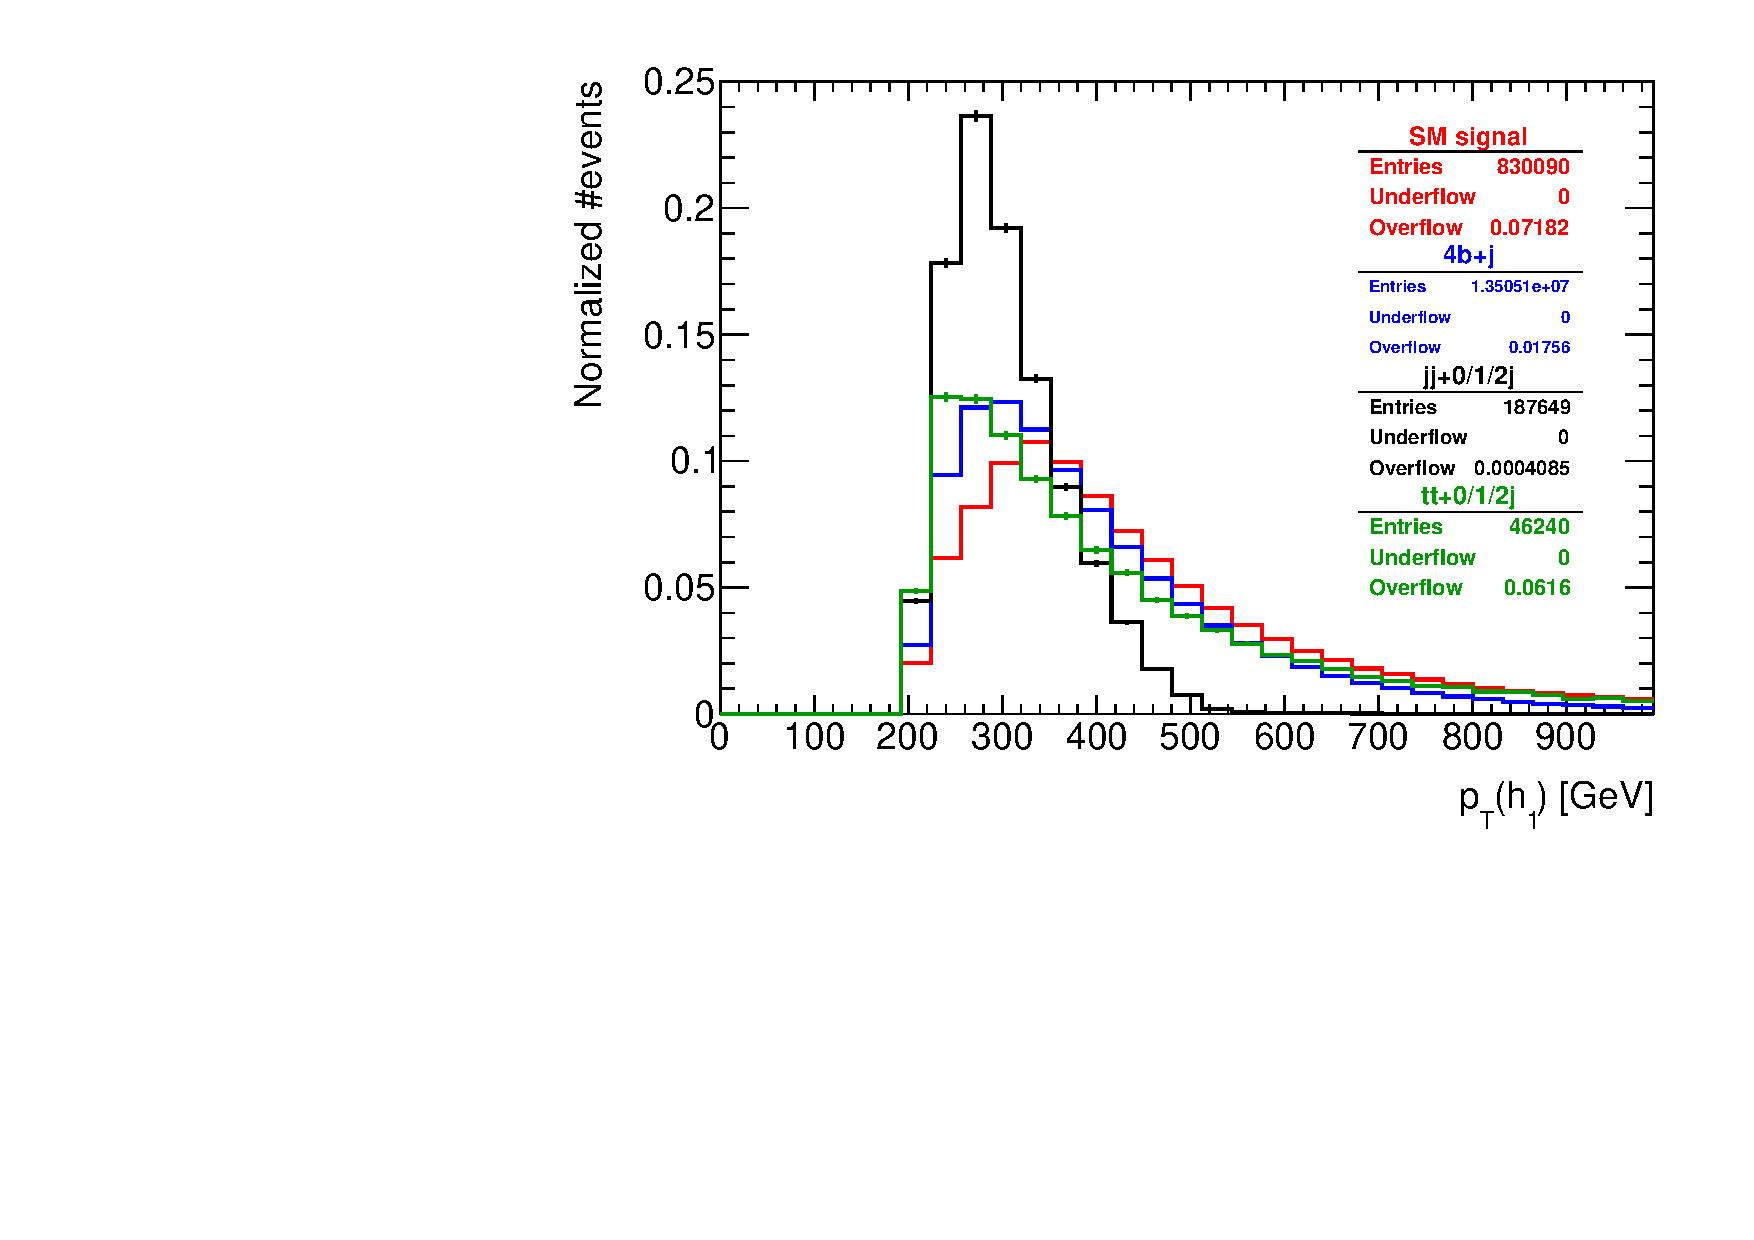
\includegraphics[trim={.65cm 0 0 0},clip,width=\linewidth]{./Figures/hist_h1_pt.pdf}
		%\caption{oi}
		%\label{fig:h1_pt}
	\end{minipage}%
	\begin{minipage}{.5\textwidth}
		\centering
		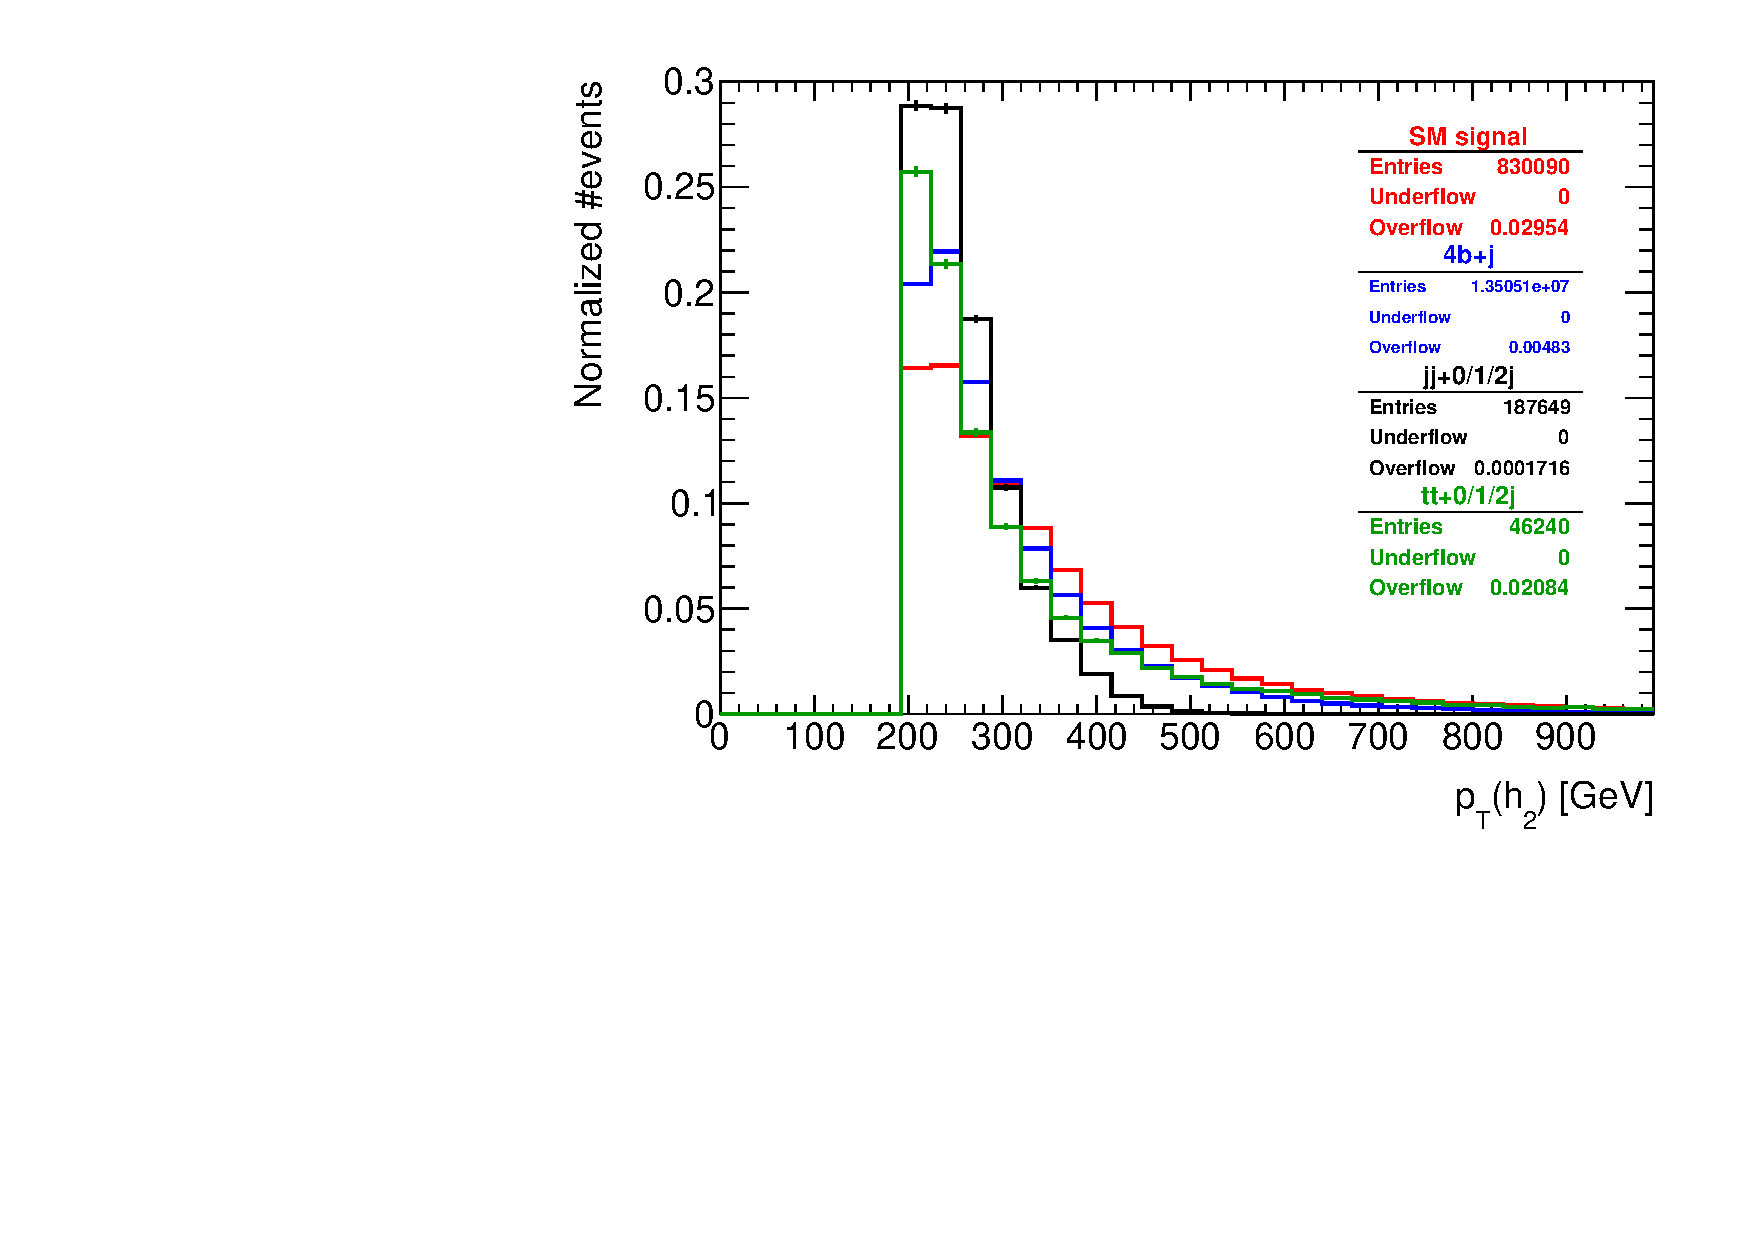
\includegraphics[trim={0 0 .65cm 0},clip,width=\linewidth]{./Figures/hist_h2_pt.pdf}
		%\caption{oi}
		%\label{fig:h2_pt}
	\end{minipage}
	\begin{minipage}[t]{0.5\textwidth}
		\caption*{(a)}
		%\label{fig1}
	\end{minipage}%%%
	\hfill
	\begin{minipage}[t]{0.5\textwidth}
		\caption*{(b)}
		%\label{fig2}
	\end{minipage}
	\caption{$p_T$ distributions for the leading (a) and sub leading (b) Higgs candidates. The signal is the SM $hh\rightarrow b\overline{b}$ process. The histograms are normalized to unit area and include all events that pass the pre-selection cuts.}
	\label{fig:h1h2_pt}
\end{figure}

\begin{figure}
	\centering
	\begin{minipage}{.5\textwidth}
		\centering
		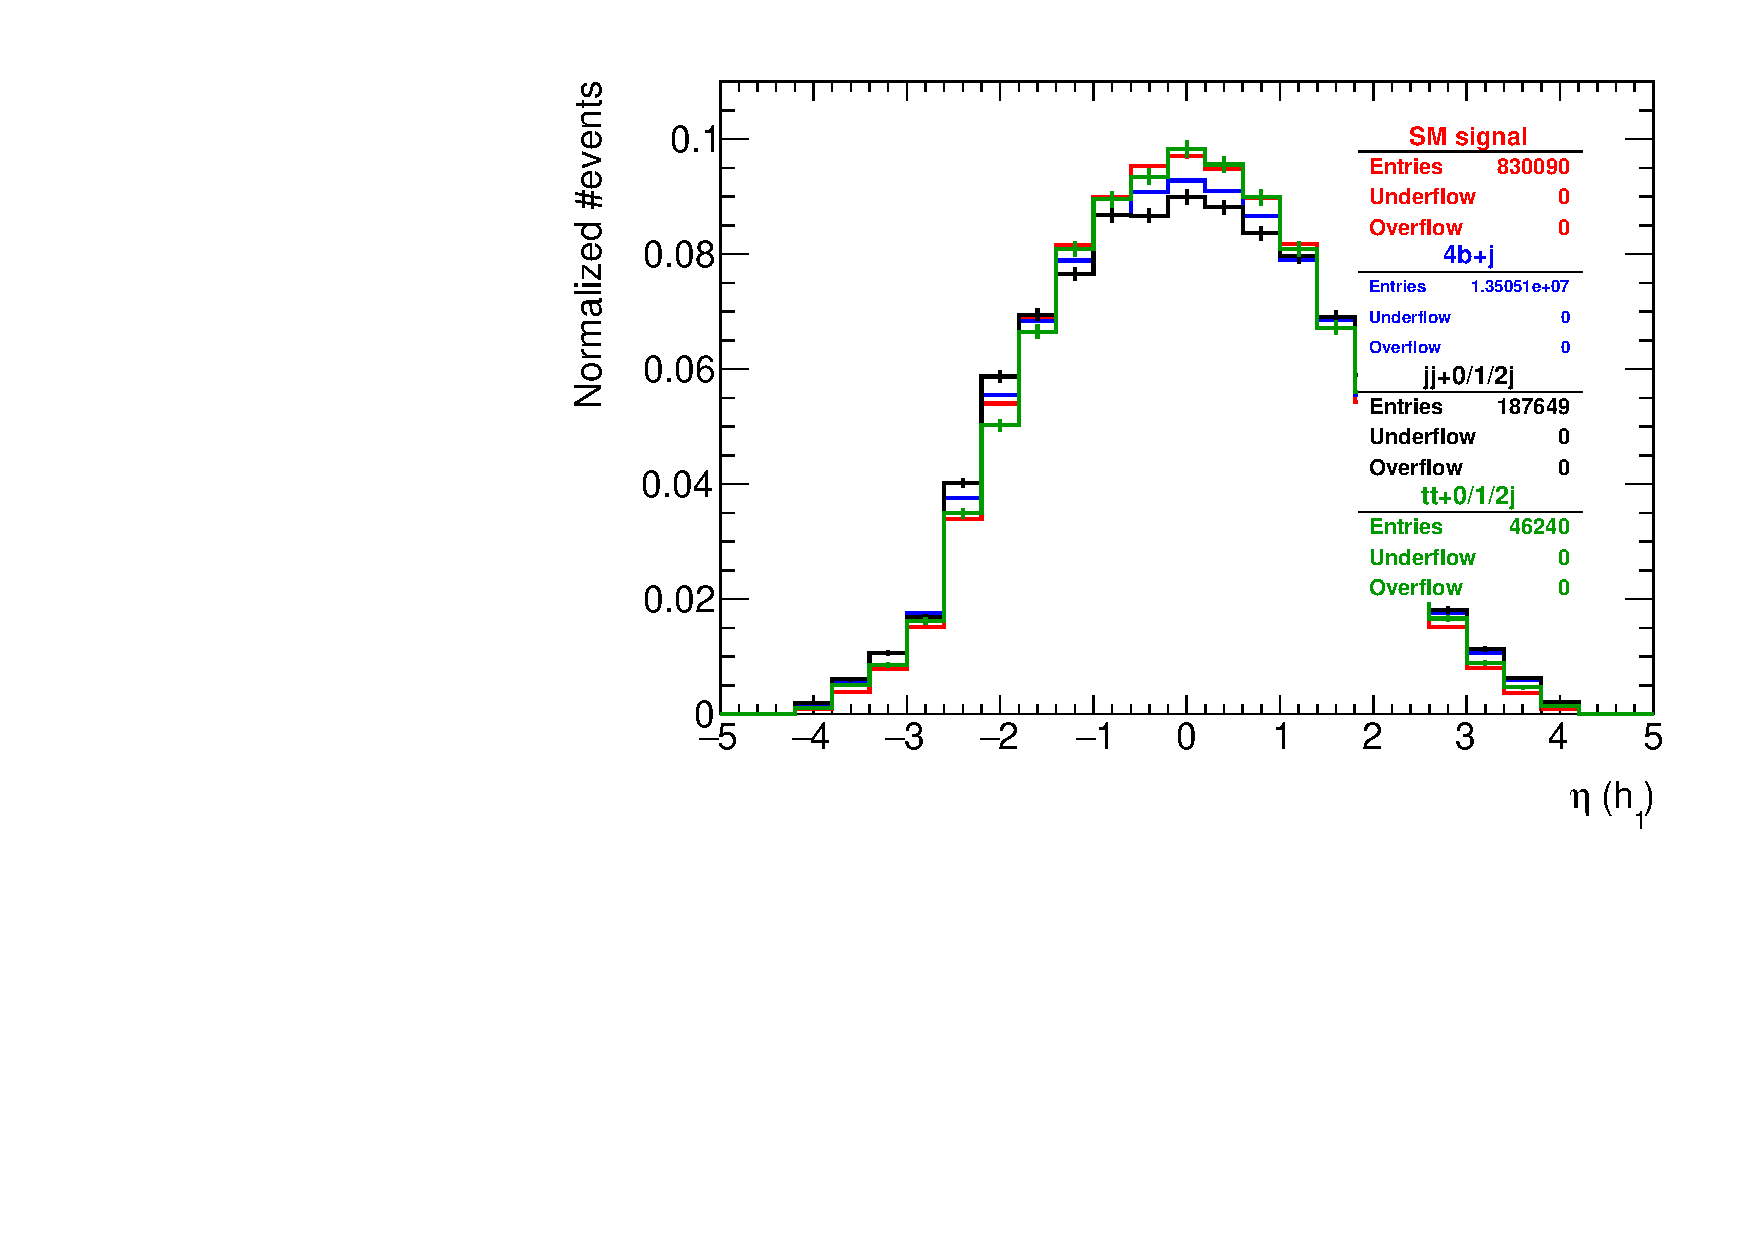
\includegraphics[trim={.65cm 0 0 0},clip,width=\linewidth]{./Figures/hist_h1_eta.pdf}
		%\caption{oi}
		%\label{fig:h1_pt}
	\end{minipage}%
	\begin{minipage}{.5\textwidth}
		\centering
		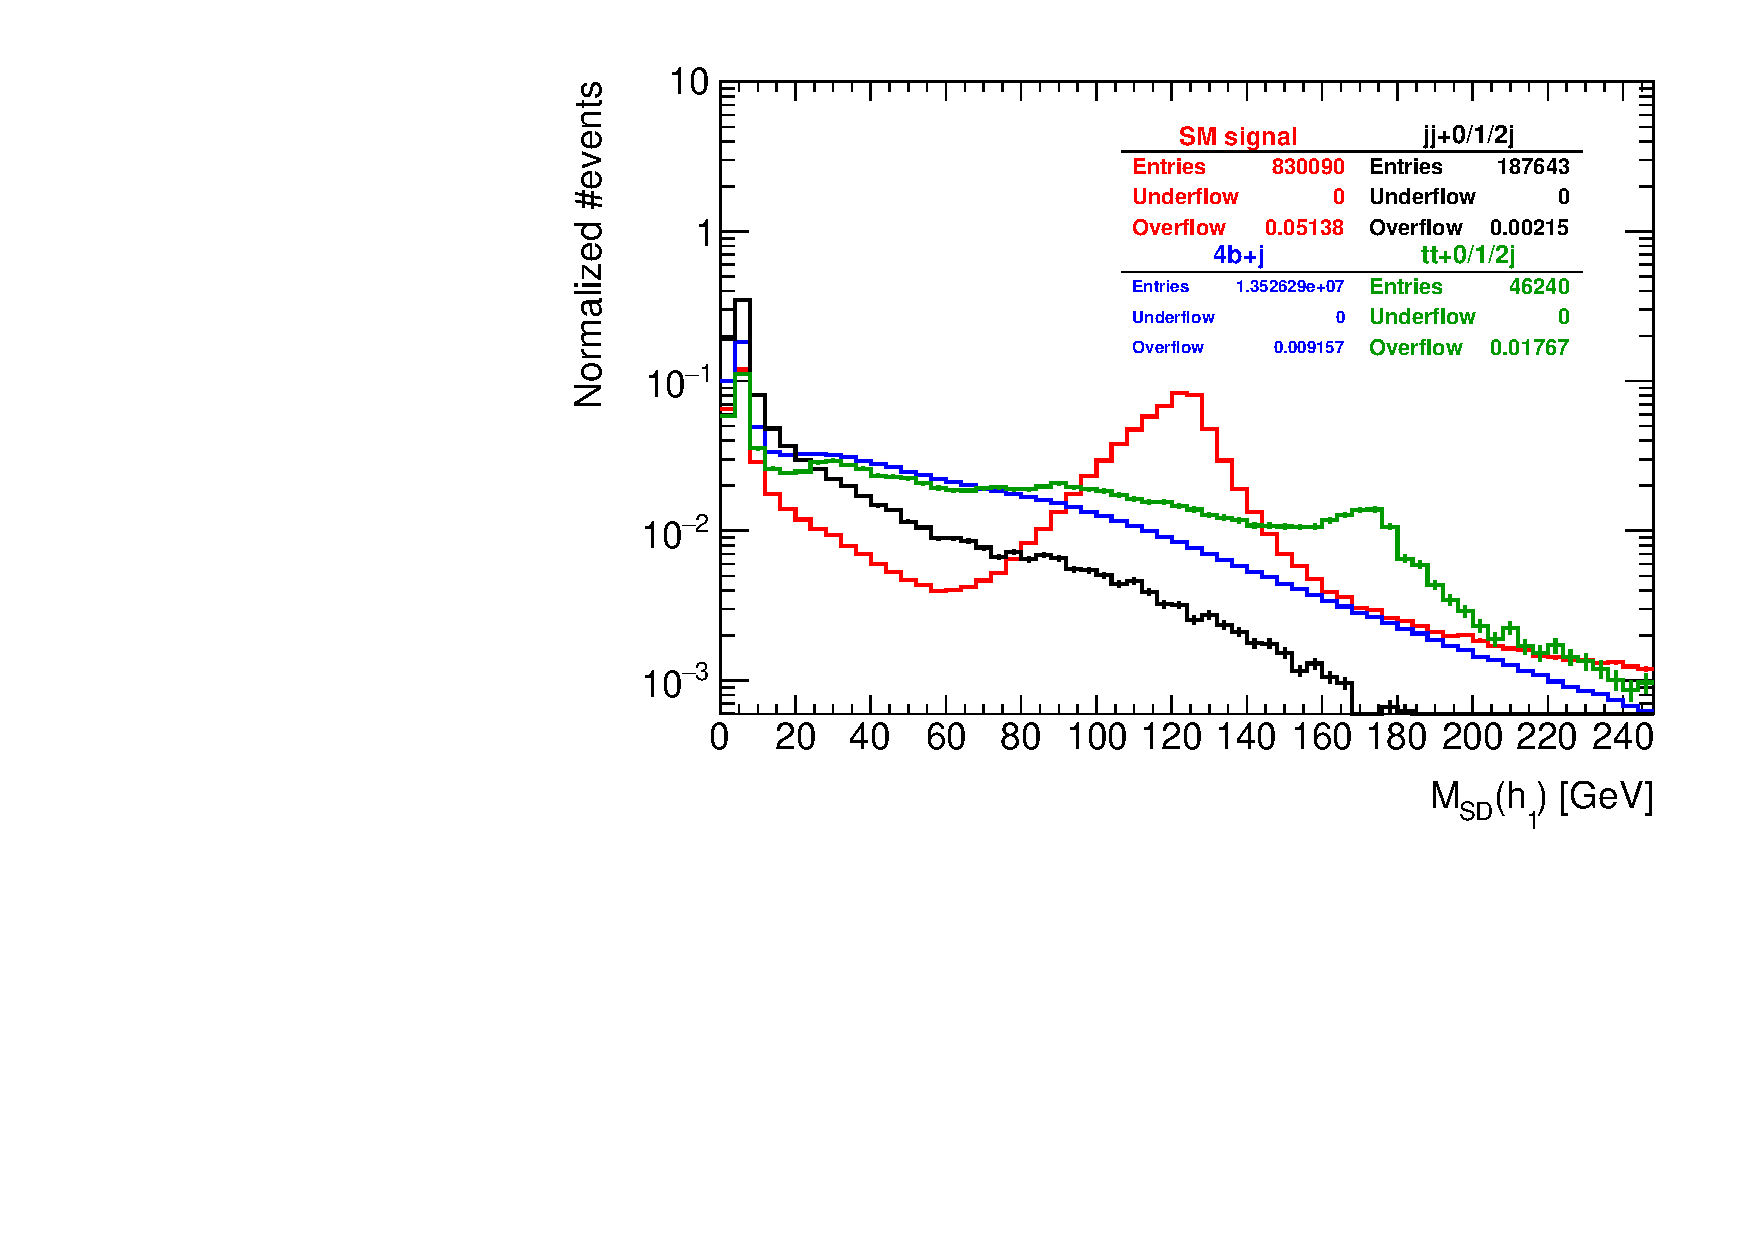
\includegraphics[trim={0 0 .65cm 0},clip,width=\linewidth]{./Figures/hist_h1_softdrop_M.pdf}
		%\caption{oi}
		%\label{fig:h2_pt}
	\end{minipage}
	\begin{minipage}[t]{0.5\textwidth}
		\caption*{(a)}
		%\label{fig1}
	\end{minipage}%%%
	\hfill
	\begin{minipage}[t]{0.5\textwidth}
		\caption*{(b)}
		%\label{fig2}
	\end{minipage}
	\caption{$\eta$ (a) and softdrop mass (b) distributions for the leading Higgs candidate. The signal is the SM $hh\rightarrow b\overline{b}$ process. The histograms are normalized to unit area and include all events that pass the pre-selection cuts.}
	\label{fig:h1_eta_M}
\end{figure}	

\begin{figure}
	\centering
	\begin{minipage}{.5\textwidth}
		\centering
		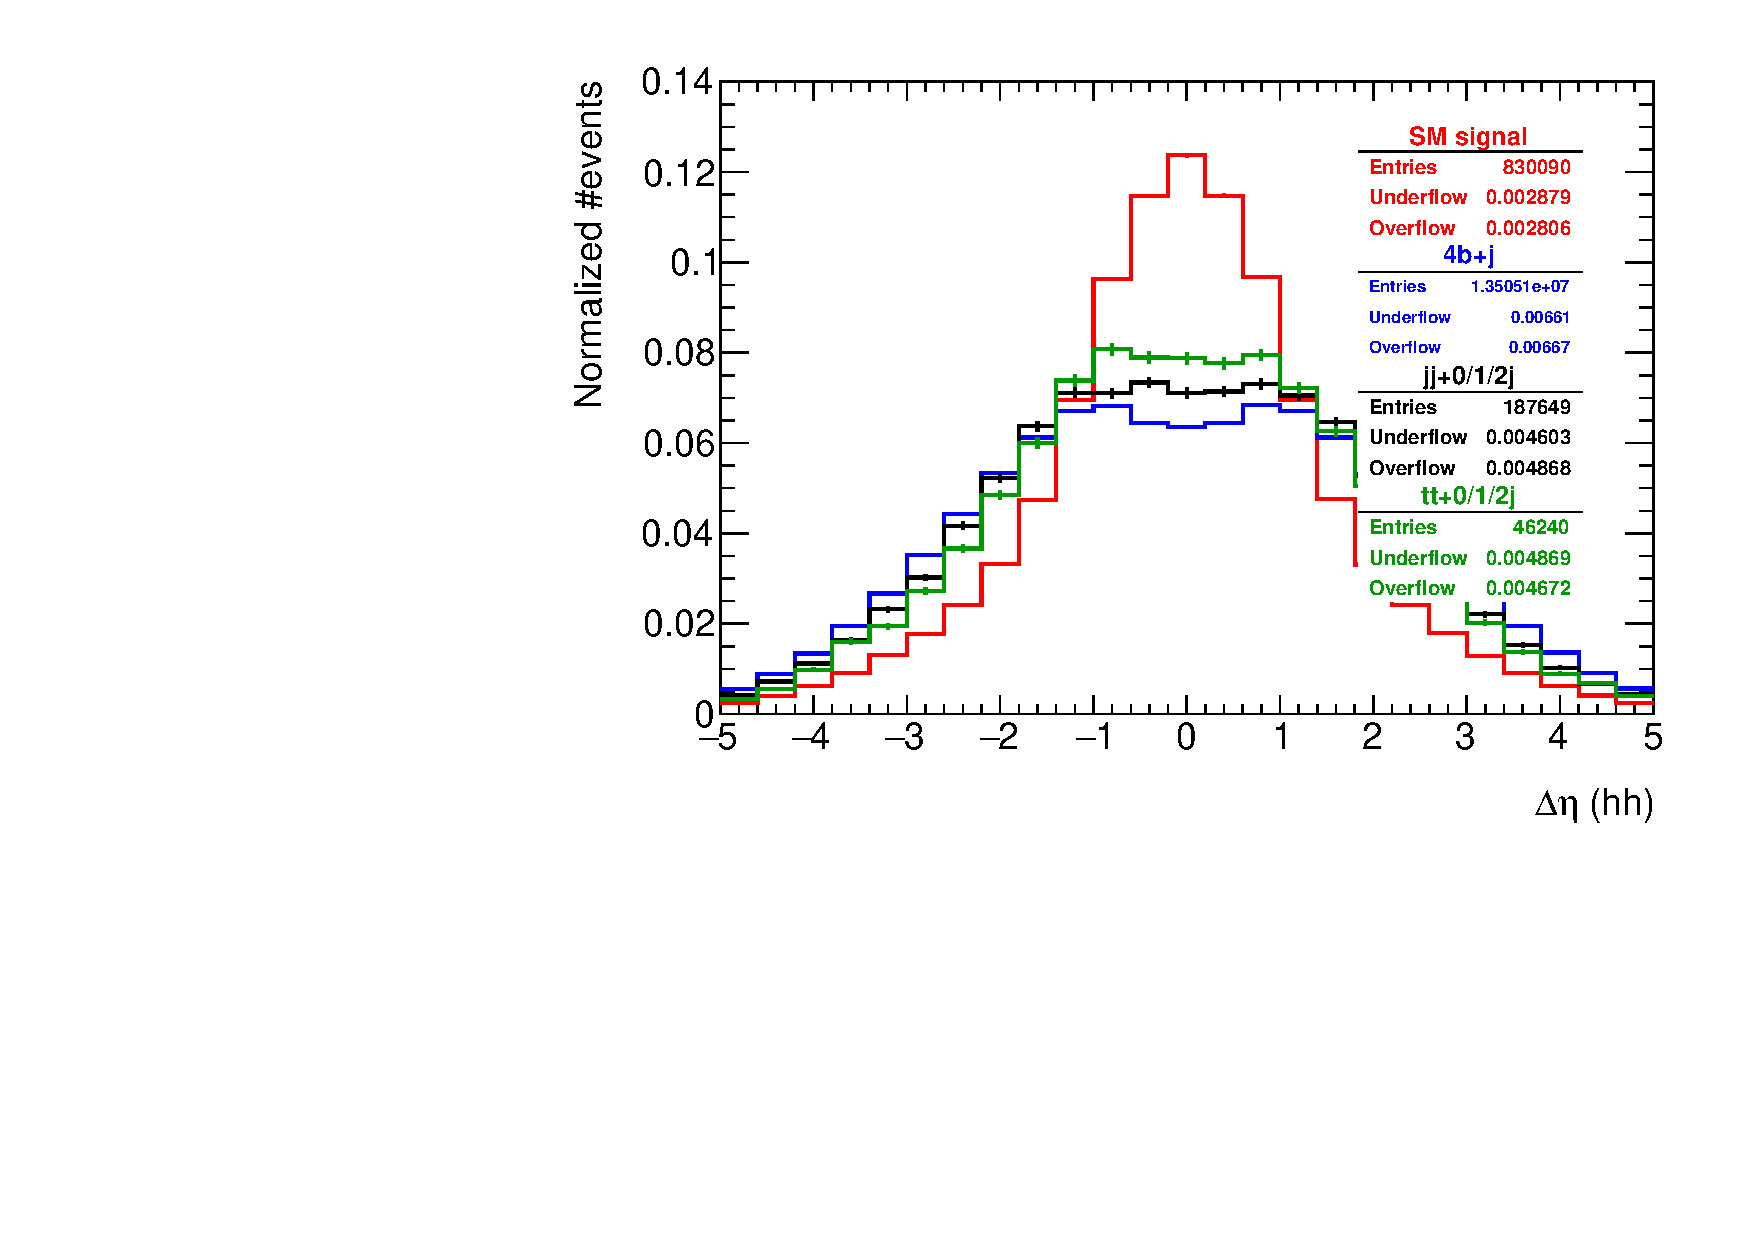
\includegraphics[trim={.65cm 0 0 0},clip,width=\linewidth]{./Figures/hist_hh_deltaEta.pdf}
		%\caption{oi}
		%\label{fig:h1_pt}
	\end{minipage}%
	\begin{minipage}{.5\textwidth}
		\centering
		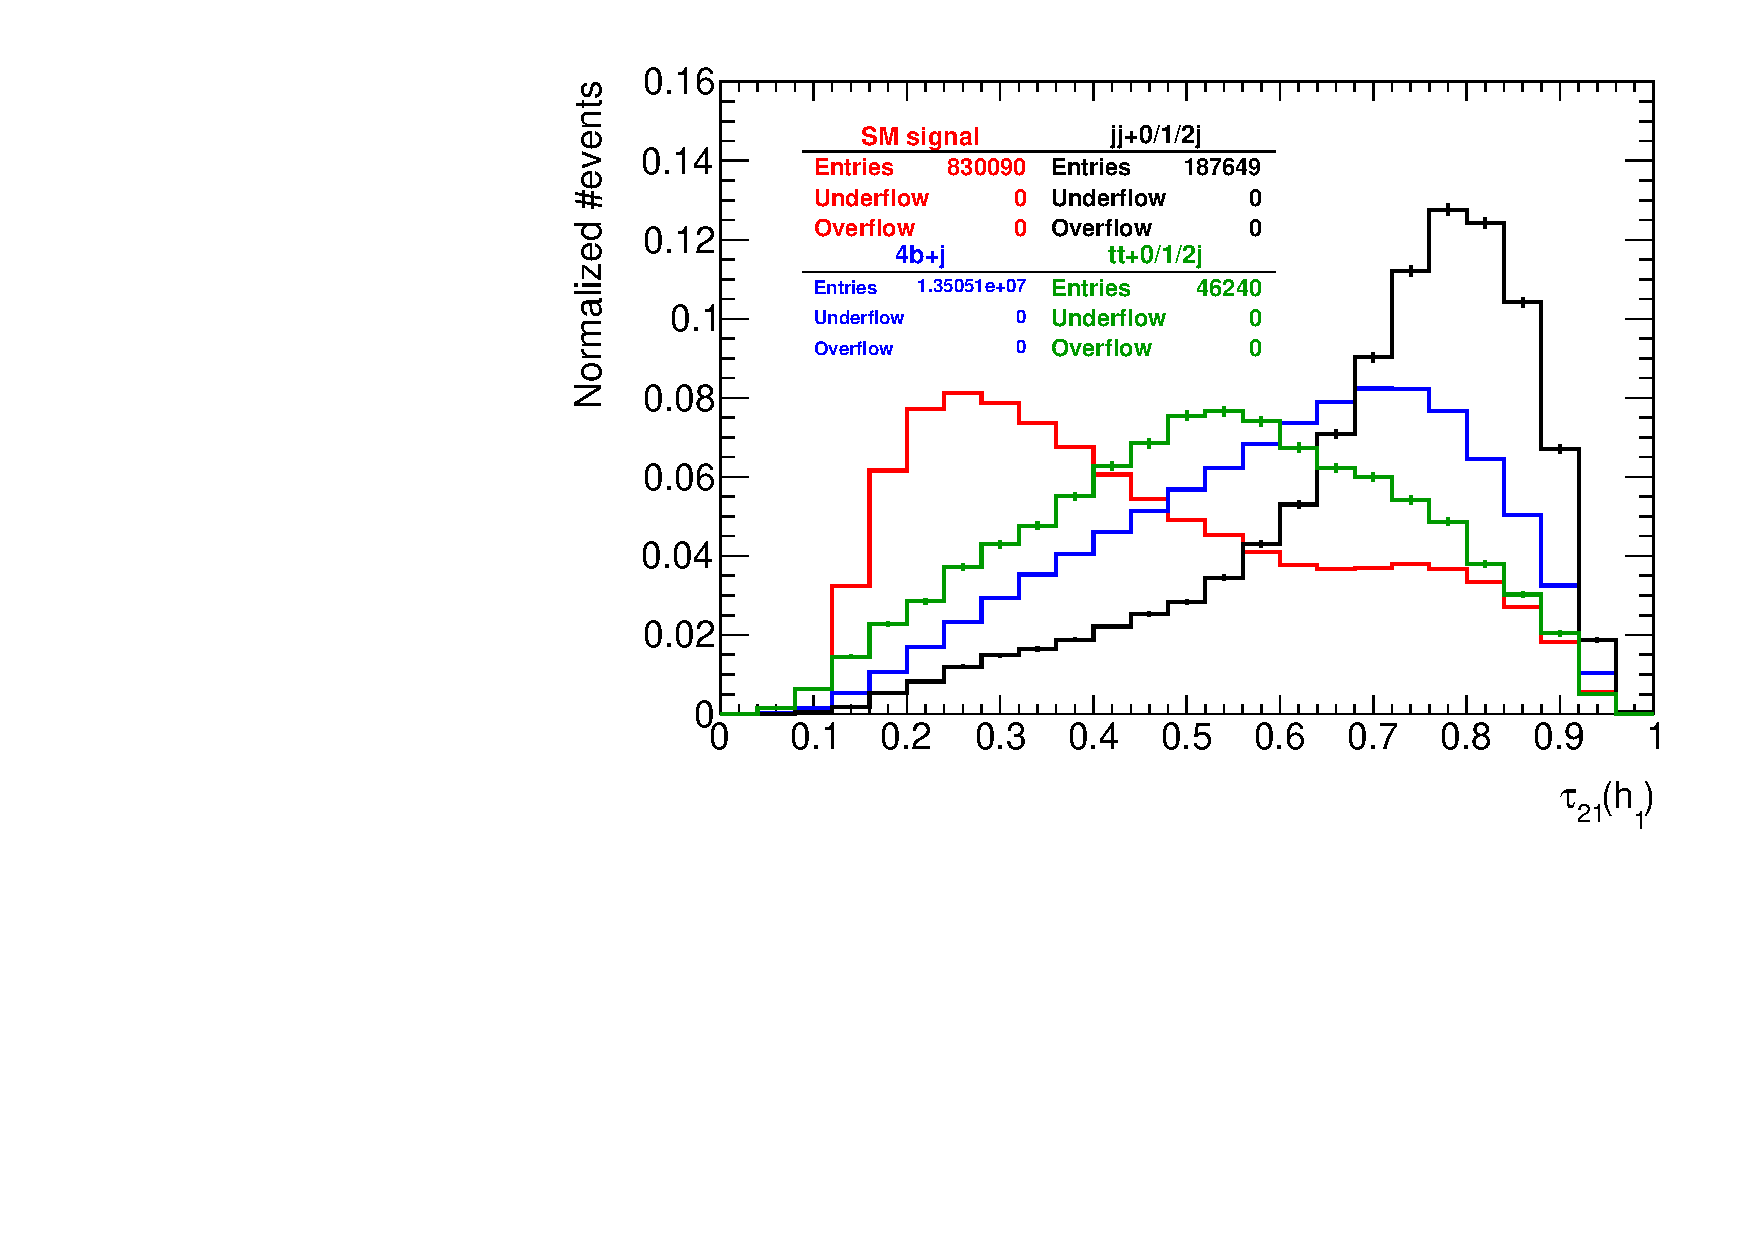
\includegraphics[trim={0 0 .65cm 0},clip,width=\linewidth]{./Figures/hist_h1_tau21.pdf}
			%\caption{oi}
			%\label{fig:h2_pt}
	\end{minipage}
	\begin{minipage}[t]{0.5\textwidth}
		\caption*{(a)}
			%\label{fig1}
	\end{minipage}%%%
	\hfill
	\begin{minipage}[t]{0.5\textwidth}
		\caption*{(b)}
			%\label{fig2}
	\end{minipage}
	\caption{Distributions of the $\Delta\eta$ between the Higgs candidates (a) and of the $\tau_{21}$ variable for the leading Higgs candidate (b).  The histograms are normalized to unit area and include all events that pass the pre-selection cuts.}
	\label{fig:hh_deltaEta_h1_tau21}
\end{figure}
	

\section{Analysis strategy}
\label{section:regions}


%In this analysis we explore three regions: boosted, intermediate and resolved. The details about each region, namely the event topology and selection cuts, are discuss in the following sections (\ref{section:boosted}, \ref{section:intermediate} and \ref{section:resolved}). The regions are orthogonal, i.e, independent. For each event we check if it falls in the boosted category. If it does not we check if it falls in the intermediate category and if it does not we check if it falls in the resolved category. This way, an event falling in the boosted category cannot fall in the intermediate or resolved categories and the same applies for all categories. 
%
%The advantage of performing an analysis in orthogonal regions is that we can then combine the results obtained in each one. For example, we can quadratically add the significances in order to obtained an overall significance. This would not be possible if there were any overlap between the regions. In addition, we have access to increased statistics because we are exploring three different signal topologies. Nonetheless, the selection criteria for each category, as well as the variables to explore, are different and need to be optimized independently.

%- Event topology: two boosted jets each corresponding to a Higgs \\
%- Physics objects: partile flow anti-kT R=0.8 jets (discussion about jet radius in appendix) \\
%- Selection criteria\\
%- Substructure variables \\
%- Optimization (efficiency plots, correlations, MVA...)\\


%\begin{figure}
%	\centering
%	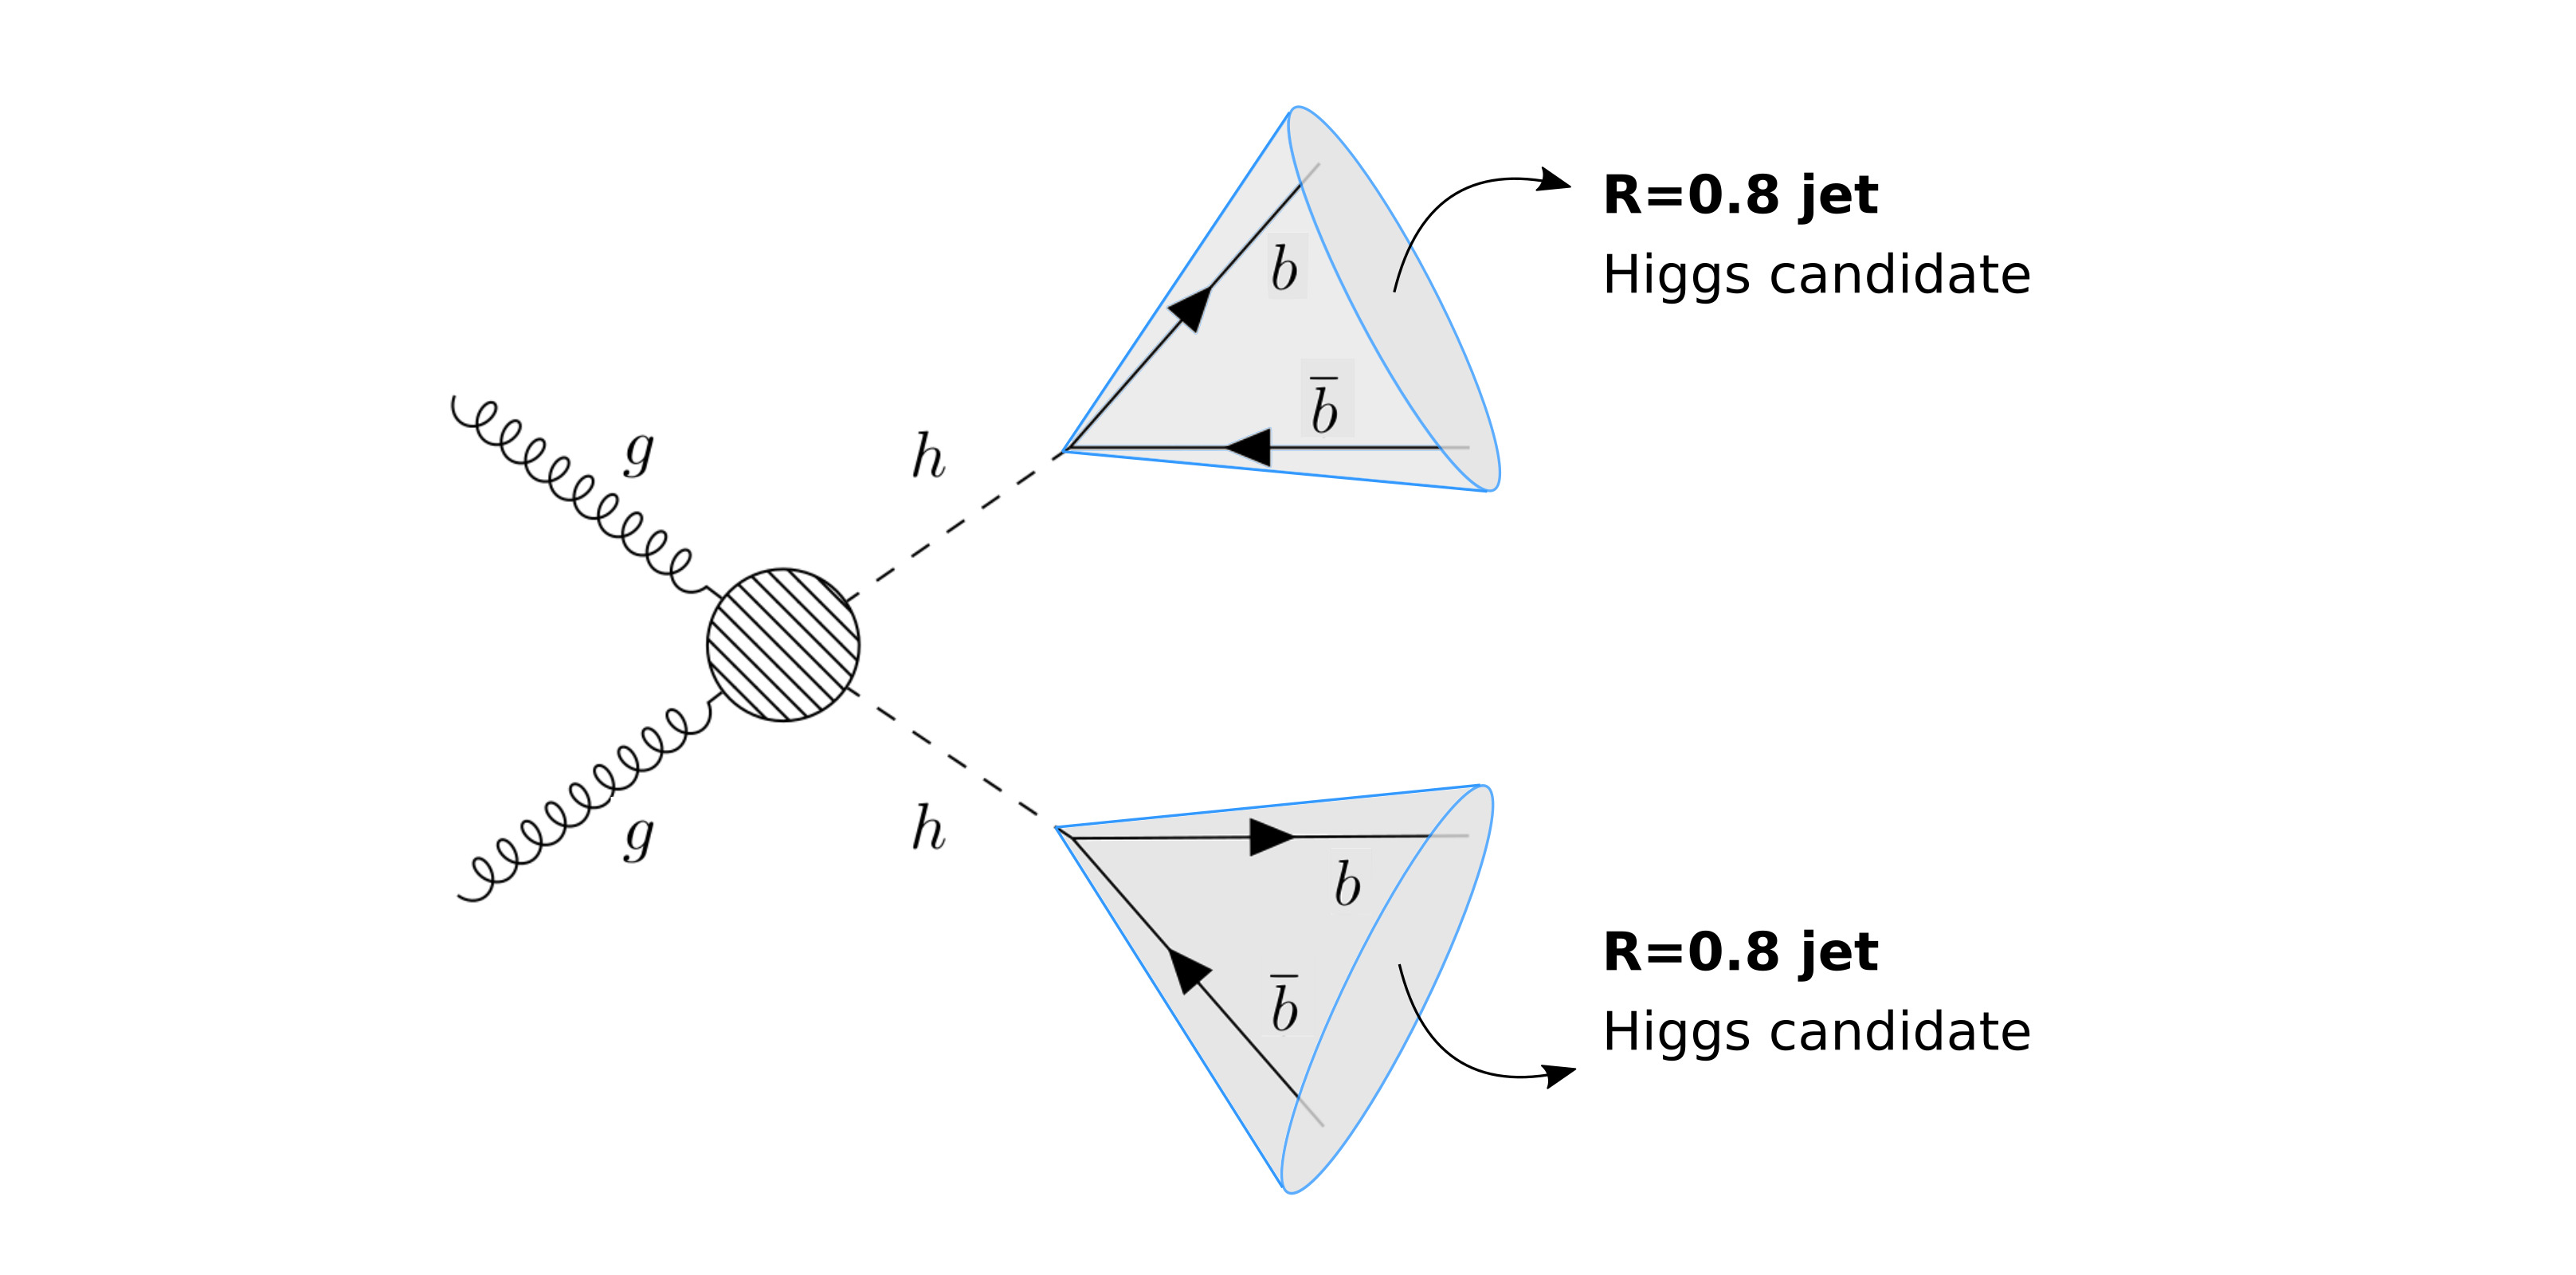
\includegraphics[width=\textwidth]{./Figures/boosted1.png}
%	%\hfill
%	%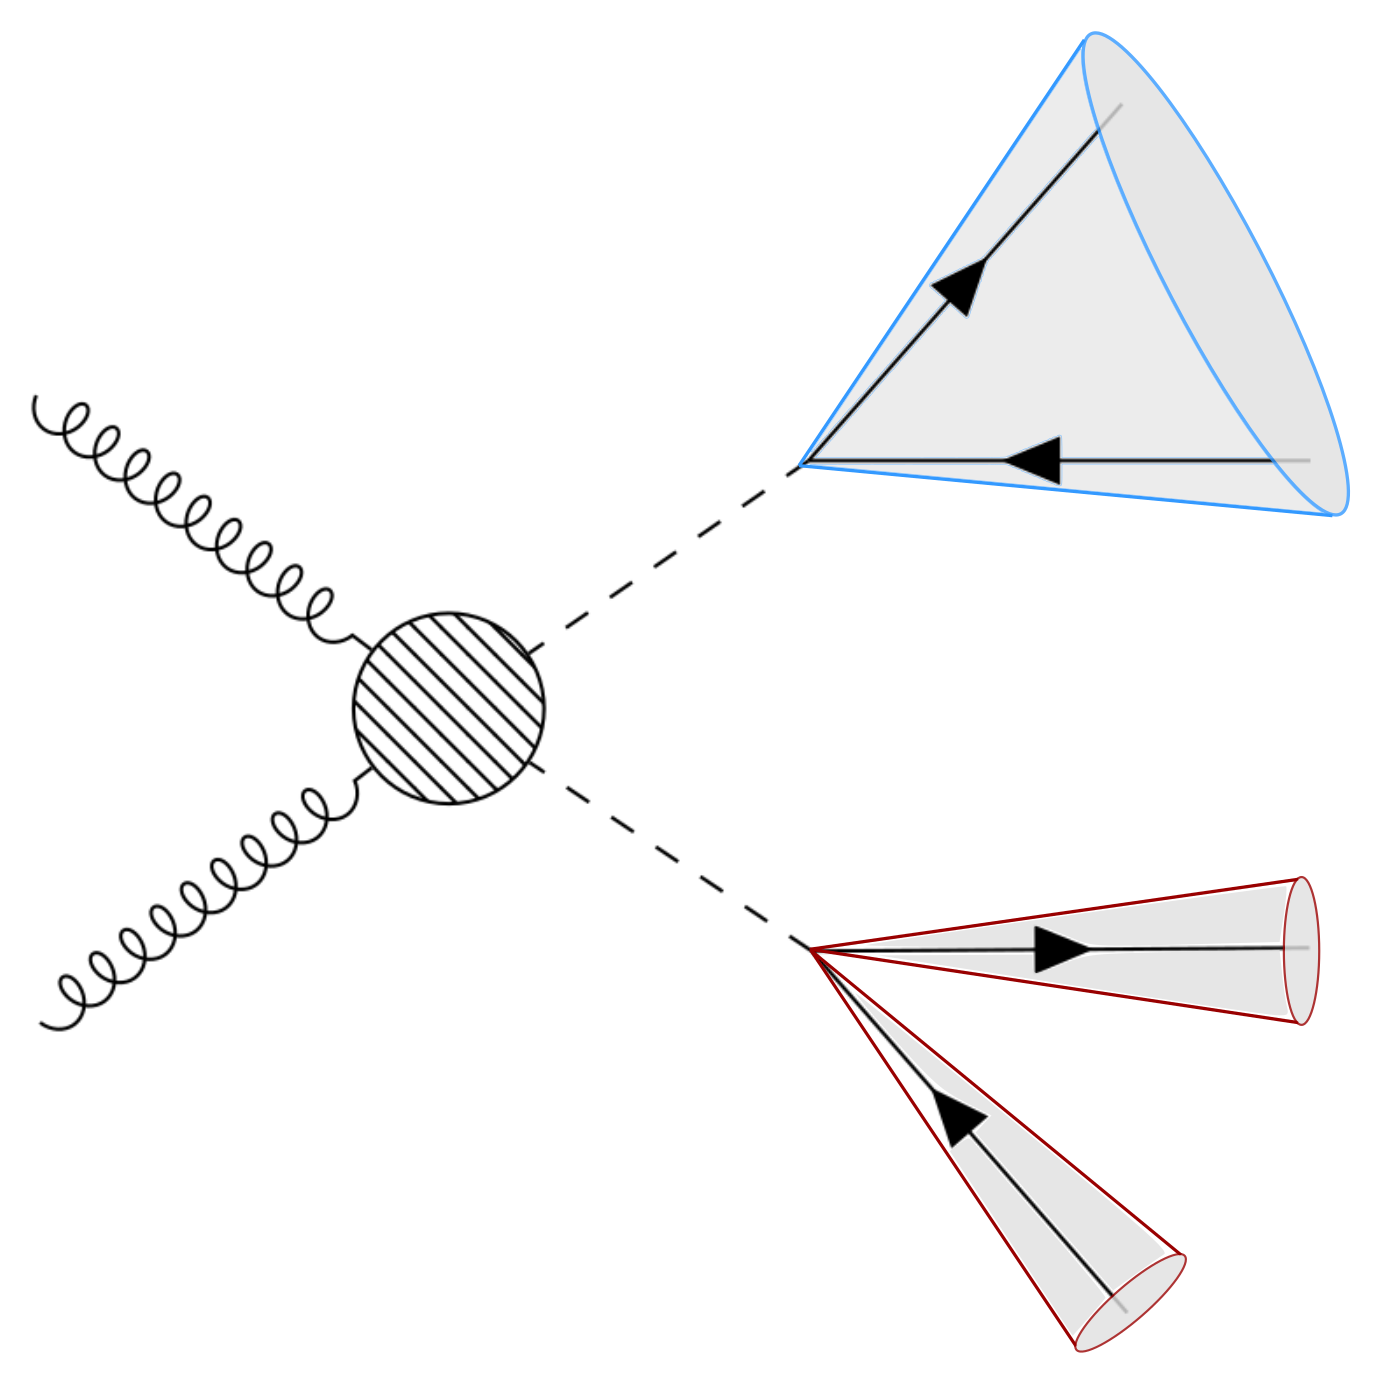
\includegraphics[width=.45\textwidth]{./Figures/inter.png}
%	\caption{Event topology targeted by the boosted analysis region. The blob represents the interaction between the gluons and the Higg bosons that is represented by the Feynman diagrams shown in figure \ref{fig:higgs_pair}.}
%	\label{fig:final_state}
%\end{figure} 

%In this analysis is focused on the bosoted regime. It targets events in which the Higgs bosons have a high Lorentz boost which leads to the collimation of the pairs of b quarks resulting from their decay. As a result, the b quarks cannot be reconstructed in four separated jets. Therefore, two pairs of b quarks are reconstructed using two jets with a larger R parameter. Each jet is expected to contain the b quarks coming from one of the Higgs bosons and works as a proxy for the properties of that Higgs boson.

As already discussed, this analysis targets events in which at least two large-$R$ jets are reconstructed. The jet with the highest momentum is assumed to correspond to the leading Higgs candidate and the jet with the second highest momentum to the sub-leading one. Both the leading and sub-leading jets must be b-tagged in order for the event to be accepted.

The events are reconstructed using particle flow or pure calorimeter jets with $R=0.8$, clustered with the anti-$k_T$ algorithm. We perform the b-tagging of jets using truth level information. Jets with a large-$R$ parameter cannot be b-tagged using the Delphes default algorithm. The tagging of large R jets is an ambiguous task that can be performed in several different ways. Therefore, we implemented our own b-tagging algorithm that is described in section \ref{sec:btagging}. 

In this section, we present the baseline analysis based on cuts on kinematic and substructure variables. An optimized version of the analysis is also presented and compared to the baseline. The optimization is based on the significance ($S/\sqrt{B}$) as a function of the cut threshold for a given variable. We also describe how statistical and systematic uncertainties are estimated. 

\subsection{Implementation of b-tagging}
\label{sec:btagging}

%\begin{figure}
%	\centering
%	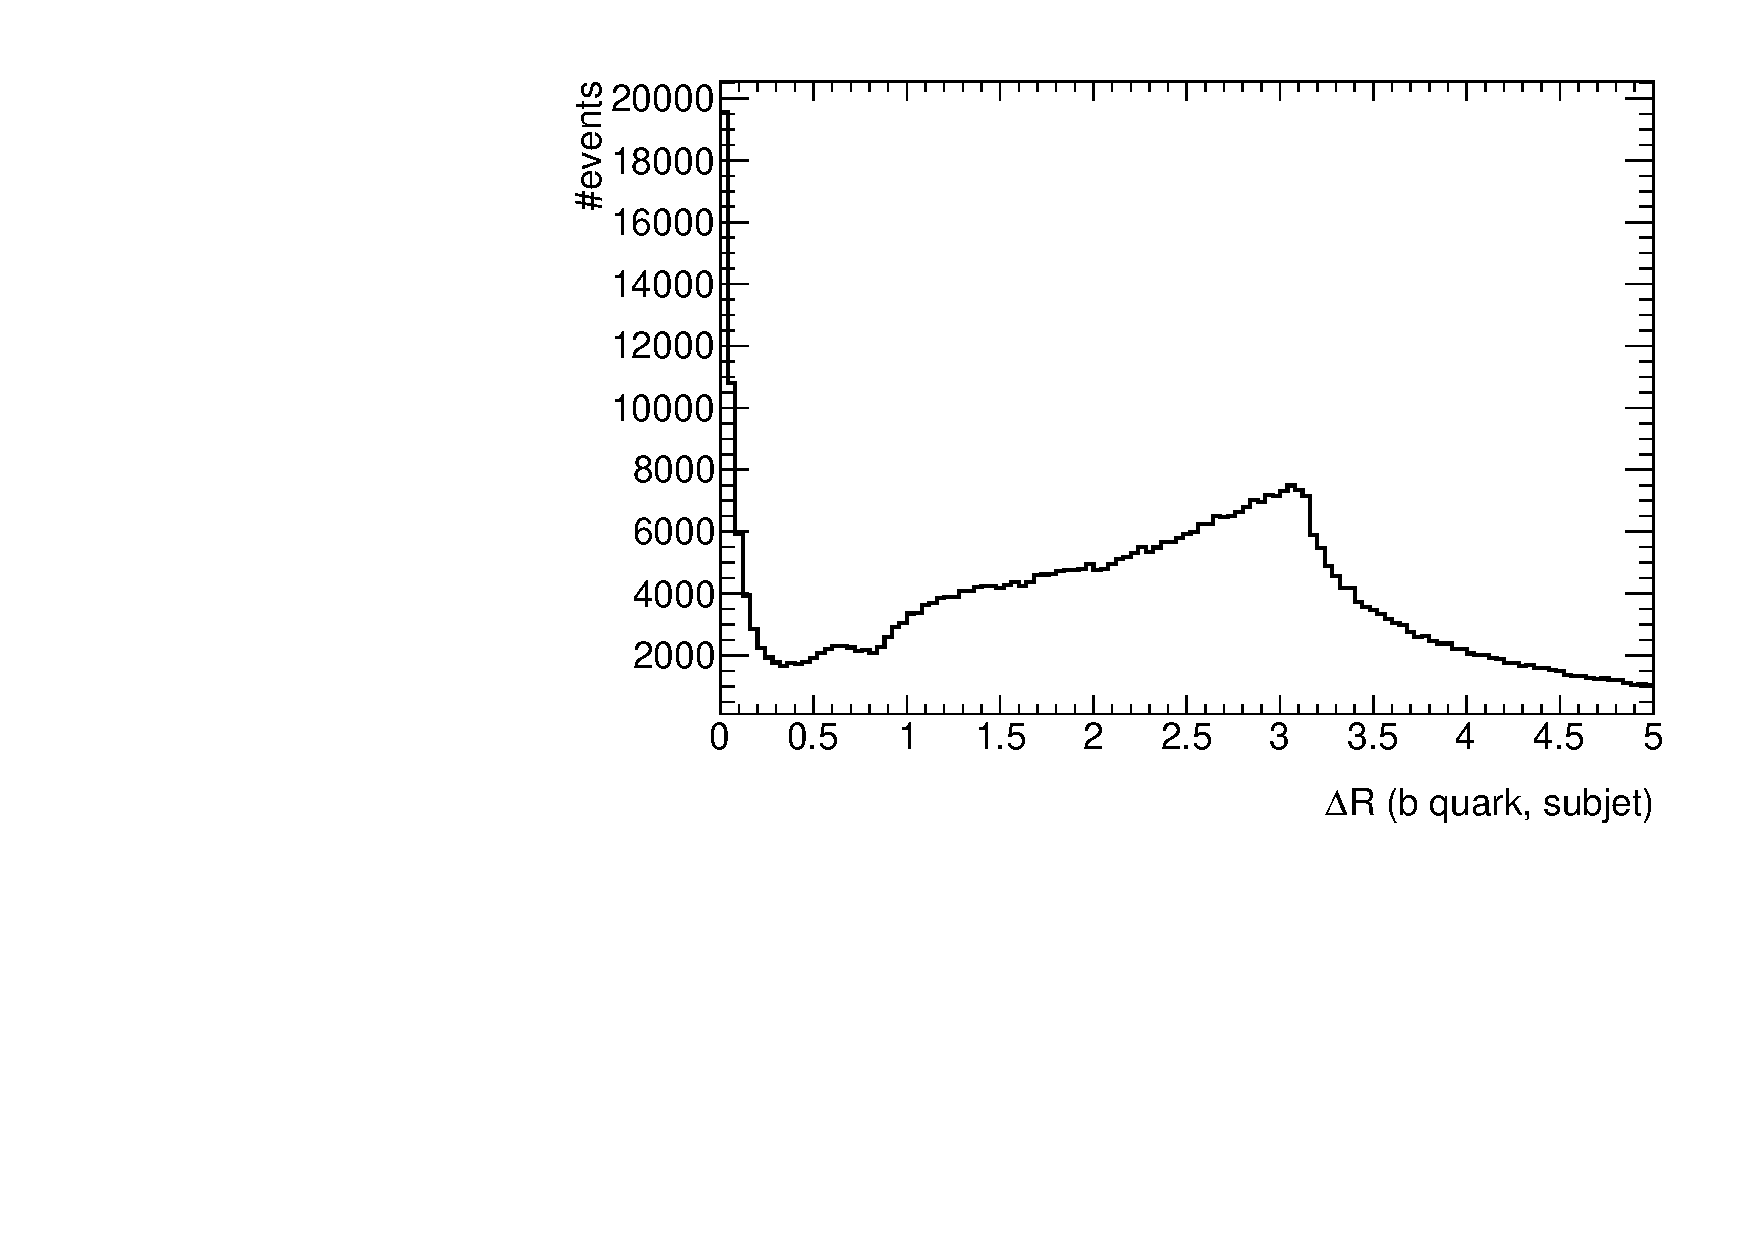
\includegraphics[width=0.5\textwidth]{./Figures/deltaR_bsubjet}
%	\caption{Minimum $\Delta R$ between b quarks and subjets of the $R=0.8$ jets in a $hh\rightarrow b\overline{b}b\overline{b}$ after requiring the existence of at least two large-$R$ jets.} 
%	\label{fig:deltaR_bsubjet}
%\end{figure}

\begin{wrapfigure}{R}{0.45\textwidth}
	\centering
	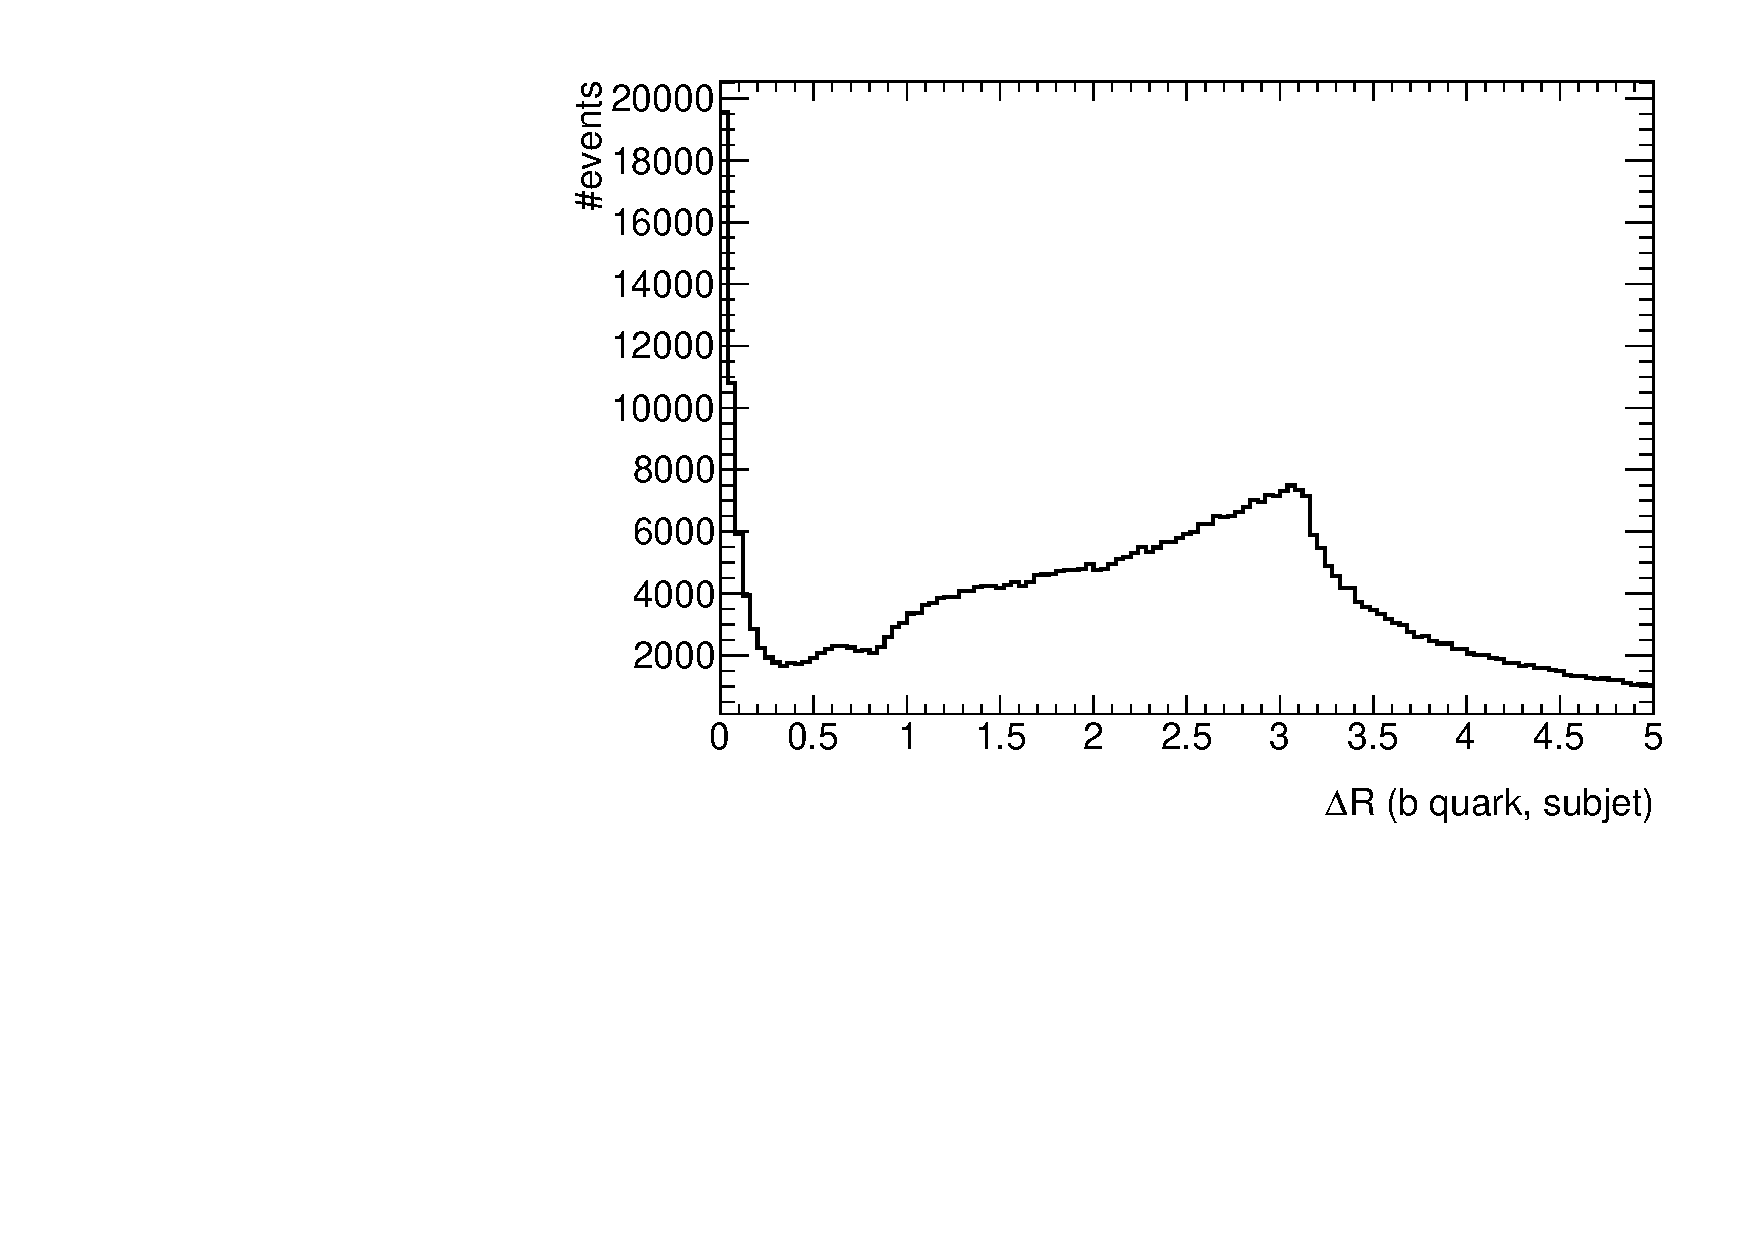
\includegraphics[width=0.45\textwidth]{./Figures/deltaR_bsubjet}
	\caption{\label{fig:deltaR_bsubjet}Minimum $\Delta R$ between b quarks and subjets of the $R=0.8$ jets in a $hh\rightarrow b\overline{b}b\overline{b}$ after requiring the existence of at least two large-$R$ jets.}
\end{wrapfigure}

For each jet, the two hardest subjets are found using the mass drop procedure. It might happen that there are not two subjets because the algorithm's criteria are not met. In that case, the jet is rejected. For each event, we compute the $\Delta R$ distance between all b and c quarks with Pythia status equal to $23$ \cite{Pythia6manual} and with $p_T>10$ GeV and each subjet ($\Delta R(\text{subjet,parton})$). Particles with status $23$ result directly from the hardest subprocess. We consider that a subjet is matched to a given quark if $\Delta R(\text{subjet,parton})<0.3$, based on figure \ref{fig:deltaR_bsubjet}. If the subjet is matched to at least one b quark, we b-tag the subjet with a given probability. If the subjet is not matched to any b quark but it is matched to at least one c quark we apply a c mistag rate. If the subjet is not matched to any b or c quark we apply a light-jet mistag rate. This allows for a more realistic modeling of the imperfect b-tagging performance, where light quark or c quark initiated jets may fake b jets. The b-tag probability and mistag rates were obtained from the Delphes FCC-hh card. They depend on the momentum of the jet and on its $\eta$ coordinate. They are summarized in table \ref{table:btag}. The b-tagging probabilities are given in black and the c and light mis tagging probabilities are given in blue and red, respectively. Note that a jet cannot be b-tagged if $|\eta|>4$ or if its momentum is smaller than $10$ GeV or larger than $15000$ GeV.

In terms of the technical implementation, the b-tagging algorithm works as follows: for each subjet we look for a truth-level b quark within $\Delta R=0.3$ of the subjet and calculate the b-tagging and mistagging efficiencies using the expressions in table \ref{table:btag}, where $p_T$ and $\eta$ refer to the subjet. If a b quark is found we generate a random number between $0$ and $1$. If this number is smaller than the b-tagging efficiency, we consider the subjet to be b-tagged. If the subjet is not b-tagged we look for truth-level c quarks within $\Delta R=0.3$ of the subjet. If one is found we generate a new random number between $0$ and $1$ and if the number is smaller than the c mistag probability we consider the subjet to be b-tagged. If the subjet is still not b-tagged we generate a random number between $0$ and $1$ and consider the subjet b-tagged if the number is smaller than the light-jet mistag probability. 

\begin{table}
	\centering
	\caption{b-Tagging (black), c (blue) and light (red) mistag probabilities as a function of $\eta$ and $p_T$ of the (sub)jet. The momentum dependent factor, $\left(1-p_T/15000\right)$, is common to the three probabilities.}
	\begin{tabular}{llll}
		\toprule 
		\backslashbox{$\eta$}{$p_T$} & $10<p_T<500$ & $500<p_T<15000$ &  \\
		\midrule
		$|\eta|<2.5$ & $0.85;\textcolor{blue}{0.05};\textcolor{red}{0.01} $ & $(0.85;\textcolor{blue}{0.05};\textcolor{red}{0.01})\times\left(1-p_T/15000\right)$ &   \\
		\rowcolor{black!7} $2.5<|\eta|<4.0$ & $0.64;\textcolor{blue}{0.03};\textcolor{red}{0.0075}$ & $(0.64;\textcolor{blue}{0.03};\textcolor{red}{0.0075})\times\left(1-p_T/15000\right)$ &  \\
		\bottomrule
	\end{tabular}
	\label{table:btag}
\end{table}

%\subsection{Event pre-selection}
%
%TO INCLUDE: \\
%- discussion on trigger requirements: important in real analysis\\
%- show and discuss some distributions: invariant mass (h, hh), momentum, tau21, delta eta (hh), more substructure variables (may be all that we considered relevant)\\
%- compare with other articles/analysis ? \\
%
%--------------------------------------------------------------------------------------------------
%
%We require at least two b-tagged $R=0.8$ jets (which corresponds to at least four b-tagged subjets, at least two in each $R=0.8$ jet). In addition, the leading and sub leading jets must have $p_T\geq200$ GeV in order for the event to be accepted. Due to the b-tagging efficiency formulas, there is a natural cutoff at $|\eta|=4$ so we do not place any additional cut in $\eta$. From now on, these cuts are referred to as pre-selection cuts. 

\subsection{Baseline analysis}

The analysis described in this section and in section \ref{sec:opt} were developed using the samples simulated with the default FCC-hh detector implementation. The same event selection was then applied to the samples generated using the different detector configurations. %This allows for a straightforward comparison of the results obtained with the different configurations.

As a first step, we implemented a baseline analysis based on rectangular cuts on kinematic and substructure variables. Firstly, we apply cuts on the transverse momenta of the leading and sub leading Higgs candidates, $p_T(h_1)$ and $p_T(h_2)$, and of the Higgs pair, $p_T(hh)$:
\begin{equation}
	p_T(h_1)>400 ~\text{GeV}, \quad p_T(h_2)>350 ~\text{GeV}, \quad p_T(hh)>100 ~\text{GeV}.
\end{equation}
The effect of these cuts may be appreciated from the distributions shown in figures \ref{fig:pt_stack}(a), \ref{fig:pt_stack}(b) and \ref{fig:sub_stack}(a) and guarantee that we are choosing events for which the Higgs candidates are sufficiently boosted. In addition, a high threshold for the $p_T$ of the jets suppresses $t\overline{t}$ events because the decay products of the top quark are reconstructed as a single jet.

We then apply a cut on the $\tau_{21}$ of the leading Higgs candidate, illustrated in figure \ref{fig:sub_stack}(b), to select jets that are more compatible with a two-prong structure:
\begin{equation}
	\tau_{21}(h_1)<0.55.
\end{equation}
The cut on this variable works as a Higgs tagging method. Therefore we apply the same cut on the $\tau_{21}$ of the sub leading Higgs candidate although that does not necessarily follow from the distribution of $\tau_{21}$ for the sub leading Higgs candidate (which can be found in figure \ref{fig:tau21_h2_stack} in appendix \ref{chapter:extra_plots}).
Then, from the distribution in figure \ref{fig:M_stack}(a), we place a cut on the second Fox-Wolfram momentum (defined in section \ref{section_jet_sub}) of the leading Higgs candidate, $H_2 (h_1)$:
\begin{equation}
	H_2 (h_1)>0.2
\end{equation}
This substructure variable is particularly interesting because it helps supress the $t\overline{t}$ background.

Finally, based on the distribution shown in figure \ref{fig:M_stack}(b), we apply a cut on the softdrop mass of both Higgs candidates, $M_{SD}(h_1,h_2)$. The distribution of $M_{SD}(h_2)$ is similar to this one so we do not show it here. This cut is placed in a window around the nominal SM Higgs mass:
\begin{equation}
	(100\leq M_{SD}(h_1,h_2)\leq 135) ~\text{GeV}.
\end{equation}

Using this analysis, we achieve a significance, $S/\sqrt{B}$, of $5.1\pm0.5~\text{(stat.)}~ ^{+2.5}_{-1.8}~(\text{sys.})$ $\left(1.62\pm 0.16~\text{(stat.)}~^{+0.8}_{-0.6}~\text{(sys.)}\right)$ for an integrated luminosity of $30~(3)~\text{ab}^{-1}$.

\begin{figure}
	\centering
	\begin{minipage}{.5\textwidth}
		\centering
		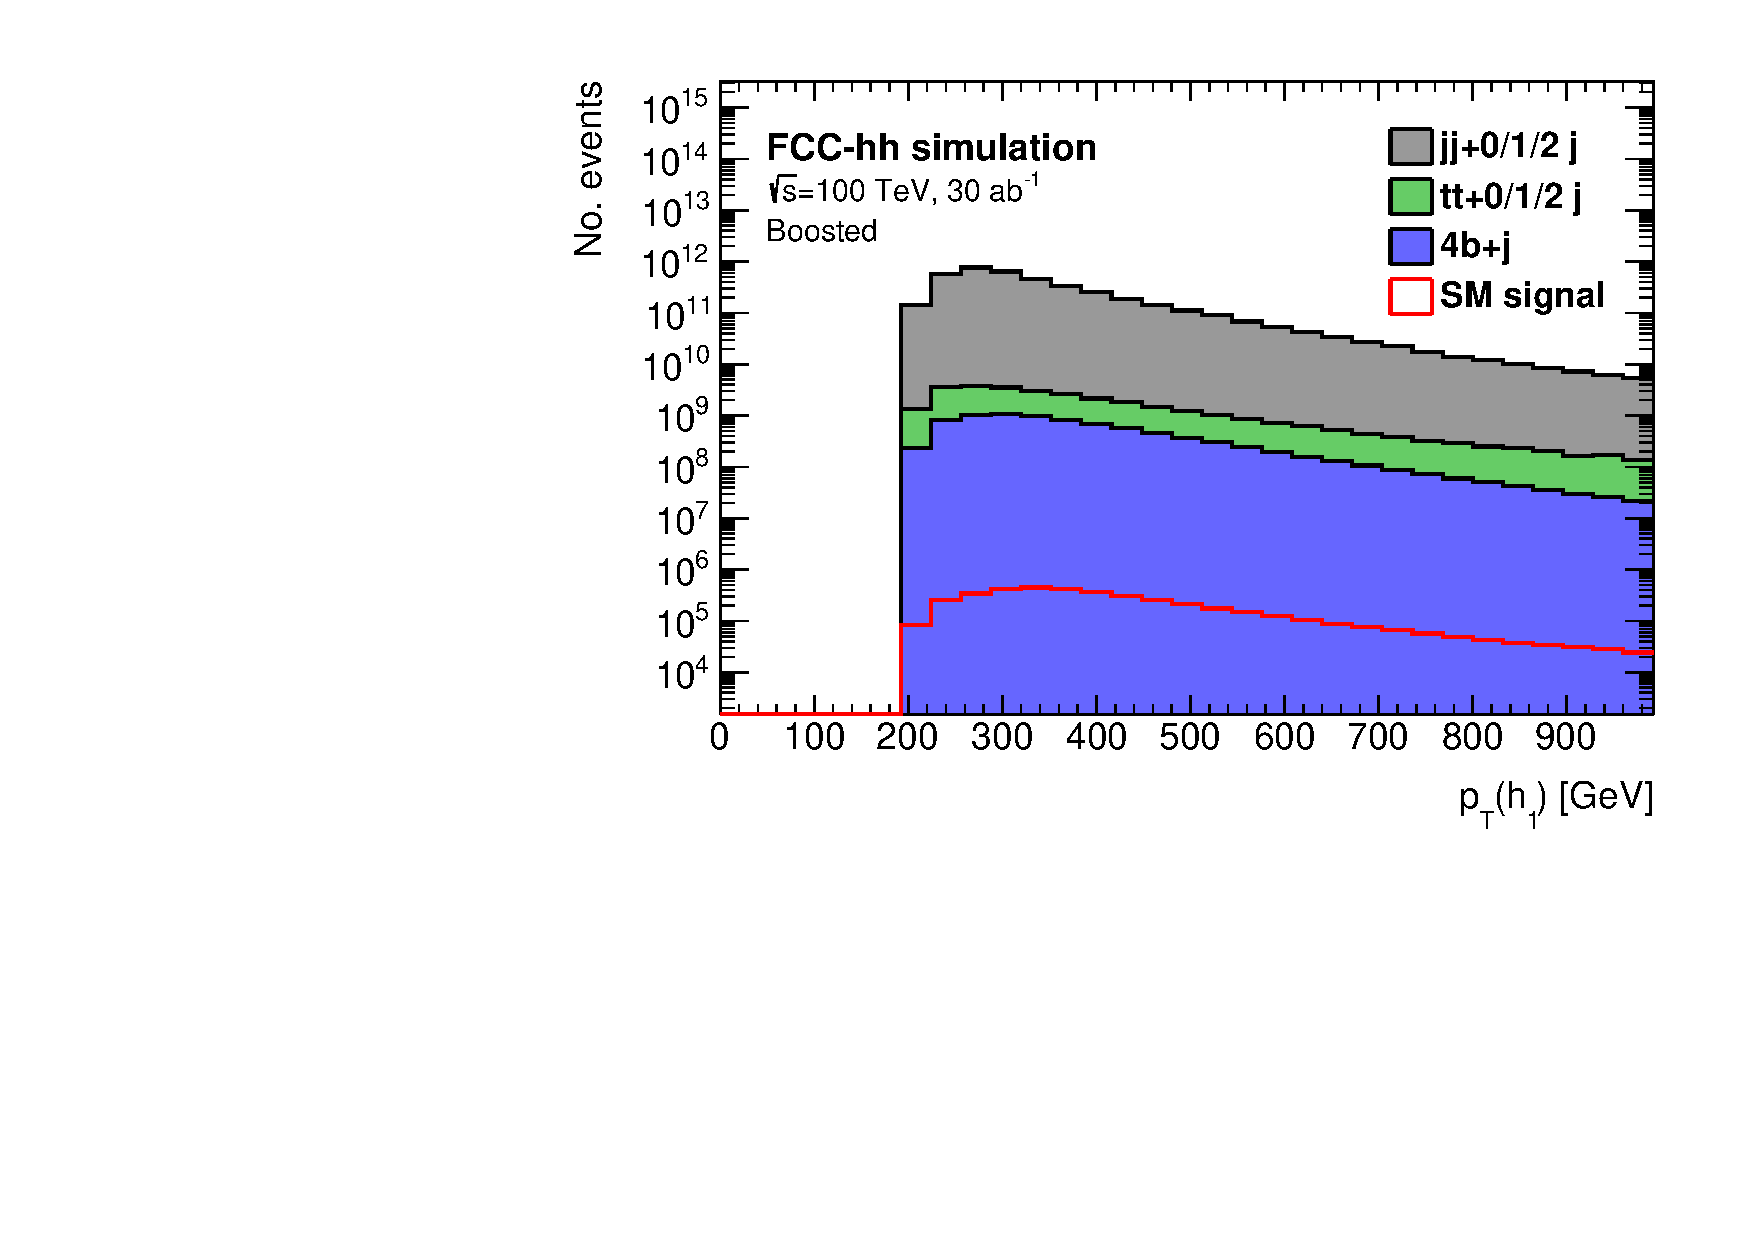
\includegraphics[trim={.65cm 0 0 0},clip,width=\linewidth]{./Figures/hist_h1_pt_stack.pdf}
		%\caption{oi}
		%\label{fig:h1_pt}
	\end{minipage}%
	\begin{minipage}{.5\textwidth}
		\centering
		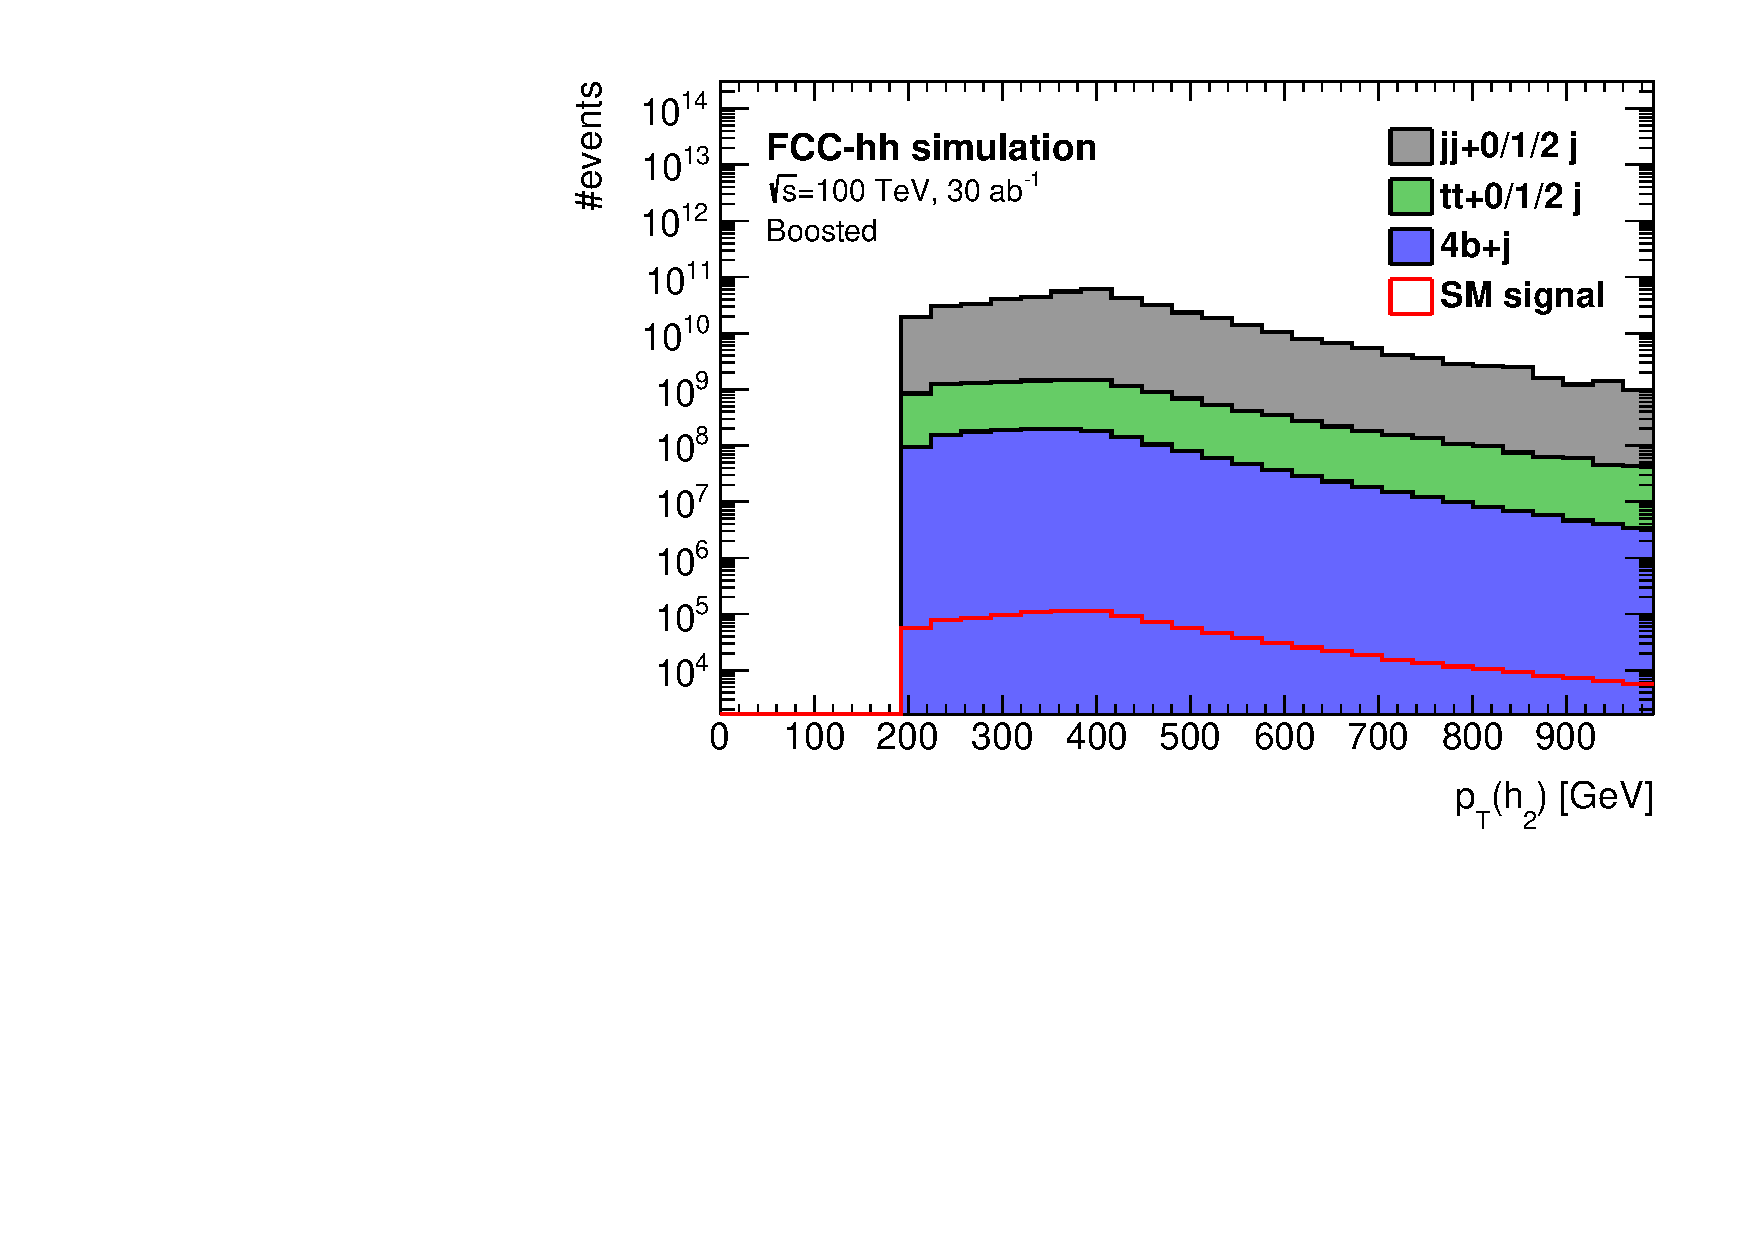
\includegraphics[trim={0 0 .65cm 0},clip,width=\linewidth]{./Figures/hist_h2_pt_stack.pdf}
		%\caption{oi}
		%\label{fig:h2_pt}
	\end{minipage}
	\begin{minipage}[t]{0.5\textwidth}
		\caption*{(a)}
		%\label{fig1}
	\end{minipage}%%%
	\hfill
	\begin{minipage}[t]{0.5\textwidth}
		\caption*{(b)}
		%\label{fig2}
	\end{minipage}
	\caption{$p_T$ distributions for the leading (a) and sub leading Higgs candidates (b). The histograms are normalized to $\mathcal{L}=30~\text{ab}^{-1}$.}
	\label{fig:pt_stack}
\end{figure} 

\begin{figure}
	\centering
	\begin{minipage}{.5\textwidth}
		\centering
		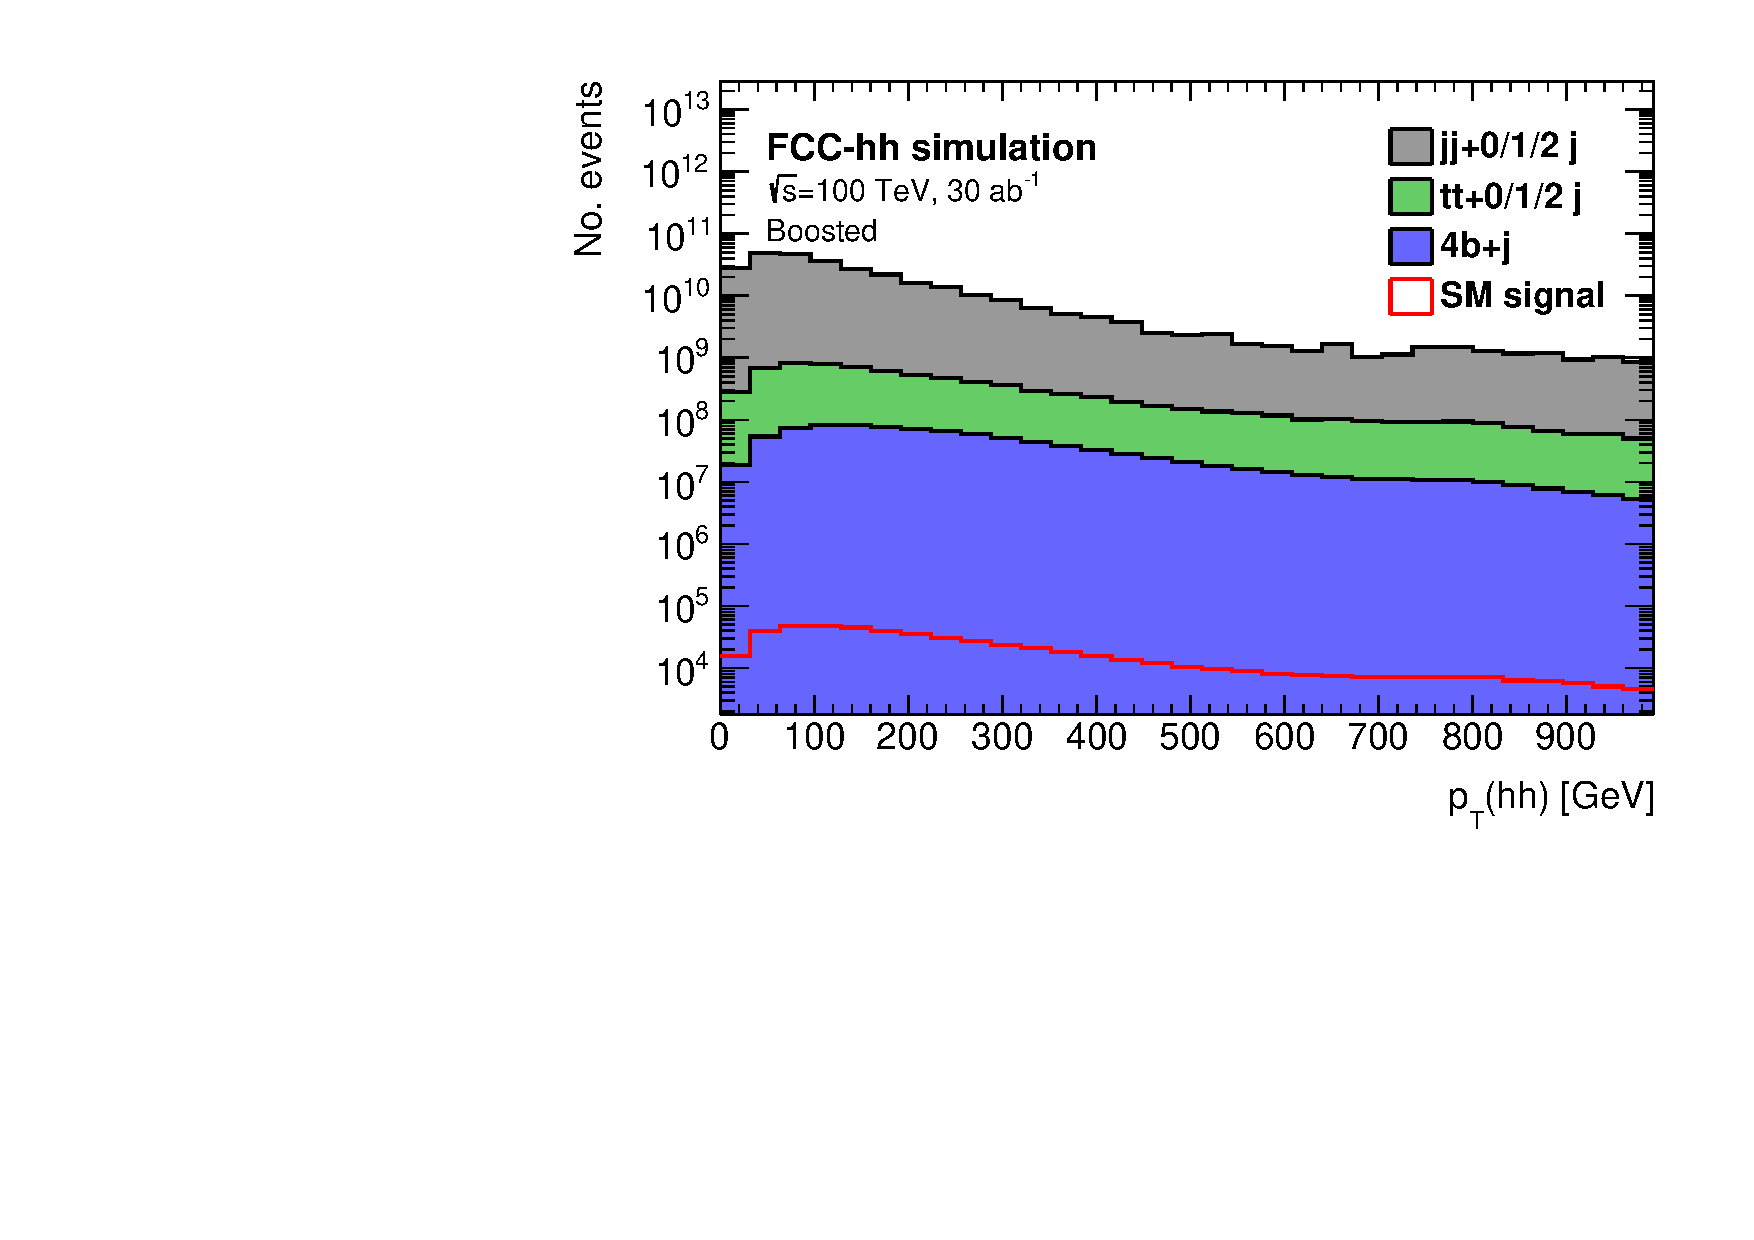
\includegraphics[trim={.65cm 0 0 0},clip,width=\linewidth]{./Figures/hist_hh_pt_stack.pdf}
		%\caption{oi}
		%\label{fig:h1_pt}
	\end{minipage}%
	\begin{minipage}{.5\textwidth}
		\centering
		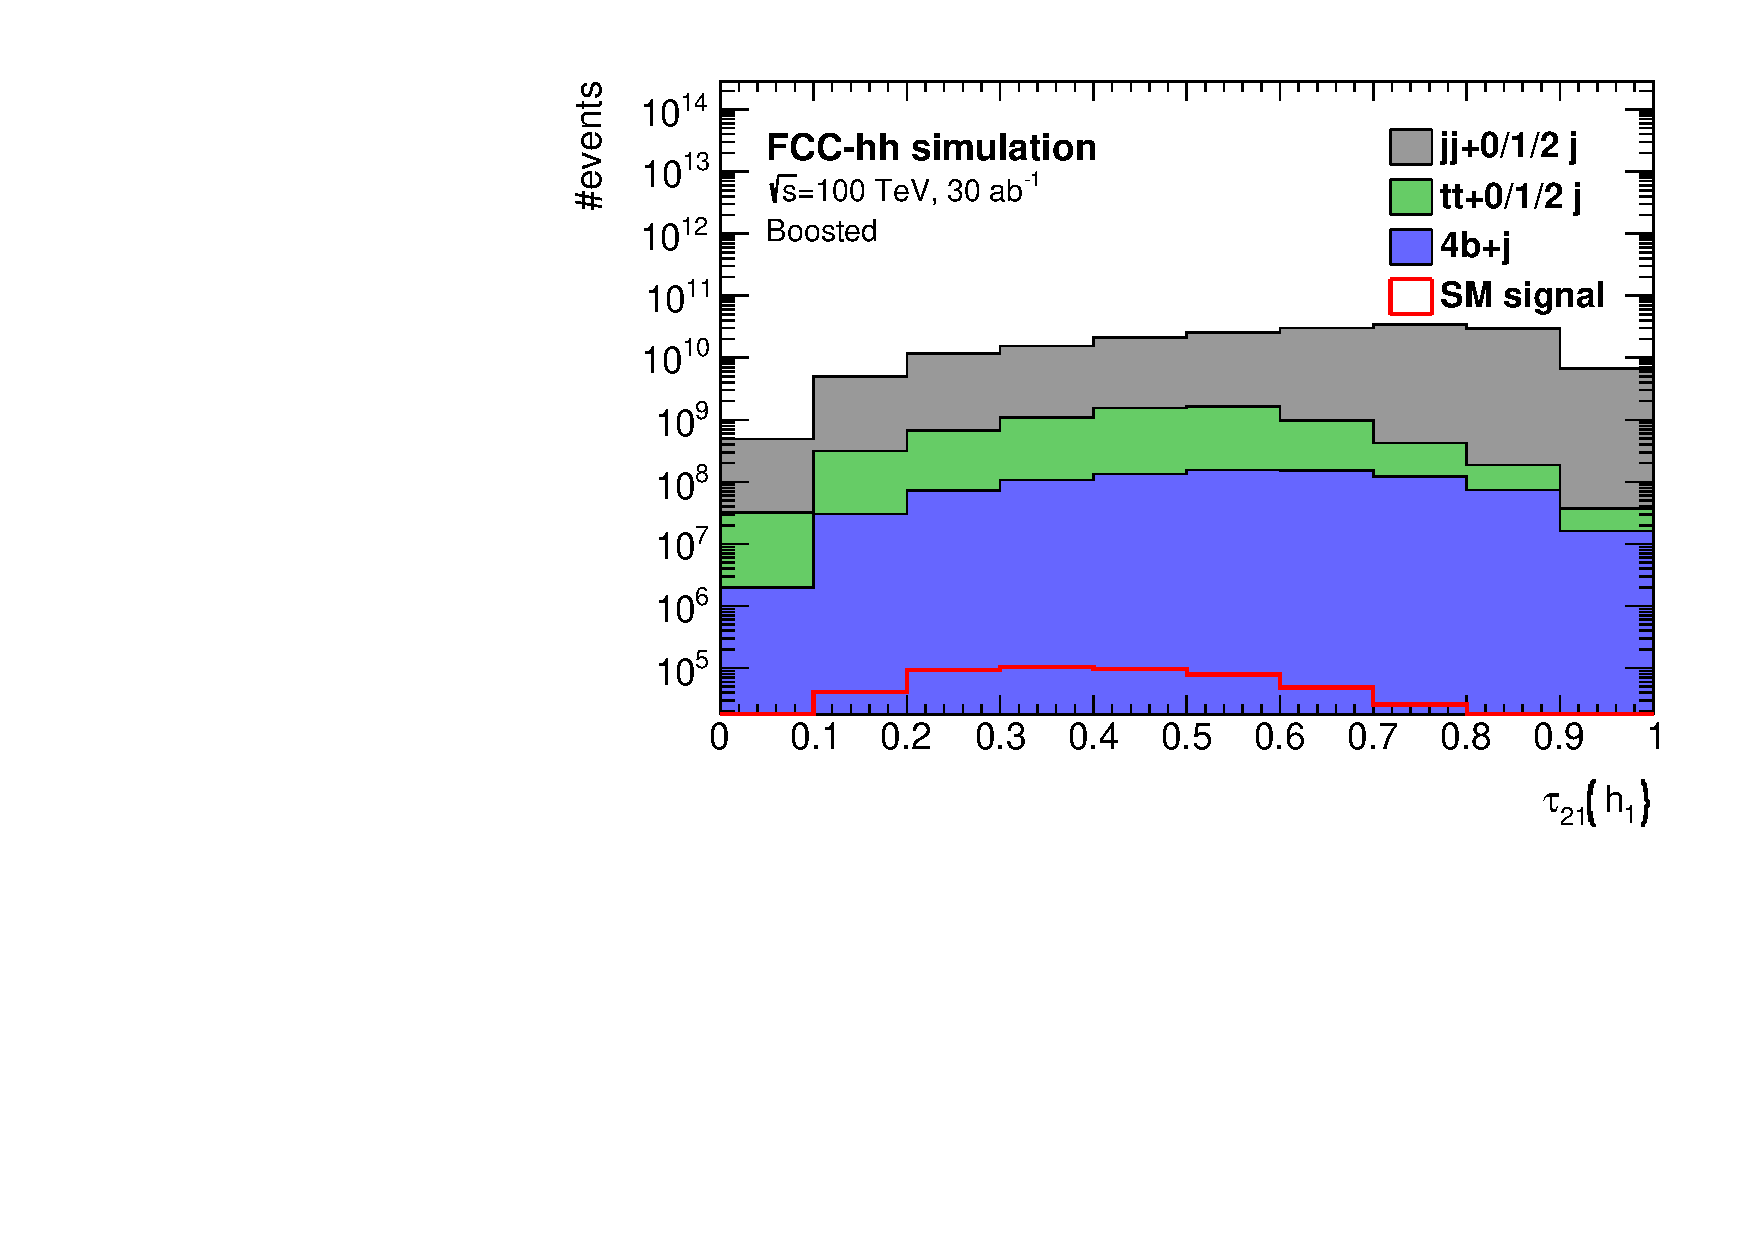
\includegraphics[trim={0 0 .65cm 0},clip,width=\linewidth]{./Figures/hist_h1_tau21_stack.pdf}
		%\caption{oi}
		%\label{fig:h2_pt}
	\end{minipage}
	\begin{minipage}[t]{0.5\textwidth}
		\caption*{(a)}
		%\label{fig1}
	\end{minipage}%%%
	\hfill
	\begin{minipage}[t]{0.5\textwidth}
		\caption*{(b)}
		%\label{fig2}
	\end{minipage}
	\caption{(a) $p_T$ distribution for the Higgs pair, (b) $\tau_{21}$ variable for the leading Higgs candidate. The histograms are normalized to $\mathcal{L}=30~\text{ab}^{-1}$.}
	\label{fig:sub_stack}
\end{figure} 

\begin{figure}
	\centering
	\begin{minipage}{.5\textwidth}
		\centering
		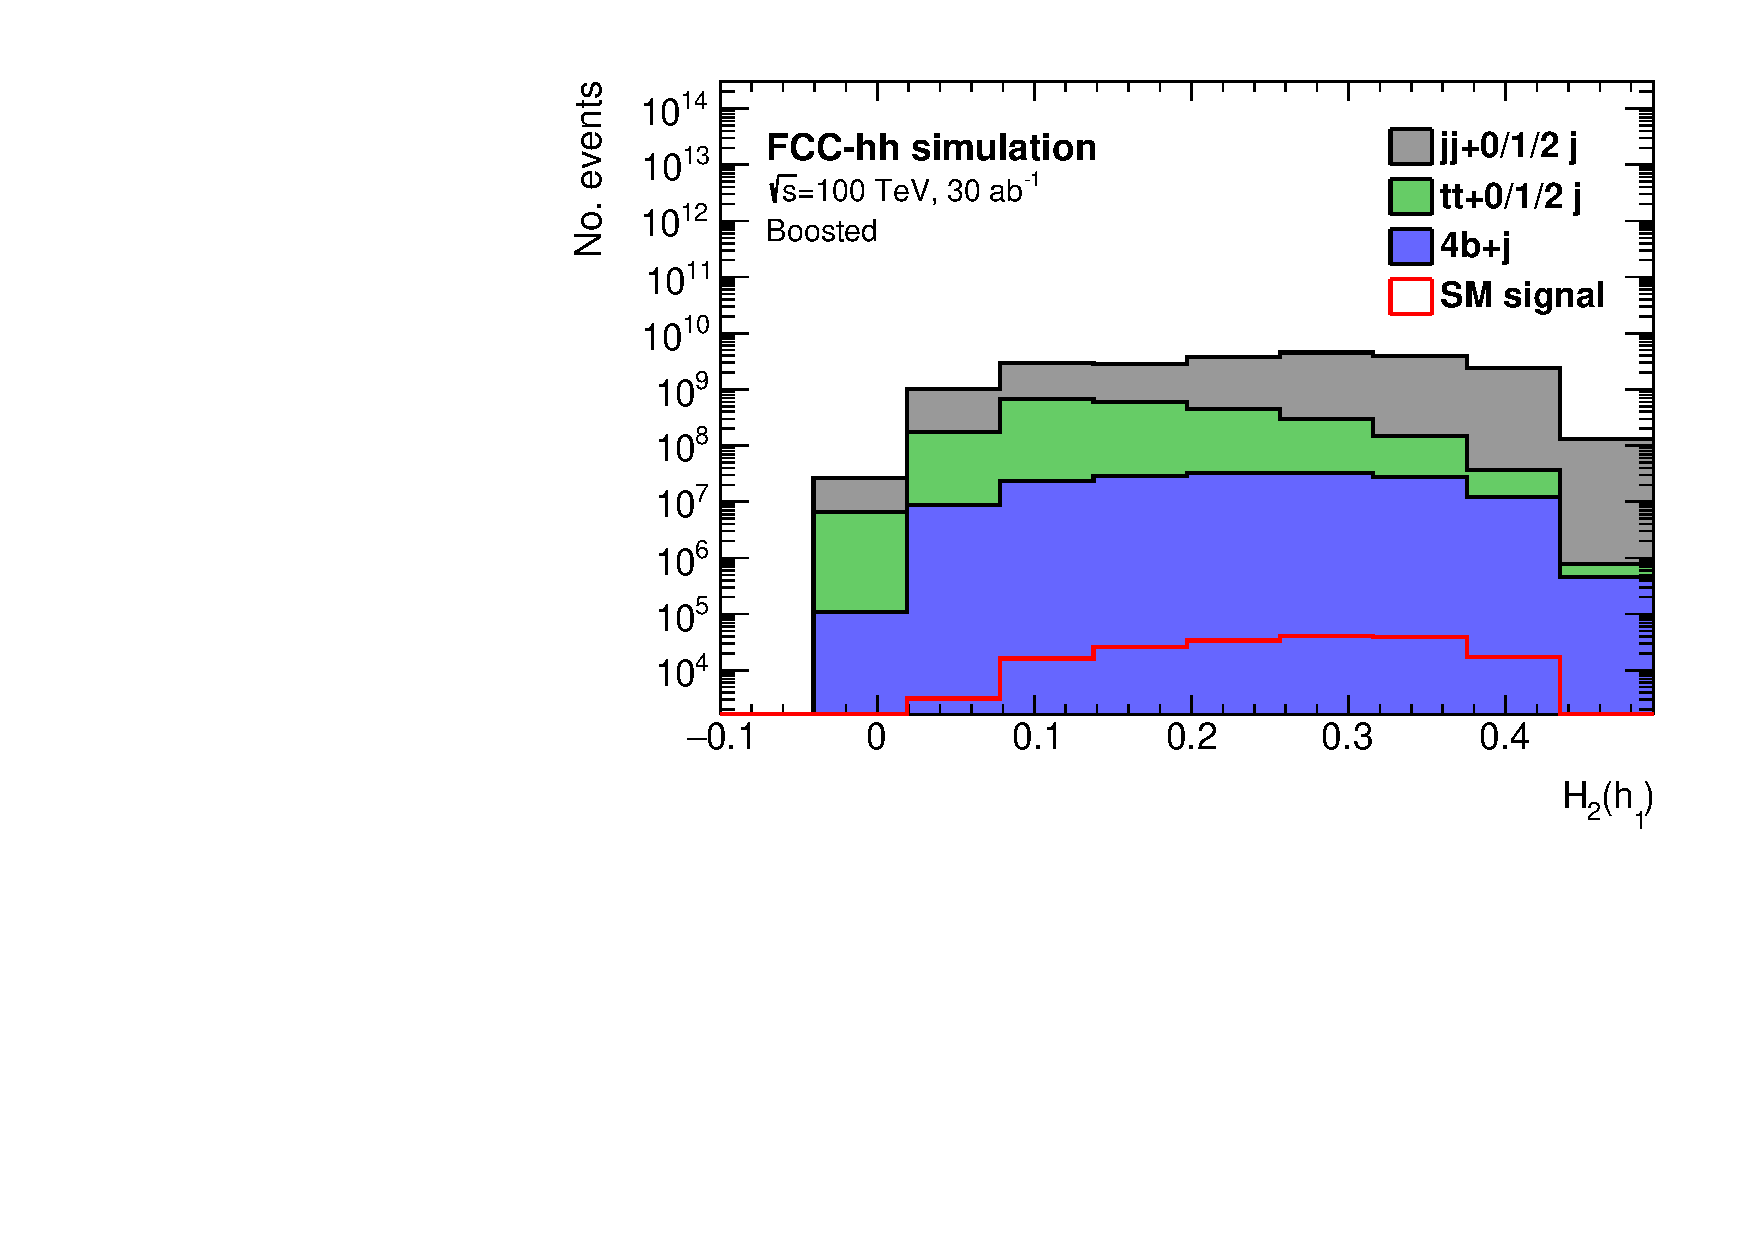
\includegraphics[trim={.65cm 0 0 0},clip,width=\linewidth]{./Figures/hist_h1_FW2_stack.pdf}
		%\caption{oi}
		%\label{fig:h1_pt}
	\end{minipage}%
	\begin{minipage}{.5\textwidth}
		\centering
		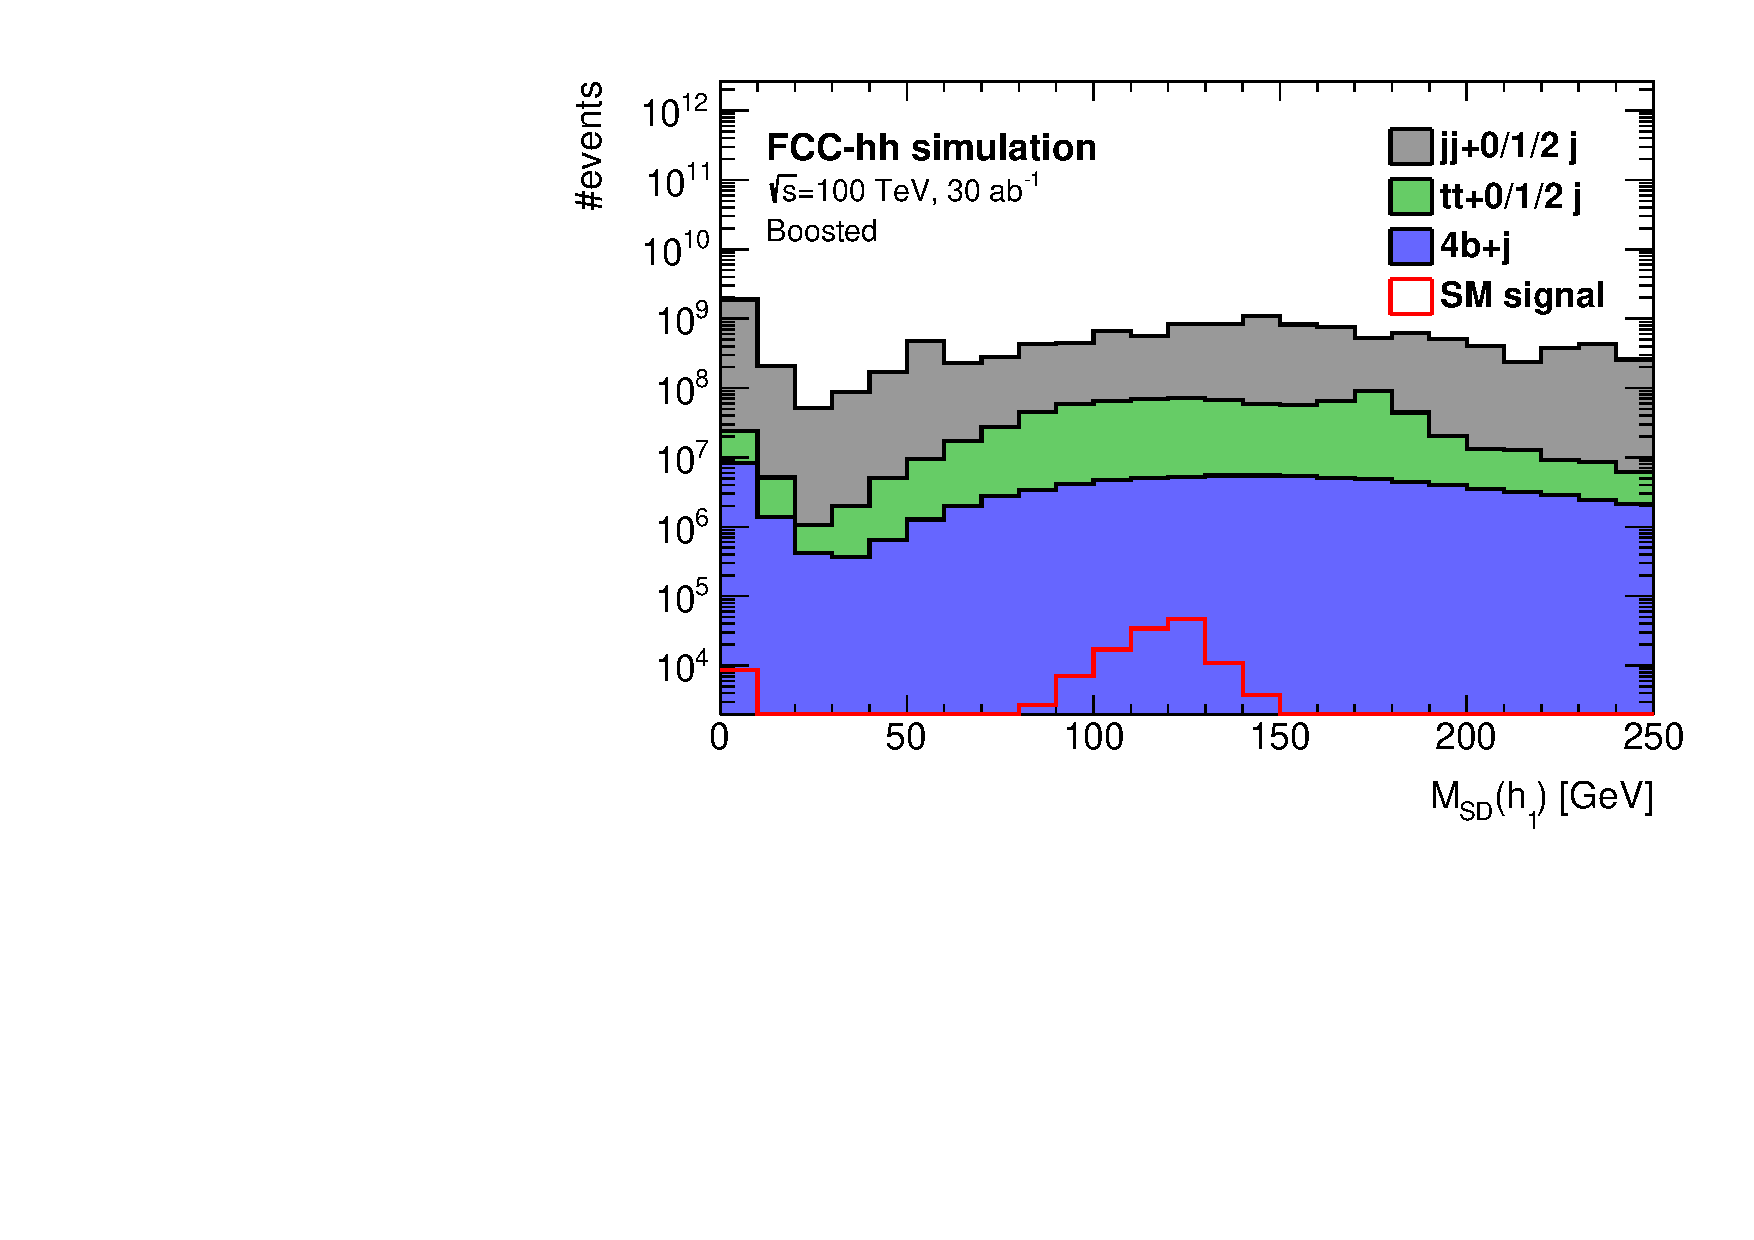
\includegraphics[trim={0 0 .65cm 0},clip,width=\linewidth]{./Figures/hist_h1_softdrop_M_stack.pdf}
		%\caption{oi}
		%\label{fig:h2_pt}
	\end{minipage}
	\begin{minipage}[t]{0.5\textwidth}
		\caption*{(a)}
		%\label{fig1}
	\end{minipage}%%%
	\hfill
	\begin{minipage}[t]{0.5\textwidth}
		\caption*{(b)}
		%\label{fig2}
	\end{minipage}
	\caption{(a) $H_2$ variable for the leading Higgs candidate, (b) softdrop mass distribution for the leading Higgs candidate. The histograms are normalized to $\mathcal{L}=30~\text{ab}^{-1}$.}
	\label{fig:M_stack}
\end{figure} 

\subsubsection{Signal strength extraction}

To extract the value of the expected signal strength we perform a negative log-likelihood fit to the invariant mass spectrum of the di-Higgs pair after the full event selection of the baseline analysis. We minimize the function:
\begin{equation}
2\sum_{i=1}^{N_{\text{bins}}}\left[(\mu\times s_i+b_i)-n_i+n_i\ln\left(\frac{n_i}{\mu\times s_i+b_i}\right)\right]
\end{equation}
where the index $i$ runs over all bins in the distribution, $\mu$ is the fit parameter and corresponds to the signal strength, $s_i$ and $b_i$ are the expected number of signal and background events extracted from the MC distributions and $n_i$ is the number of 'observed' events. Since we are not working with real data, the values of $n_i$ are extracted from a distribution of pseudo data, generated from the signal and background MC distributions. For each bin, a random number is generated following a Poisson distribution with mean equal to the number of events in that bin. This number is taken to be the number of events in the same bin of the pseudo data distribution. This is done for all bins in the distribution and it corresponds to one toy experiment. The results presented are obtained from $10k$ toy experiments.

\begin{wrapfigure}{R}{0.45\textwidth}
	\centering
	\includegraphics[width=0.45\textwidth]{/home/user/Transferências/FitStudyModified/neglogLikelihood_plot_var_bkg.pdf}
	\caption{\label{fig:lumi}Negative log-likelihood on $\mu$.}
\end{wrapfigure}

The negative log-likelihood on the $\mu$ parameter is shown in figure \ref{fig:lumi} assuming nominal background yield (blue line) and varying the background normalization up (red line) and down (green) according to the systematic uncertainties described in section \ref{sec:sys_unc}. These plots were obtained considering an integrated luminosity of $30~\text{ab}^{-1}$. For the nominal background yield, the expected signal strength is $\mu=1.0\pm 0.4$ which corresponds to a precision of $40\%$. The impact of the systematic uncertainties on the precision of the signal strength is $\sim 10\%$. 

\subsection{Optimization}
\label{sec:opt}

%TO INCLUDE:\\
%- Mention study on correlations ? \\
%- Optimization of cut-based analysis based on $S/\sqrt{B}$ plots \\
%- MVA analysis ? \\

%We explored different methods to optimize the baseline analysis in order to increase the achieved significance. 

The first approach to the optimization consists in placing successive cuts in the most relevant kinematic variables. The value of each cut is chosen in order to optimize the significance after that cut. As for the baseline analysis we start by looking at the transverse momenta of the leading and sub leading Higgs candidates. After the pre-selection cuts are applied, we scan the histograms of the $p_T$ of the leading Higgs candidate for signal and backgrounds by placing a lower cut on this variable. For each value of the cut we integrate upwards in order to obtained the expected number of signal and background events after the cut. Using these numbers we calculate the significance, $S/\sqrt{B}$. The significance as a function of the lower cut on $p_T(h_1)$ is shown in figure \ref{fig:SSB_h1h2_pt}(a). Based on this plot we choose the cut:	
\begin{equation}
	p_T(h_1)>300~\text{GeV}.
\end{equation}

After placing the cut on $p_T(h_1)$ we do the same plot for the $p_T$ of the sub leading Higgs candidate and of the Higgs pair. These are shown in figures \ref{fig:SSB_h1h2_pt}(b) and \ref{fig:SSB_hh_pt}(a), respectively. From figure \ref{fig:SSB_h1h2_pt}(b) we see that a cut on $p_T(h_2)$ above $200$ GeV is not favorable. Therefore, we do not apply any other cut on this variable. Based on figure \ref{fig:SSB_hh_pt}(a) we choose the cut:
\begin{equation}
	p_T(hh)>100~\text{GeV}.
\end{equation}

Following the cuts on the momentums we place a cut on the $\tau_{21}$ variable for both Higgs candidates. From all the variables considered during the optimization process this was the one that lead to the highest increase in the significance. From the definition of the $\tau_{21}$ variable we expect the signal to take lower values than the background. Therefore we optimize the cut on this variable by placing an upper cut and integrating the distribution below that cut. The plot is shown in figure \ref{fig:SSB_hh_pt}(b). From the figure we place the following cut on the $\tau_{21}$ of the leading Higgs candidate:
\begin{equation}
	\tau_{21}(h_1)<0.4.
\end{equation}
We apply exactly the same cut on the $\tau_{21}$ of the sub leading Higgs candidate. This guarantees that both jets are consistent with having two subjets and therefore are more likely to originate from the decay of a Higgs boson.

Next we apply cuts on the $\Delta\eta$ between the Higgs candidates and on the second Fox-Wolfram momentum of the leading Higgs candidates, in this order:
\begin{equation}
	|\Delta\eta(hh)|<1.5 \qquad H_2(h_1)>0.2.
\end{equation} 
These cuts follow from the plots on figures \ref{fig:SSB_hh_deltaEta}(a) and \ref{fig:SSB_hh_deltaEta}(b). The optimization plot for $\Delta\eta(hh)$ is obtained by placing a cut in a window around zero which follows directly from the shape of the distributions in figure \ref{fig:hh_deltaEta_h1_tau21}(a). For the $H_2(h_1)$ variable the cut is placed on the lower value.

Finally we apply the mass cuts on the leading and sub leading Higgs candidates. These are the same that were applied in the baseline analysis.

Using the optimized analysis we obtain a significance, $S/\sqrt{B}$, of $8.8\pm 1.6~\text{(stat.)}~^{+4.1}_{-3.0}~\text{(sys.)}~(2.8\pm 0.5~\text{(stat.)}~^{+1.3}_{-1.0}~\text{(sys.)})$ for an integrated luminosity of $30~(3)~\text{ab}^{-1}$. This corresponds to an improvement of approximately $70\%$ with respect to the baseline analysis. This percentage is calculated as $\left(((S/\sqrt{B})_{\text{opt.}}-(S/\sqrt{B})_{\text{base.}})/(S/\sqrt{B})_{\text{base.}}\right)\times 100$.

\begin{figure}
	\centering
	\begin{minipage}{.5\textwidth}
		\centering
		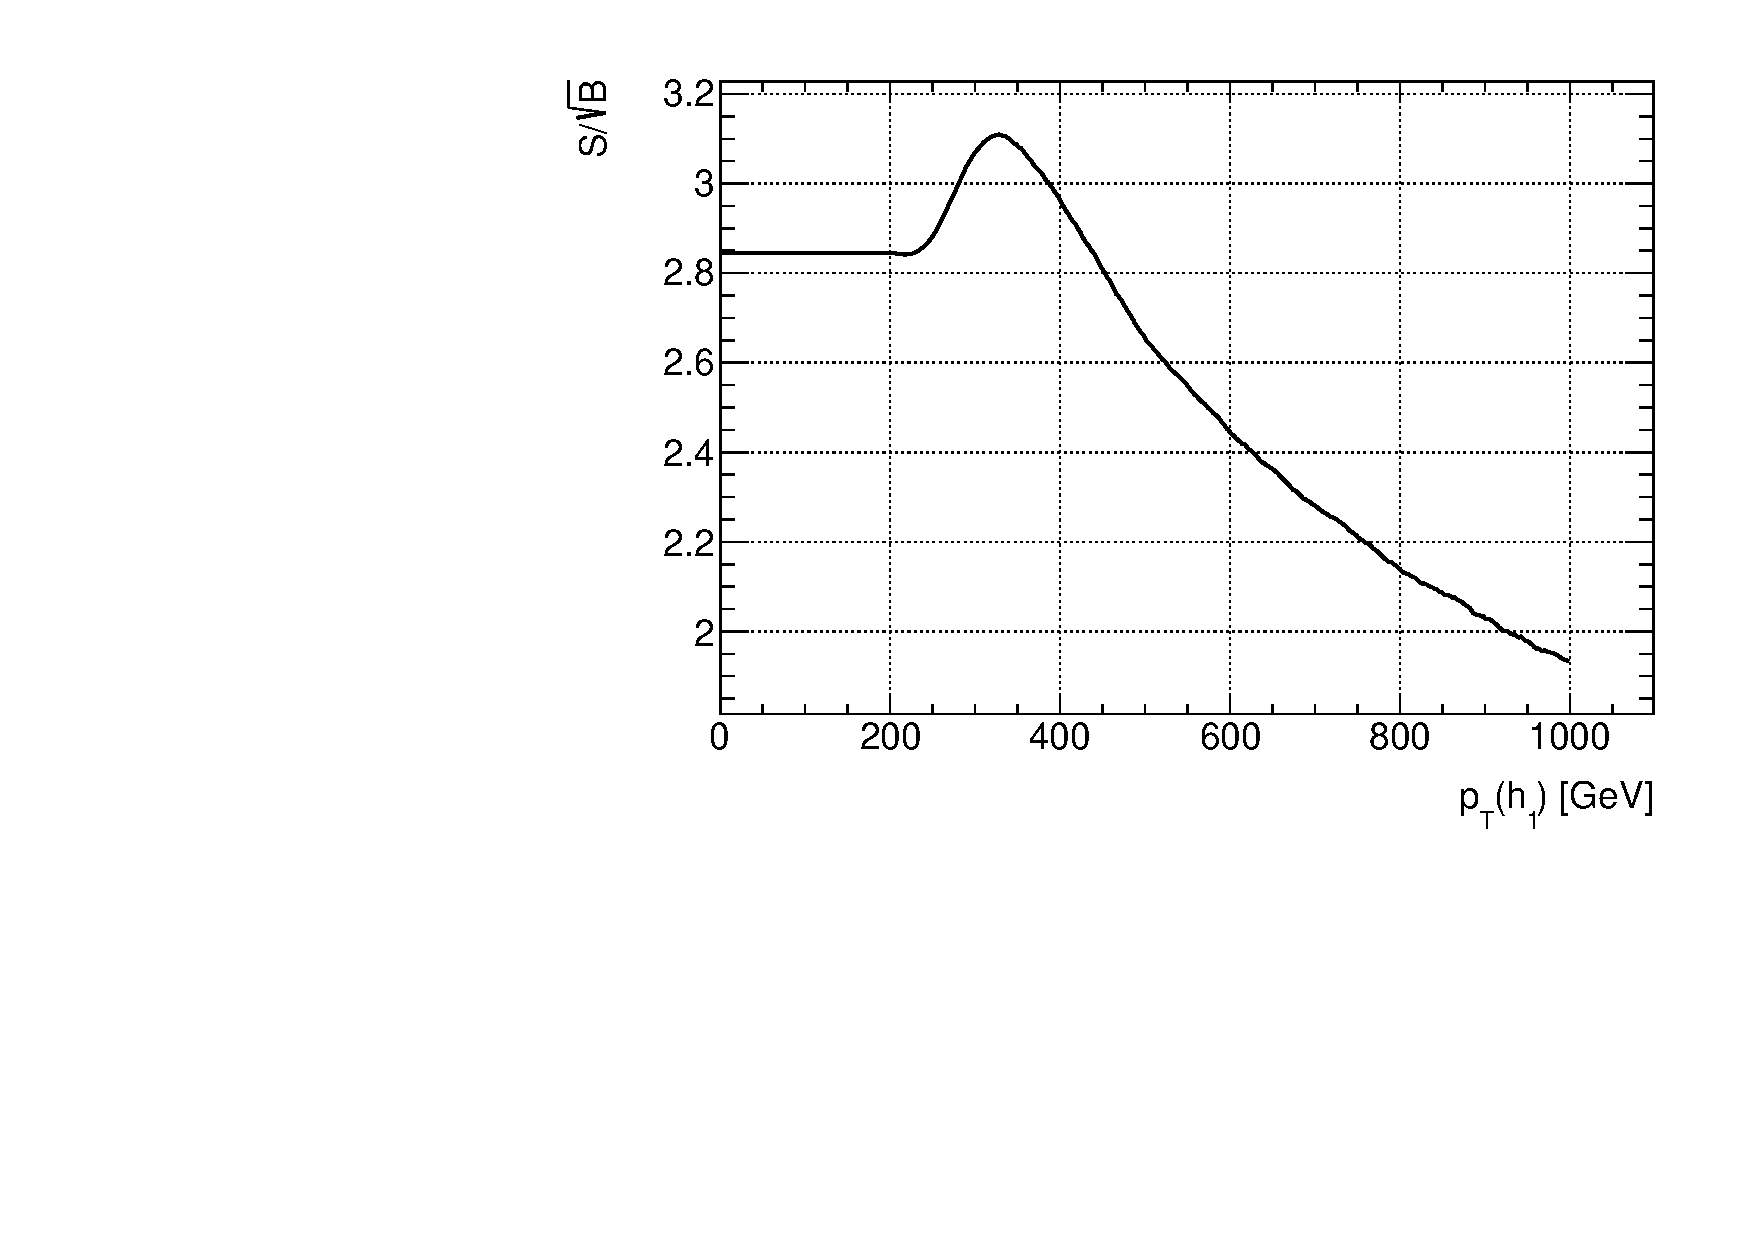
\includegraphics[trim={.6cm 0 0 0},clip,width=\linewidth]{./Figures/SSB_h1_pt.pdf}
		%\caption{oi}
		%\label{fig:h1_pt}
	\end{minipage}%
	\begin{minipage}{.5\textwidth}
		\centering
		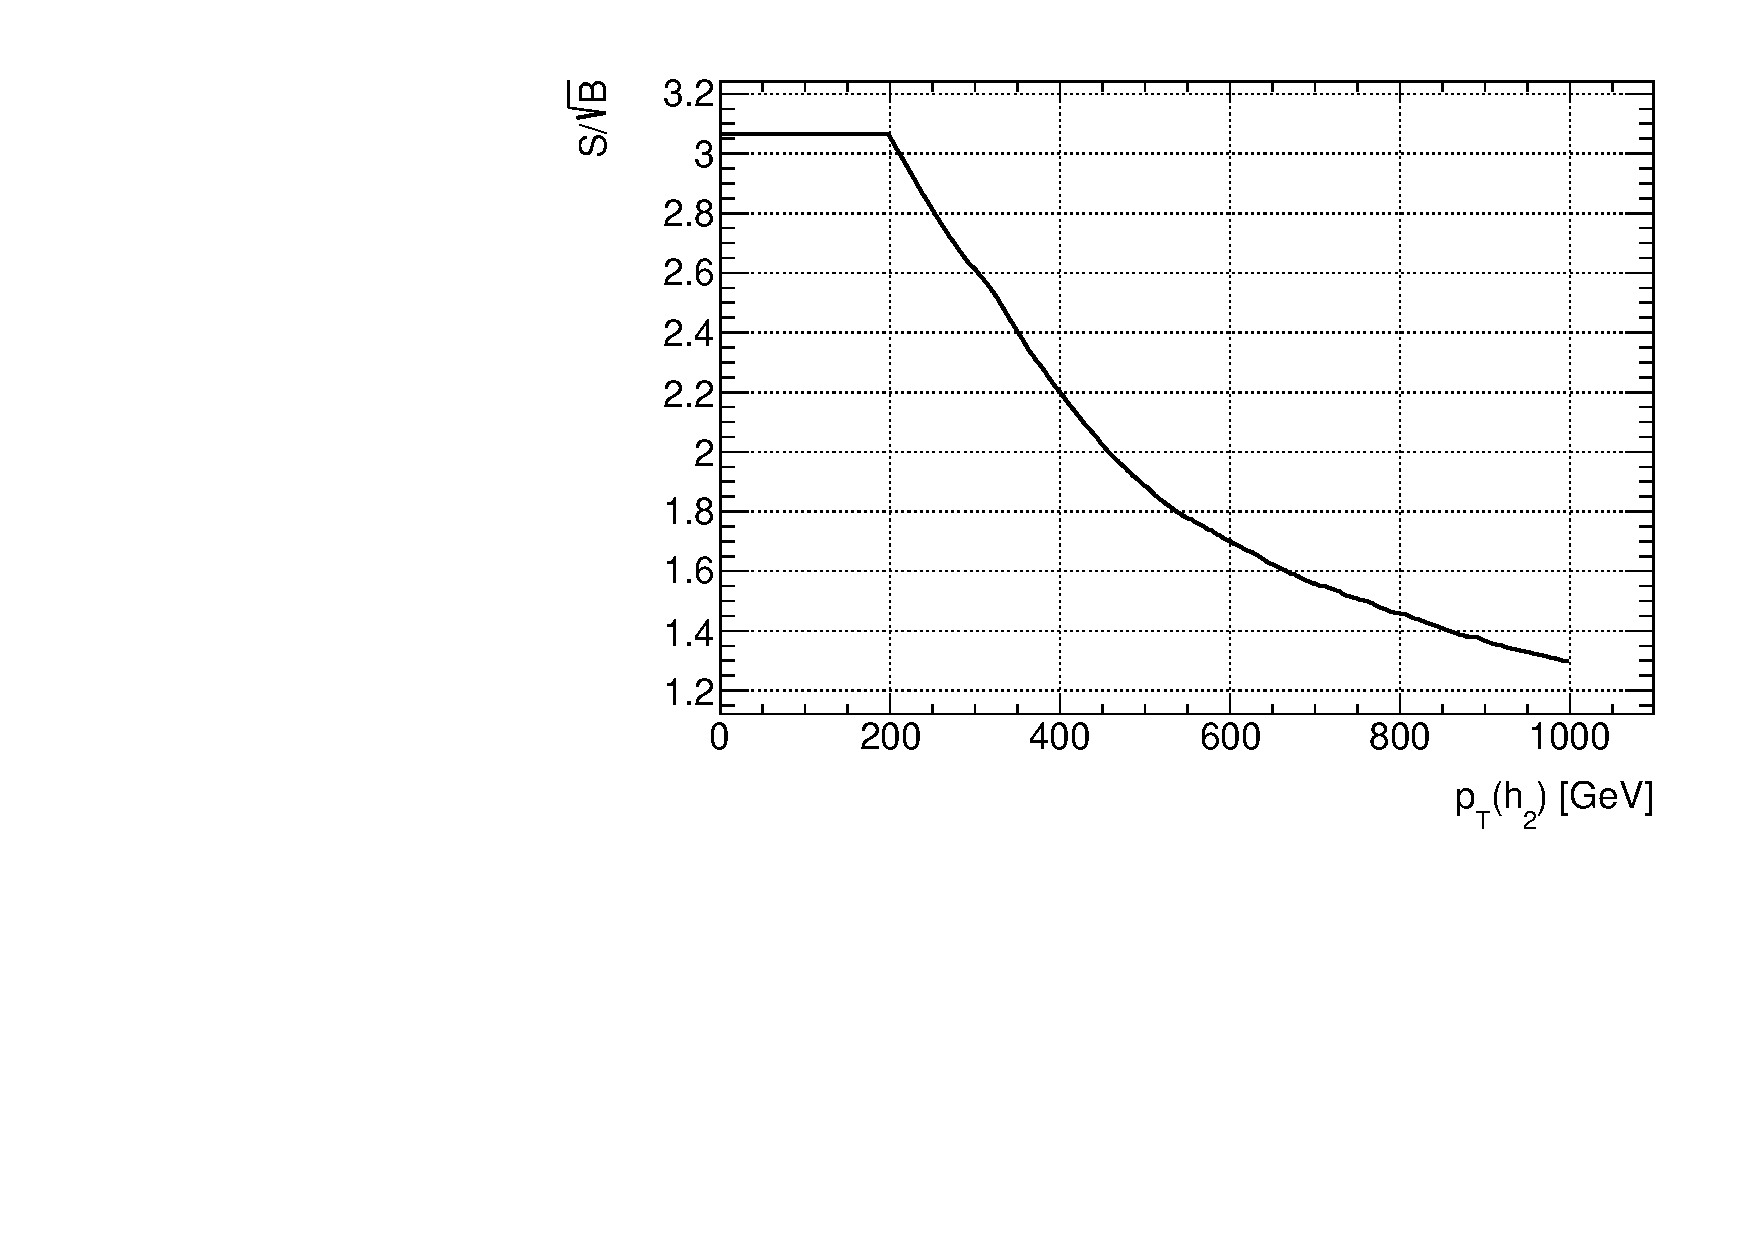
\includegraphics[trim={0 0 .6cm 0},clip,width=\linewidth]{./Figures/SSB_h2_pt.pdf}
		%\caption{oi}
		%\label{fig:h2_pt}
	\end{minipage}
	\begin{minipage}[t]{0.5\textwidth}
		\caption*{(a)}
		%\label{fig1}
	\end{minipage}%%%
	\hfill
	\begin{minipage}[t]{0.5\textwidth}
		\caption*{(b)}
		%\label{fig2}
	\end{minipage}
	\caption{$S/\sqrt{B}$ as a function of the cut on the $p_T$ of the leading Higgs candidate, $p_T(h_1)$ (a) after the pre-selection cuts and of the sub leading Higgs candidate, $p_T(h_2)$ (b) after the cut on $p_T(h_1)$.}
	\label{fig:SSB_h1h2_pt}
\end{figure} 

\begin{figure}
	\centering
	\begin{minipage}{.5\textwidth}
		\centering
		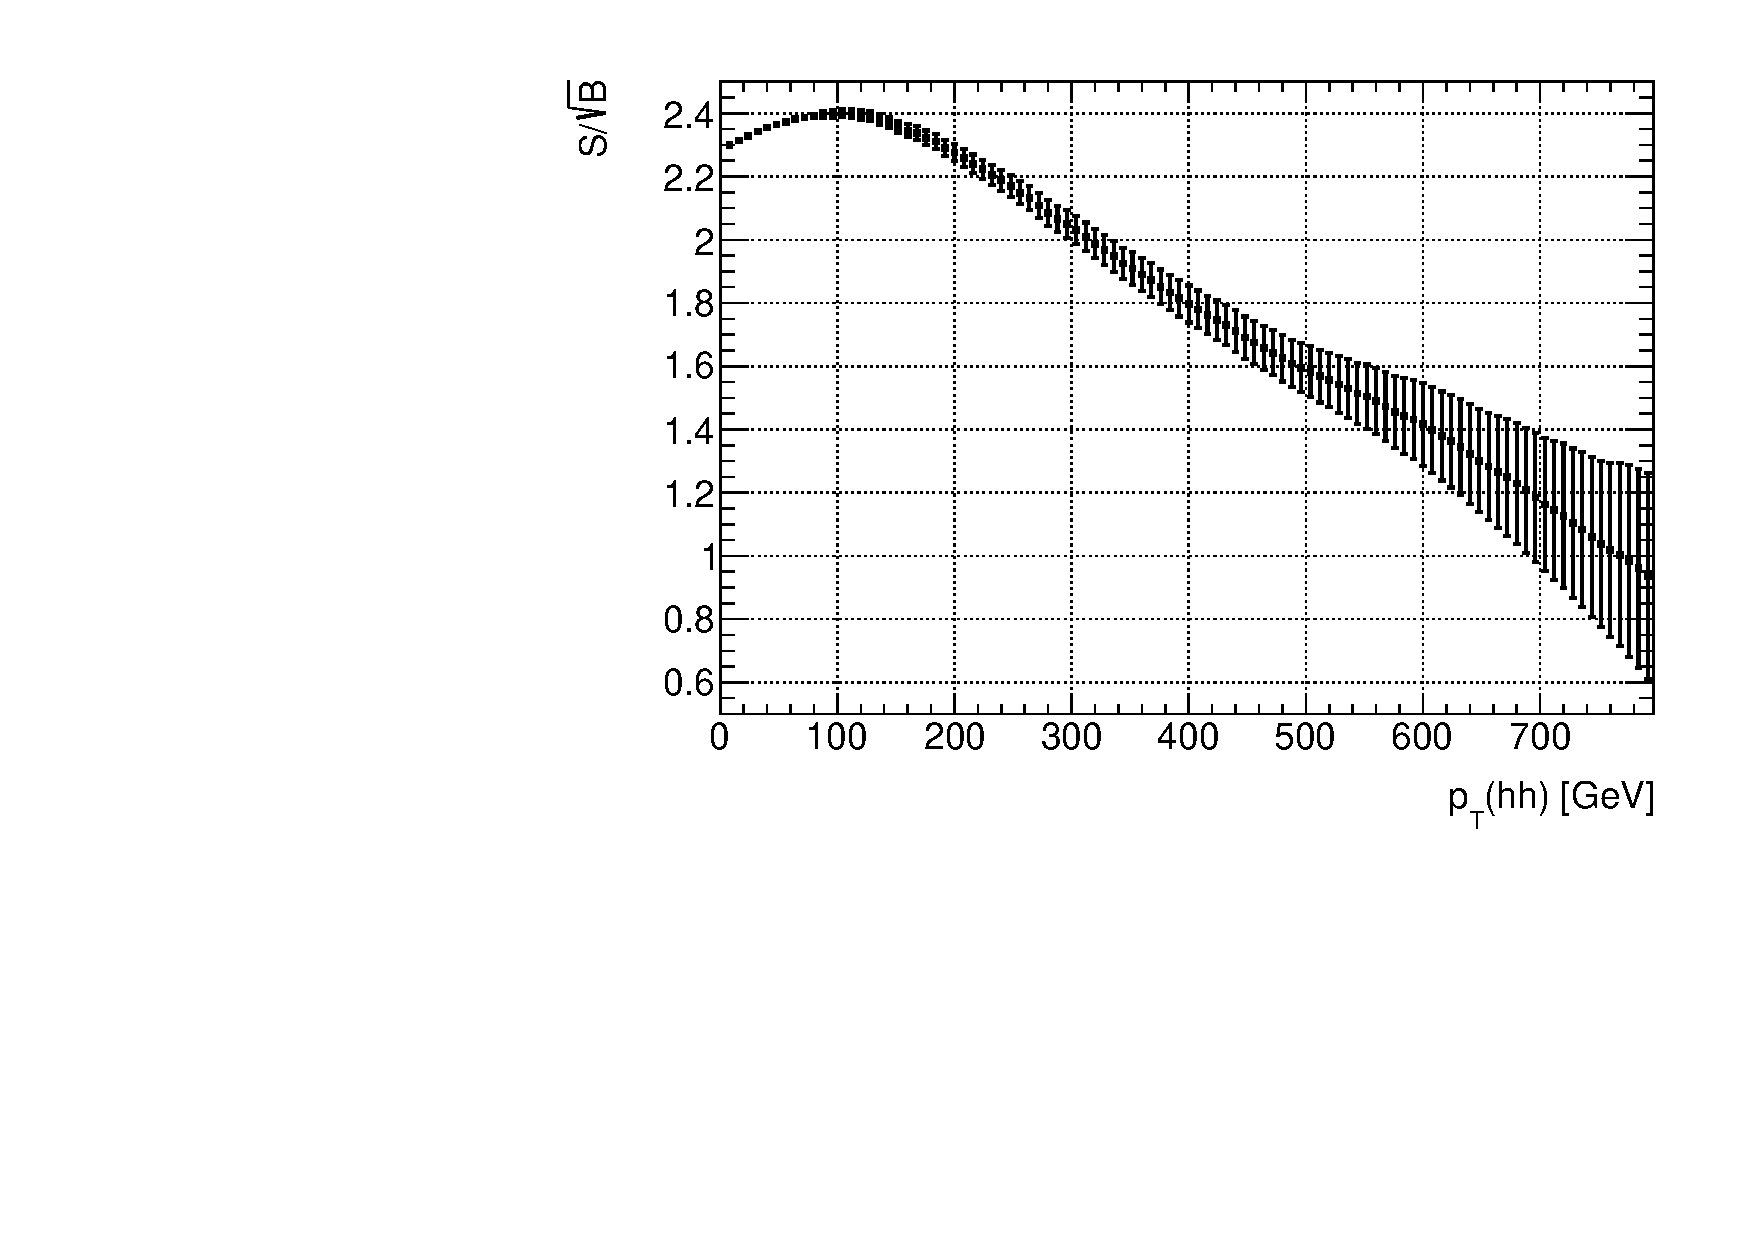
\includegraphics[trim={.6cm 0 0 0},clip,width=\linewidth]{./Figures/SSB_hh_pt.pdf}
		%\caption{oi}
		%\label{fig:h1_pt}
	\end{minipage}%
	\begin{minipage}{.5\textwidth}
		\centering
		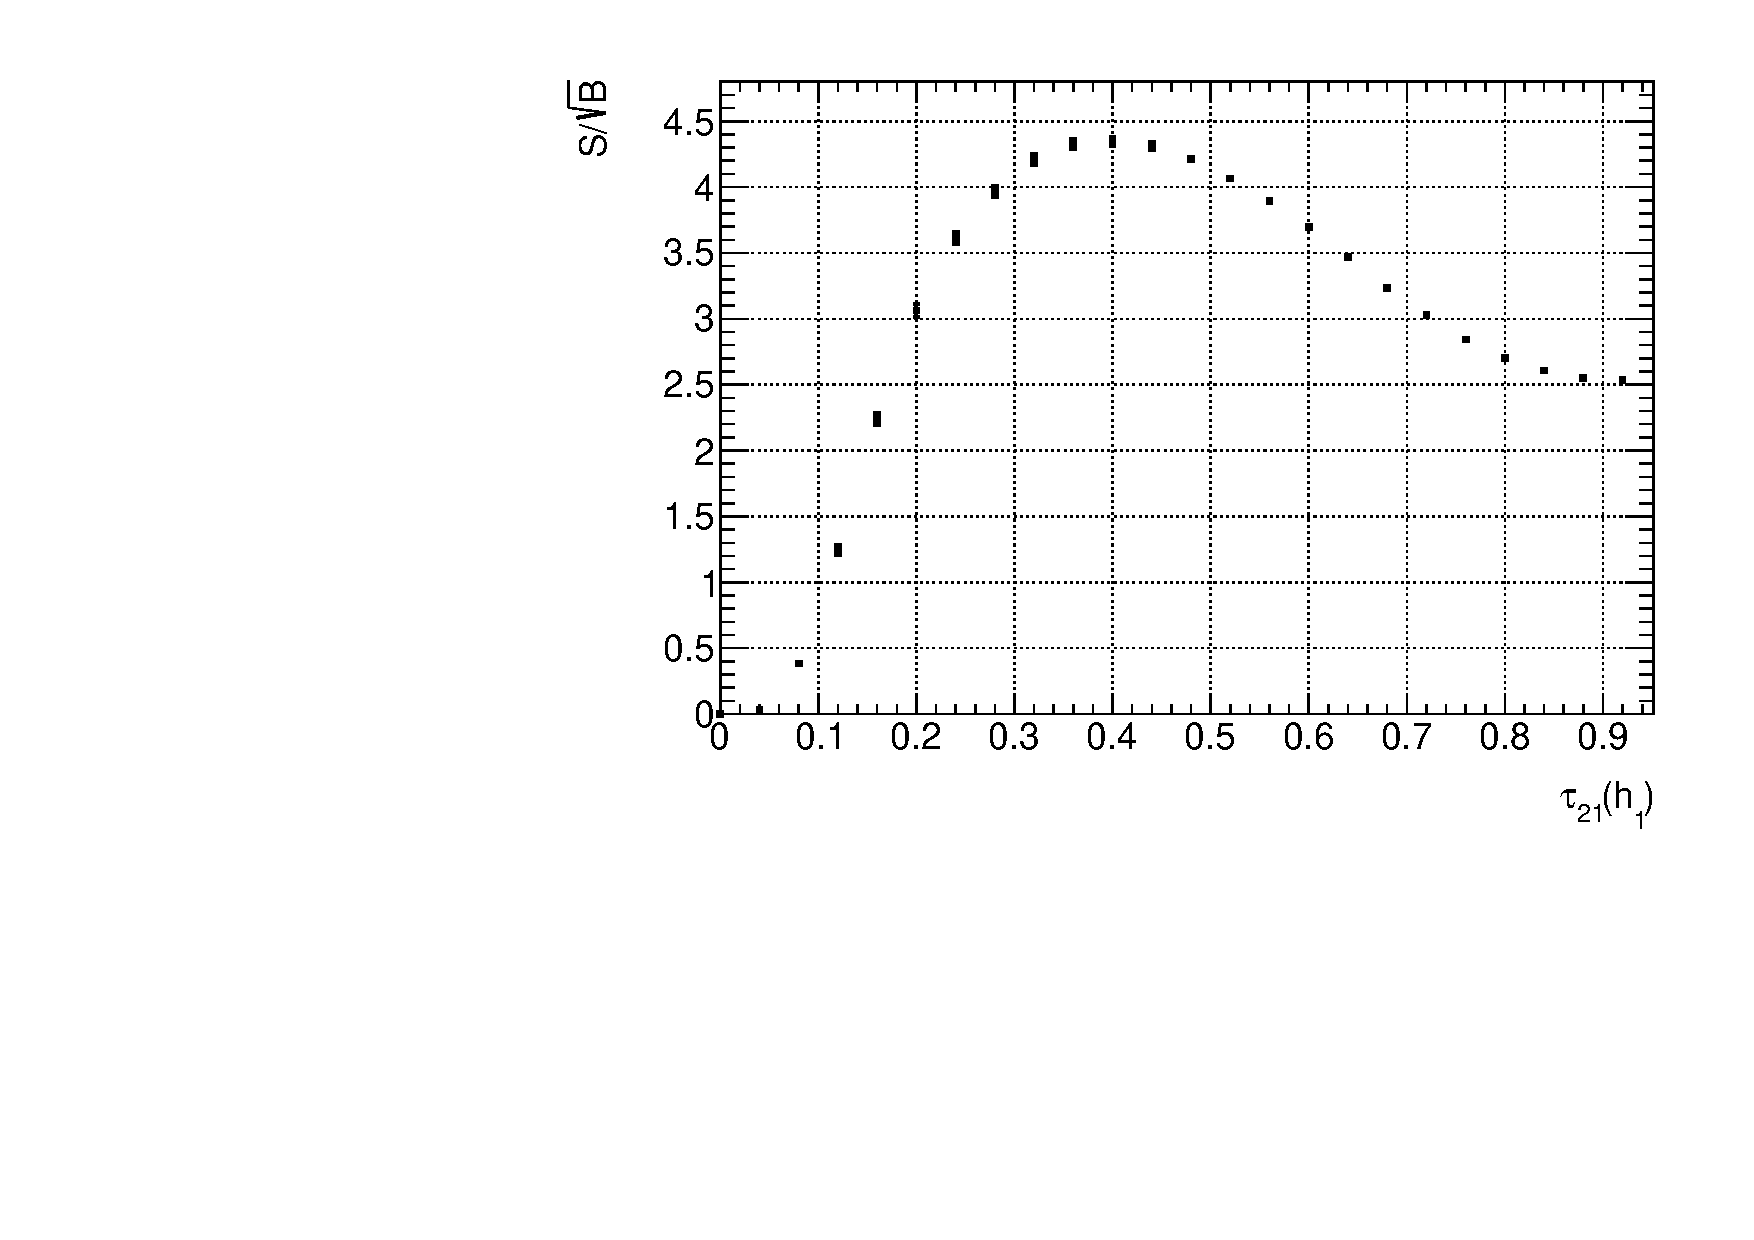
\includegraphics[trim={0 0 .65cm 0},clip,width=\linewidth]{./Figures/SSB_h1_tau21.pdf}
		%\caption{oi}
		%\label{fig:h2_pt}
	\end{minipage}
	\begin{minipage}[t]{0.5\textwidth}
		\caption*{(a)}
		%\label{fig1}
	\end{minipage}%%%
	\hfill
	\begin{minipage}[t]{0.5\textwidth}
		\caption*{(b)}
		%\label{fig2}
	\end{minipage}
	\caption{$S/\sqrt{B}$ as a function of the cut on the $p_T$ of the Higgs pair, $p_T(hh)$ (a) after the cut on $p_T(h_1)$ and as a function of the $\tau_{21}$ variable for leading Higgs candidate, $\tau_{21}(h_1)$ (b) after the cut on $p_T(hh)$.}
	\label{fig:SSB_hh_pt}
\end{figure} 

\begin{figure}
	\centering
	\begin{minipage}{.5\textwidth}
		\centering
		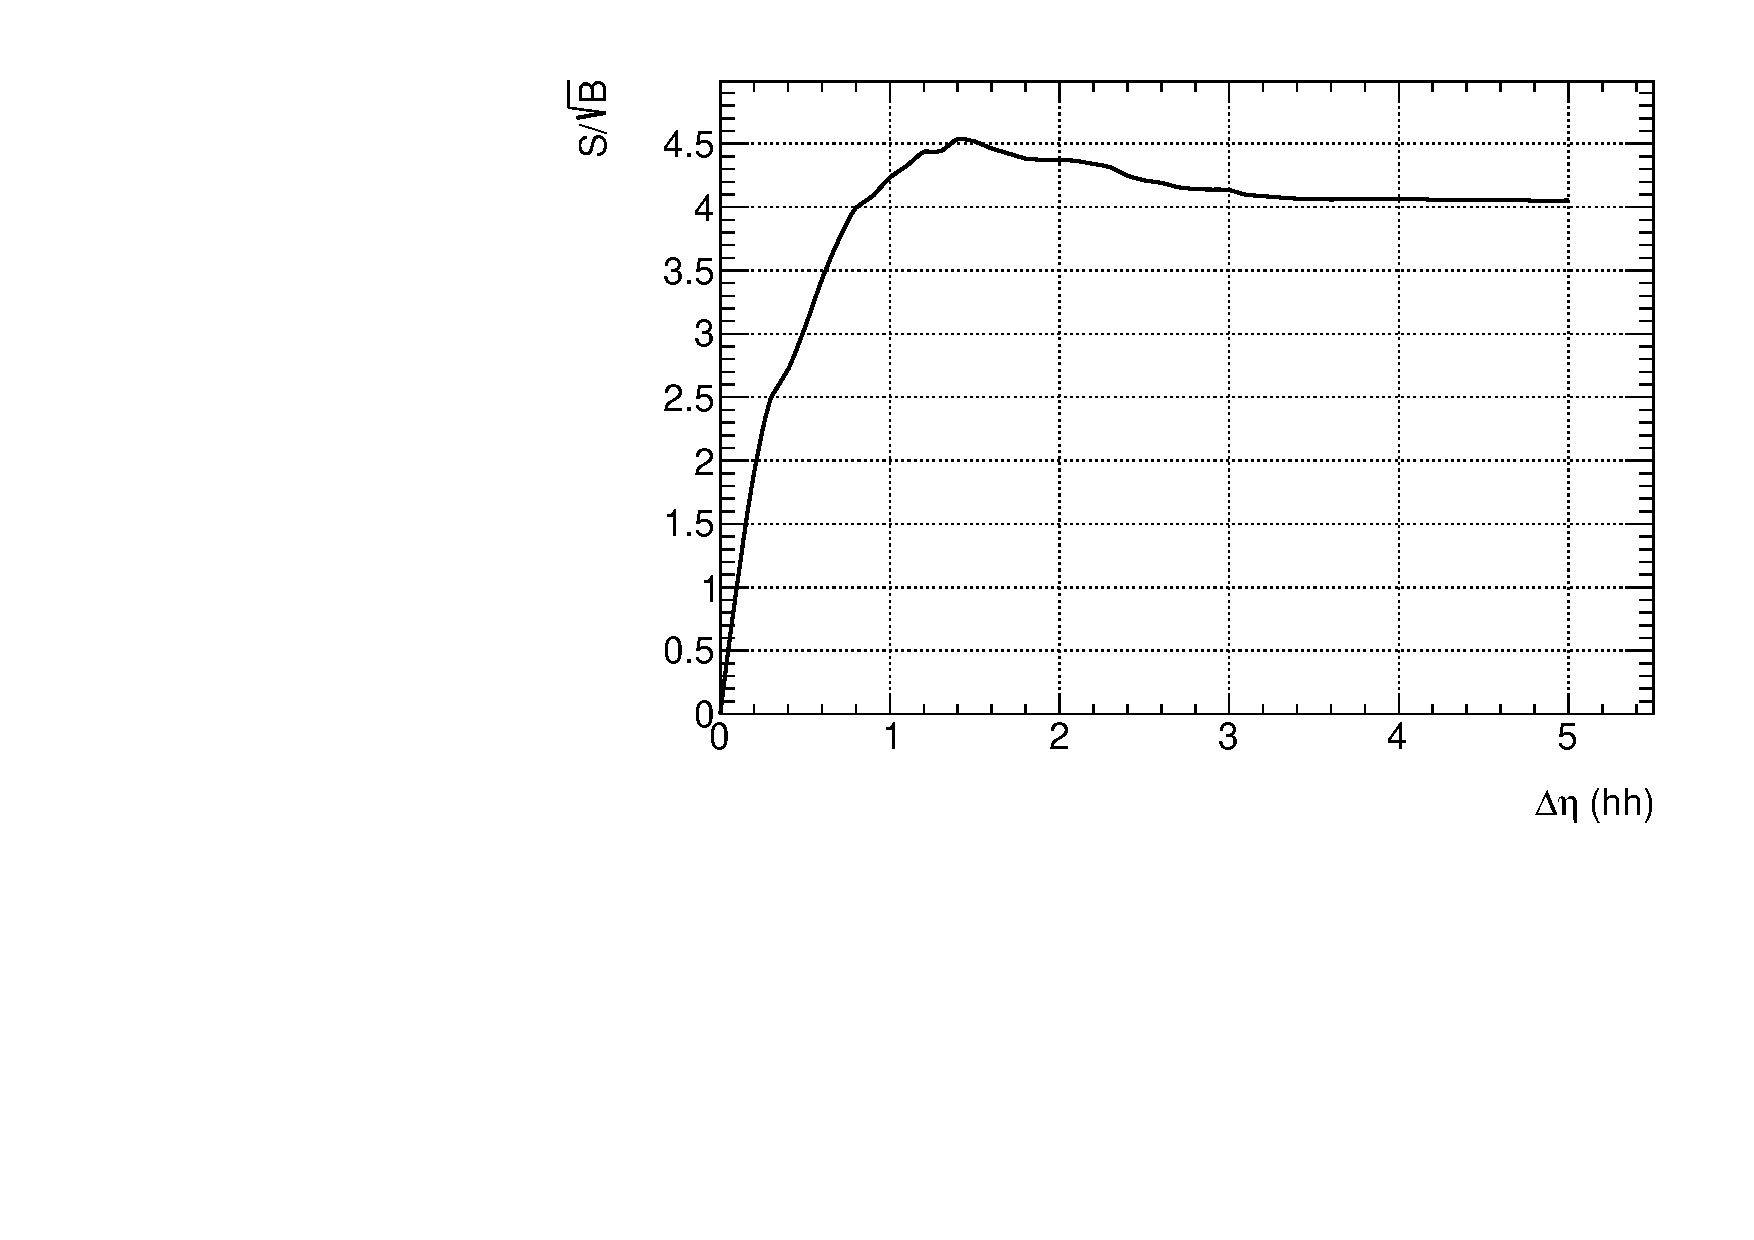
\includegraphics[trim={.6cm 0 0 0},clip,width=\linewidth]{./Figures/SSB_hh_deltaEta.pdf}
		%\caption{oi}
		%\label{fig:h1_pt}
	\end{minipage}%
	\begin{minipage}{.5\textwidth}
		\centering
		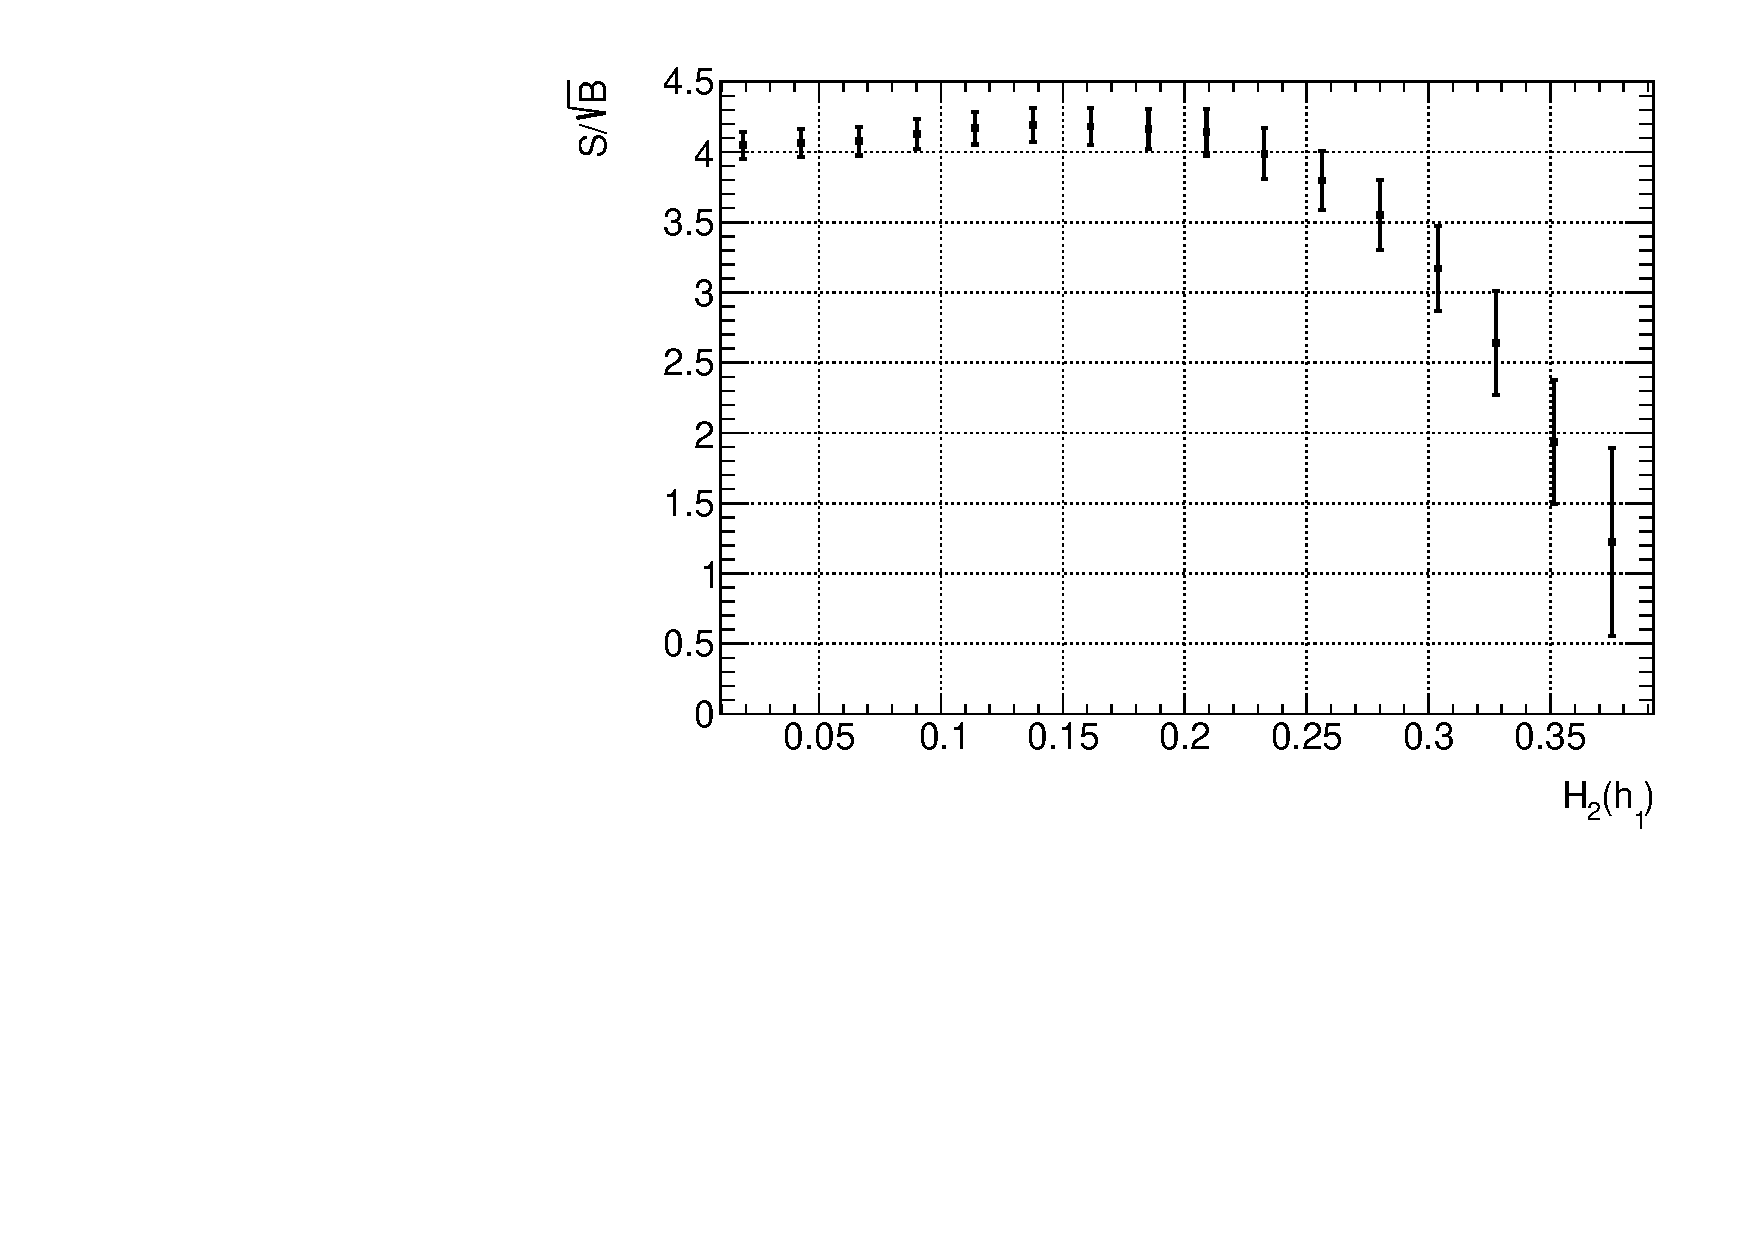
\includegraphics[trim={0 0 .6cm 0},clip,width=\linewidth]{./Figures/SSB_h1_FW2.pdf}
		%\caption{oi}
		%\label{fig:h2_pt}
	\end{minipage}
	\begin{minipage}[t]{0.5\textwidth}
		\caption*{(a)}
		%\label{fig1}
	\end{minipage}%%%
	\hfill
	\begin{minipage}[t]{0.5\textwidth}
		\caption*{(b)}
		%\label{fig2}
	\end{minipage}
	\caption{$S/\sqrt{B}$ as a function of the cut on the $\Delta\eta$ between the Higgs candidates, $\Delta\eta(hh)$ (a) after the cuts on the transverse momenta and on the $\tau_{21}$ variables and as a function of the second Fox-Wolfram momentum for the leading Higgs candidate, $H_l(h_1)$ (b) after the cuts on the transverse momentums, $\tau_{21}$ and $\Delta\eta$.}
	\label{fig:SSB_hh_deltaEta}
\end{figure} 

\subsection{Handling of uncertainties}

\subsubsection{Statistical uncertainties}

%In this work, only statistical uncertainties are considered. This is due to the exploratory nature of this analysis but also because systematic uncertainties are usually related to the detector and object reconstruction specificities making them difficult to list and quantify for a detector that is not yet built.

For challenging analyses such as this one, the backgrounds usually have a much larger cross section than the signal, implying that we need large of Monte Carlo samples to properly simulate them. Most of the times it is not feasible to generate as much events as one would need for a given luminosity. This is the case with this work, in particular because we are targeting very high luminosities (of the order of tens of $\text{ab}^{-1}$). Take for example the multijet sample with $500<H_T<1000$, where $H_T$ is the scalar sum of the $p_T$ of all partons at generator level. The cross section is approximately $10^7$ pb which means that we expect a total of $3\times 10^{14}$ events for an integrated luminosity of $30~\text{ab}^{-1}$. It is not feasible, within the time frame of this work and with the available computational resources, to generate this number of events. Therefore, we apply a weight, $w$, to each event given by:	
\begin{equation}
	w=\frac{\mathcal{L}\times \sigma}{N}
\end{equation}
where $\mathcal{L}$ is the target integrated luminosity, $\sigma$ is the cross section of the sample and $N$ is the number of MC events generated.

If we assume that the number of events follows a Poisson distribution then the standard deviation (or uncertainty) is given by $\sqrt{N}$ where $N$ is the mean number of events. In order to normalize the number of events to a given luminosity we need to multiply the mean value and the uncertainty by the respective weight such that the number of normalized events, including the uncertainty, $N_{\text{norm}}\pm \Delta N_{\text{norm}}$, is given by:
\begin{equation}
	N_{\text{norm}}\pm \Delta N_{\text{norm}}=w\times \left(N \pm \sqrt{N}\right).
\end{equation}
$\Delta N_{\text{norm}}$ can then be used in standard error propagation to compute the statistical uncertainty associated with any expression, in particular, with $S/\sqrt{B}$. The statistical error associated with $S/\sqrt{B}$ is given by:
\begin{equation}
	\left(\Delta\frac{S}{\sqrt{B}}\right)_{\text{stat.}}^2=\left|\frac{1}{\sqrt{B}}\right|^2 (\Delta S)^2+\left|-\frac{S}{B^{3/2}}\right|^2 (\Delta B)^2
	\label{eq:stat}
\end{equation}
where $\Delta S$ and $\Delta B$ are the uncertainties associated with the number of signal and background events. $\Delta B$ is given by:
\begin{equation}
		(\Delta B)^2 =\sum_i (\Delta B_i)^2
\end{equation}
where the index $i$ runs over all independent backgrounds.

\subsubsection{Systematic uncertainties}
\label{sec:sys_unc}

Systematic uncertainties are usually related to the detector specificities and object reconstruction techniques, which makes them difficult to list and quantify for a detector that is not yet built. Nonetheless, we can use the numbers for the systematic uncertainties that are reported in existing searches for $pp\rightarrow hh\rightarrow b\overline{b}b\overline{b}$ using the ATLAS detector.

When requiring four b-tags, the largest uncertainty affecting the signal is the the b-tagging uncertainty (table 6 of Ref. \cite{hh2bbbbATLAS1}). It is of the order of $30\%$.
For the background, the largest uncertainty comes from the estimation of its yield and shape, according to the same reference. The reported value is $16\%$. However, a study performed by the FCC study group \cite{FCCphysClement} considers more conservative values for the uncertainties on the $t\overline{t}$ and  QCD di-jet backgrounds normalizations. The reported values are $20\%$ for $t\overline{t}$ and $50\%$ for di-jet production. In this study we use these numbers to estimate the impact of the systematic uncertainties on the normalization of the backgrounds, sice they give a more conservative estimate.

To estimate the b-tagging systematic uncertainty, the number of signal events after all the analysis cuts is varied by $30\%$ up and down. This leads to an upper (lower) bound in the significance of $6.6~(3.6)$, considering the baseline analysis. This uncertainty is applied to signal only. According to Ref. \cite{hh2bbbbATLAS1}, the b-tagging systematic uncertainty for the background is a lot smaller than for the signal ($\sim 1\%$ compared to $\sim30\%$). Nonetheless, it could become relevant for the $4b+j$ background. However, for the multijet background, the dominant systematic uncertainty is on its normalization. We consider a value of $50\%$ which clearly dominates over the b-tagging systematic uncertainty even if we consider that it takes a value of $30\%$ for the $4b+j$ background.

The background normalization uncertainties are implemented by increasing and decreasing the k-factor of each background by the corresponding percentage, with respect to what is given in table \ref{table:samples_summary}. We vary the k-factors of the QCD multijet ($4b+j$ and $jj+0/1/2 ~j$) and of the $t\overline{t}$ backgrounds individually. For the $4b+j$ and $jj+0/1/2 ~j$ backgrounds we consider the same uncertainty of $50\%$ and the variations are done simultaneously for both. This leads to an upper (lower) bound in the significance of $7.1~(4.2)$. For the $t\overline{t}$ background we consider an uncertainty of $20\%$ which leads to an upper (lower) bound in the significance of $5.13~(5.09)$. These numbers refer to the baseline analysis.

We assume that the three sources of systematic uncertainty are uncorrelated and therefore the respective variations can be added in quadrature. The statistical error is also added in quadrature. Therefore, the total uncertainty is given by:
\begin{equation}
	\left(\Delta\frac{S}{\sqrt{B}}\right)_{\text{sys.+stat.}}^2=\left(\delta_{\text{b-tag}}\right)^2+\left(\delta_{\text{QCD bkg.}}\right)^2+\left(\delta_{t\overline{t}~\text{bkg.}}\right)^2+\left(\delta_{\text{stat.}}\right)^2
\end{equation}
where $\delta_{\text{b-tag}},\delta_{\text{QCD bkg.}}$ and $\delta_{t\overline{t}~\text{bkg.}}$ are the variations with respect to the nominal value of the significance caused by the b-tagging uncertainty and by the uncertainties on the normalization of the  QCD multijet and $t\overline{t}$ backgrounds, respectively. $\delta_{\text{stat.}}$ is the statistical uncertainty, given by Eq. \ref{eq:stat}. 

\subsection{Trigger discussion}

In the previous discussions regarding the baseline and optimized analysis, no trigger requirements were taken into account. We now review the trigger requirements that had to be fulfilled in the analysis performed by ATLAS and discuss where do the analyses we designed stand with respect to those requirements. 

In Ref. \cite{hh2bbbbATLAS1}, the event selection requires the existence of at least two anti-$k_T$ $R=1.0$ jets with $p_T>250$ GeV, $|\eta|<2.0$ and $m_J>50$ GeV. In addition, the leading jet must have $p_T>450$ GeV to guarantee $100\%$ trigger efficiency. 

We require at least two anti-$k_T$ $R=0.8$ jets with $p_T>200$ GeV. In the baseline analysis, we require that the leading jet has $p_T>400$ GeV. These $p_T$ thresholds are compatible to the ones used in the ATLAS analysis mainly when we consider that the radius of the jets is slightly smaller and therefore the $p_T$ threshold can also be lower. We do not consider any cuts on the pseudorapidity or mass of the jets. However, we do require that the sub leading jet has $p_T>300$ GeV and that the Higgs pair has $p_T>100$ GeV which would help lower the rate. 

In the optimized analysis, however, the $p_T$ cuts are significantly looser: the leading jet must have $p_T>300$ GeV and the Higgs pair must have $p_T>100$ GeV. This could indicate that although the optimized analysis gives a better significance, tighter cuts might have to be applied in order to fulfill the trigger requirements, therefore reducing the significance.

%% ----------------------------------------------------------------------
%\subsection{Intermediate}20
%\label{section:intermediate}
%
%- Event topology: one large R jet corresponding to the leading Higgs candidate and two small R jets corresponding to the b quarks of the sub leading Higgs candidate \\
%- Physics objects: fat jets (already described in previous section) and particle flow anti-kT R=0.4 jets \\
%- Selection criteria \\
%- Substructure variables: refer we (can)apply them to the fat jet \\
%- Optimization\\
%-------------------------------------------------------------------
% 
%This category targets events in which one of the Higgs bosons has a high Lorentz boost and therefore is reconstructed using a particle flow, anti-$k_T$ jet with $R=0.8$ (large-R jets). This is assumed to be the leading Higgs candidate. The sub leading Higgs boson, due to its relatively low $p_T$, can be fully reconstructed, meaning that each b quark is reconstructed using particle flow, anti-$k_T$ jets with $R=0.4$ (small-R jets). For the large-R jets the b-tagging is performed as described in the previous section. The small-R jets are b-tagged using Delphes default algorithm.
%
%\subsubsection{Event selection}
%
%We require exactly one large-R jet and at least two small-R jets. All jets have to be within $|\eta|<6$. The large-R jet is required to have $p_T>200$ GeV and the small-R jets are required to have $p_T>50$ GeV.
%% ----------------------------------------------------------------------
%\subsection{Resolved}
%\label{section:resolved}
%
%- Event topology: 4 small-R jets \\
%- Physics objects: small R jets already described in previous section \\
%- Selection criteria \\
%- Optimization (angular variables between b quarks, ...)\\
%-------------------------------------------------------------------
%
%This analysis category targets events in which the four b quarks can be reconstructed in four individual jets.
%
%The events are reconstructed using particle flow jets with $R=0.4$, clustered with the anti-$k_T$ algorithm. The b tagging is done using Delphes default algorithm.